 \documentclass[oneside,a4paper,12pt]{book}
%\pagestyle{headings}
\frontmatter

% !TEX encoding = UTF-8 Unicode

%=============================================================================

% Just add % !TEX encoding = UTF-8 Unicode

%=============================================================================

% Just add % !TEX encoding = UTF-8 Unicode

%=============================================================================

% Just add \input{smalltalkEnv} to your file
% then you can use :
% \begin{lstlisting}[language=Smalltalk]
% false become: true.
% \end{lstlisting}


\usepackage{color}
\usepackage{listings}
\usepackage{etoolbox}
\usepackage{textcomp}
\usepackage{xpatch}
\usepackage{tcolorbox}

\definecolor{source}{gray}{0.95}

\definecolor{stComment}{rgb}{0.5,0.5,0.5}
\definecolor{stString}{rgb}{0.58,0,0.82}
\definecolor{stKeywords}{rgb}{0.21,0.55,0.7}
\definecolor{stNumbers}{rgb}{.5,0,0}

\newtoggle{InString}{}% Keep track of if we are within a string
\togglefalse{InString}% Assume not initally in string
\newcommand*{\ColorIfNotInString}[1]{\iftoggle{InString}{#1}{\color{stNumbers}#1}}%
\newcommand*{\ProcessQuote}[1]{#1\iftoggle{InString}{\global\togglefalse{InString}}{\global\toggletrue{InString}}}%

\lstdefinelanguage{Smalltalk}{
  basicstyle=\sffamily\scriptsize,
  keywordstyle=\color{stKeywords},
  commentstyle=\color{stComment},
  stringstyle=\color{stString},
  alsoletter=\#,
  identifierstyle=\idstyle, 
  showstringspaces=false,
  morekeywords={true,false,self,super,nil},
  backgroundcolor=\color{source},
  sensitive=true, 
  morecomment=[s]{"}{"}, 
  morestring=[d]', 
  style=SmalltalkStyle,
  literate=
    {BANG}{!}1
    {UNDERSCORE}{\_}1
    {\\st}{Smalltalk}9 % convenience -- in case \st occurs in code
    % {'}{{\textquotesingle}}1 % replaced by upquote=true in \lstset
    {_}{{$\leftarrow$}}1
    {>>>}{{\sep}}1
    {^}{{$\uparrow$}}1
    {~}{{$\sim$}}1
    {-}{{\sf -\hspace{-0.13em}-}}1  % the goal is to make - the same width as +
    {+}{\raisebox{0.08ex}{+}}1		% and to raise + off the baseline to match -
    {-->}{{\quad$\longrightarrow$\quad}}3
	, % Don't forget the comma at the end!
  tabsize=2,
}



\makeatletter%
\newcommand*\idstyle[1]{%
  \expandafter\id@style\the\lst@token{#1}\relax%
}
\def\id@style#1#2\relax{%
  \ifnum\pdfstrcmp{#1}{\#}=0%
  \color{stString} \the\lst@token%
  \else%
  \edef\tempa{\uccode`#1}%
  \edef\tempb{`#1}%
  \ifnum\tempa=\tempb%
  \color{blue} \the\lst@token%
  \else%
  \the\lst@token%
  \fi%
  \fi%
}

\lstdefinestyle{SmalltalkStyle}{ 
  literate=%
  {^}{{$\uparrow$}}1% 
  % {"}{{{\ProcessQuote{"}}}}1% Disable coloring within double quotes
  % {'}{{{\ProcessQuote{'}}}}1% Disable coloring within single quote
  {0}{{{\ColorIfNotInString{0}}}}1%
  {1}{{{\ColorIfNotInString{1}}}}1%
  {2}{{{\ColorIfNotInString{2}}}}1%
  {3}{{{\ColorIfNotInString{3}}}}1%
  {4}{{{\ColorIfNotInString{4}}}}1%
  {5}{{{\ColorIfNotInString{5}}}}1%
  {6}{{{\ColorIfNotInString{6}}}}1%
  {7}{{{\ColorIfNotInString{7}}}}1%
  {8}{{{\ColorIfNotInString{8}}}}1%
  {9}{{{\ColorIfNotInString{9}}}}1%
} 

\lstset{% setup listings
    framexleftmargin=6pt,
    framextopmargin=6pt,
    framexbottommargin=6pt, 
    frame=tb, framerule=0pt,
}


% In-line code (literal)  with background color
% Normally use this for all in-line code:
\newcommand{\ct}[1]{{\colorbox{source}{\lstinline[mathescape=false,backgroundcolor=\color{source},basicstyle={\sffamily\small}]{#1}}}}


% In-line code (latex enabled)
% Use this only in special situations where \ct does not work
% (within section headings ...):
\newcommand{\lct}[1]{{\textsf{\textup{#1}}}}
% Code environments
\lstnewenvironment{code}{%
	\lstset{%
	    escapeinside={(*@}{@*)},
		% frame=lines,
		frame=single,
		framerule=0pt,
		mathescape=false
	}%
}{%
}


\newcommand*\DNumber{\addtocounter{lstnumber}{-1}}
%%% Always I forget this so I created some aliases
\def\ContinueLineNumber{\lstset{firstnumber=last}}
\def\StartLineAt#1{\lstset{firstnumber=#1}}
\let\numberLineAt\StartLineAt to your file
% then you can use :
% \begin{lstlisting}[language=Smalltalk]
% false become: true.
% \end{lstlisting}


\usepackage{color}
\usepackage{listings}
\usepackage{etoolbox}
\usepackage{textcomp}
\usepackage{xpatch}
\usepackage{tcolorbox}

\definecolor{source}{gray}{0.95}

\definecolor{stComment}{rgb}{0.5,0.5,0.5}
\definecolor{stString}{rgb}{0.58,0,0.82}
\definecolor{stKeywords}{rgb}{0.21,0.55,0.7}
\definecolor{stNumbers}{rgb}{.5,0,0}

\newtoggle{InString}{}% Keep track of if we are within a string
\togglefalse{InString}% Assume not initally in string
\newcommand*{\ColorIfNotInString}[1]{\iftoggle{InString}{#1}{\color{stNumbers}#1}}%
\newcommand*{\ProcessQuote}[1]{#1\iftoggle{InString}{\global\togglefalse{InString}}{\global\toggletrue{InString}}}%

\lstdefinelanguage{Smalltalk}{
  basicstyle=\sffamily\scriptsize,
  keywordstyle=\color{stKeywords},
  commentstyle=\color{stComment},
  stringstyle=\color{stString},
  alsoletter=\#,
  identifierstyle=\idstyle, 
  showstringspaces=false,
  morekeywords={true,false,self,super,nil},
  backgroundcolor=\color{source},
  sensitive=true, 
  morecomment=[s]{"}{"}, 
  morestring=[d]', 
  style=SmalltalkStyle,
  literate=
    {BANG}{!}1
    {UNDERSCORE}{\_}1
    {\\st}{Smalltalk}9 % convenience -- in case \st occurs in code
    % {'}{{\textquotesingle}}1 % replaced by upquote=true in \lstset
    {_}{{$\leftarrow$}}1
    {>>>}{{\sep}}1
    {^}{{$\uparrow$}}1
    {~}{{$\sim$}}1
    {-}{{\sf -\hspace{-0.13em}-}}1  % the goal is to make - the same width as +
    {+}{\raisebox{0.08ex}{+}}1		% and to raise + off the baseline to match -
    {-->}{{\quad$\longrightarrow$\quad}}3
	, % Don't forget the comma at the end!
  tabsize=2,
}



\makeatletter%
\newcommand*\idstyle[1]{%
  \expandafter\id@style\the\lst@token{#1}\relax%
}
\def\id@style#1#2\relax{%
  \ifnum\pdfstrcmp{#1}{\#}=0%
  \color{stString} \the\lst@token%
  \else%
  \edef\tempa{\uccode`#1}%
  \edef\tempb{`#1}%
  \ifnum\tempa=\tempb%
  \color{blue} \the\lst@token%
  \else%
  \the\lst@token%
  \fi%
  \fi%
}

\lstdefinestyle{SmalltalkStyle}{ 
  literate=%
  {^}{{$\uparrow$}}1% 
  % {"}{{{\ProcessQuote{"}}}}1% Disable coloring within double quotes
  % {'}{{{\ProcessQuote{'}}}}1% Disable coloring within single quote
  {0}{{{\ColorIfNotInString{0}}}}1%
  {1}{{{\ColorIfNotInString{1}}}}1%
  {2}{{{\ColorIfNotInString{2}}}}1%
  {3}{{{\ColorIfNotInString{3}}}}1%
  {4}{{{\ColorIfNotInString{4}}}}1%
  {5}{{{\ColorIfNotInString{5}}}}1%
  {6}{{{\ColorIfNotInString{6}}}}1%
  {7}{{{\ColorIfNotInString{7}}}}1%
  {8}{{{\ColorIfNotInString{8}}}}1%
  {9}{{{\ColorIfNotInString{9}}}}1%
} 

\lstset{% setup listings
    framexleftmargin=6pt,
    framextopmargin=6pt,
    framexbottommargin=6pt, 
    frame=tb, framerule=0pt,
}


% In-line code (literal)  with background color
% Normally use this for all in-line code:
\newcommand{\ct}[1]{{\colorbox{source}{\lstinline[mathescape=false,backgroundcolor=\color{source},basicstyle={\sffamily\small}]{#1}}}}


% In-line code (latex enabled)
% Use this only in special situations where \ct does not work
% (within section headings ...):
\newcommand{\lct}[1]{{\textsf{\textup{#1}}}}
% Code environments
\lstnewenvironment{code}{%
	\lstset{%
	    escapeinside={(*@}{@*)},
		% frame=lines,
		frame=single,
		framerule=0pt,
		mathescape=false
	}%
}{%
}


\newcommand*\DNumber{\addtocounter{lstnumber}{-1}}
%%% Always I forget this so I created some aliases
\def\ContinueLineNumber{\lstset{firstnumber=last}}
\def\StartLineAt#1{\lstset{firstnumber=#1}}
\let\numberLineAt\StartLineAt to your file
% then you can use :
% \begin{lstlisting}[language=Smalltalk]
% false become: true.
% \end{lstlisting}


\usepackage{color}
\usepackage{listings}
\usepackage{etoolbox}
\usepackage{textcomp}
\usepackage{xpatch}
\usepackage{tcolorbox}

\definecolor{source}{gray}{0.95}

\definecolor{stComment}{rgb}{0.5,0.5,0.5}
\definecolor{stString}{rgb}{0.58,0,0.82}
\definecolor{stKeywords}{rgb}{0.21,0.55,0.7}
\definecolor{stNumbers}{rgb}{.5,0,0}

\newtoggle{InString}{}% Keep track of if we are within a string
\togglefalse{InString}% Assume not initally in string
\newcommand*{\ColorIfNotInString}[1]{\iftoggle{InString}{#1}{\color{stNumbers}#1}}%
\newcommand*{\ProcessQuote}[1]{#1\iftoggle{InString}{\global\togglefalse{InString}}{\global\toggletrue{InString}}}%

\lstdefinelanguage{Smalltalk}{
  basicstyle=\sffamily\scriptsize,
  keywordstyle=\color{stKeywords},
  commentstyle=\color{stComment},
  stringstyle=\color{stString},
  alsoletter=\#,
  identifierstyle=\idstyle, 
  showstringspaces=false,
  morekeywords={true,false,self,super,nil},
  backgroundcolor=\color{source},
  sensitive=true, 
  morecomment=[s]{"}{"}, 
  morestring=[d]', 
  style=SmalltalkStyle,
  literate=
    {BANG}{!}1
    {UNDERSCORE}{\_}1
    {\\st}{Smalltalk}9 % convenience -- in case \st occurs in code
    % {'}{{\textquotesingle}}1 % replaced by upquote=true in \lstset
    {_}{{$\leftarrow$}}1
    {>>>}{{\sep}}1
    {^}{{$\uparrow$}}1
    {~}{{$\sim$}}1
    {-}{{\sf -\hspace{-0.13em}-}}1  % the goal is to make - the same width as +
    {+}{\raisebox{0.08ex}{+}}1		% and to raise + off the baseline to match -
    {-->}{{\quad$\longrightarrow$\quad}}3
	, % Don't forget the comma at the end!
  tabsize=2,
}



\makeatletter%
\newcommand*\idstyle[1]{%
  \expandafter\id@style\the\lst@token{#1}\relax%
}
\def\id@style#1#2\relax{%
  \ifnum\pdfstrcmp{#1}{\#}=0%
  \color{stString} \the\lst@token%
  \else%
  \edef\tempa{\uccode`#1}%
  \edef\tempb{`#1}%
  \ifnum\tempa=\tempb%
  \color{blue} \the\lst@token%
  \else%
  \the\lst@token%
  \fi%
  \fi%
}

\lstdefinestyle{SmalltalkStyle}{ 
  literate=%
  {^}{{$\uparrow$}}1% 
  % {"}{{{\ProcessQuote{"}}}}1% Disable coloring within double quotes
  % {'}{{{\ProcessQuote{'}}}}1% Disable coloring within single quote
  {0}{{{\ColorIfNotInString{0}}}}1%
  {1}{{{\ColorIfNotInString{1}}}}1%
  {2}{{{\ColorIfNotInString{2}}}}1%
  {3}{{{\ColorIfNotInString{3}}}}1%
  {4}{{{\ColorIfNotInString{4}}}}1%
  {5}{{{\ColorIfNotInString{5}}}}1%
  {6}{{{\ColorIfNotInString{6}}}}1%
  {7}{{{\ColorIfNotInString{7}}}}1%
  {8}{{{\ColorIfNotInString{8}}}}1%
  {9}{{{\ColorIfNotInString{9}}}}1%
} 

\lstset{% setup listings
    framexleftmargin=6pt,
    framextopmargin=6pt,
    framexbottommargin=6pt, 
    frame=tb, framerule=0pt,
}


% In-line code (literal)  with background color
% Normally use this for all in-line code:
\newcommand{\ct}[1]{{\colorbox{source}{\lstinline[mathescape=false,backgroundcolor=\color{source},basicstyle={\sffamily\small}]{#1}}}}


% In-line code (latex enabled)
% Use this only in special situations where \ct does not work
% (within section headings ...):
\newcommand{\lct}[1]{{\textsf{\textup{#1}}}}
% Code environments
\lstnewenvironment{code}{%
	\lstset{%
	    escapeinside={(*@}{@*)},
		% frame=lines,
		frame=single,
		framerule=0pt,
		mathescape=false
	}%
}{%
}


\newcommand*\DNumber{\addtocounter{lstnumber}{-1}}
%%% Always I forget this so I created some aliases
\def\ContinueLineNumber{\lstset{firstnumber=last}}
\def\StartLineAt#1{\lstset{firstnumber=#1}}
\let\numberLineAt\StartLineAt
% !TEX encoding = UTF-8 Unicode

%=============================================================================

\usepackage{amsthm}
\usepackage{xspace}
\usepackage{float}
\usepackage{ifthen}
\usepackage{amsbsy}
\usepackage{amssymb}
\usepackage{balance}
\usepackage{booktabs}
\usepackage{graphicx}
\usepackage{rotating}
\usepackage{multirow}
\usepackage{needspace}
\usepackage{microtype}
\usepackage{bold-extra}
\usepackage{geometry}
\usepackage{varioref}
\usepackage{xcolor}
\usepackage{textcomp}
\usepackage{listings}
\usepackage[normalem]{ulem} %emphasize still italic
\usepackage{ucs}
\usepackage{csquotes}

\usepackage[utf8]{inputenc}
% \usepackage[htt]{hyphenat}
\usepackage{times}
\usepackage{url}
\usepackage{alltt}
\usepackage{amsmath}
\usepackage{xfrac}
\usepackage{subfig}
\usepackage{appendix}
\usepackage{stmaryrd}   % for the \shortuparrow
\usepackage[utopia]{quotchap}

\usepackage{setspace}
\usepackage[numbers, sort&compress]{natbib}
\usepackage{mdwlist}        % support for better spaced lists
% allows for temporary adjustment of side margins
\usepackage{chngpage}
\usepackage[normalem]{ulem} 

% constants

\newcounter{qcounter}

% commands
\newcommand{\n}{$\cdot$}
\newcommand{\y}{\checkmark}
\newcommand{\subscript}[1]{$_{\textrm{\footnotesize{#1}}}$}
\newcommand{\superscript}[1]{$^{\textrm{\footnotesize{#1}}}$}
\newcommand{\vertical}[1]{\raisebox{-4em}{\begin{sideways}{#1}\end{sideways}}}

\newboolean{showedits}
\setboolean{showedits}{true} % toggle to show or hide edits
\ifthenelse{\boolean{showedits}}
{
       \newcommand{\ugh}[1]{\textcolor{red}{\uwave{#1}}} % please rephrase
       \newcommand{\ins}[1]{\textcolor{blue}{\uline{#1}}} % please insert
       \newcommand{\del}[1]{\textcolor{red}{\sout{#1}}} % please delete
       \newcommand{\chg}[2]{\textcolor{red}{\sout{#1}}{\ra}\textcolor{blue}{\uline{#2}}} % please change
}{
       \newcommand{\ugh}[1]{#1} % please rephrase
       \newcommand{\ins}[1]{#1} % please insert
       \newcommand{\del}[1]{} % please delete
       \newcommand{\chg}[2]{#2}
}


% ============================================================================
% Put edit comments in a really ugly standout display

\usepackage{xcolor}
\usepackage[normalem]{ulem}
\newcommand{\ra}{$\rightarrow$}


% comments \nb{label}{color}{text}
\newboolean{showcomments}
\setboolean{showcomments}{true}
\ifthenelse{\boolean{showcomments}}
    {\newcommand{\nb}[3]{
        {\colorbox{#2}{\bfseries\sffamily\scriptsize\textcolor{white}{#1}}}
        {\textcolor{#2}{\sf\small$\blacktriangleright$\textit{#3}$\blacktriangleleft$}}}
     \newcommand{\version}{\emph{\scriptsize$-$Id$-$}}
%	 \newcommand{\ugh}[1]{\textcolor{red}{\uwave{#1}}} % please rephrase
%	 \newcommand{\ins}[1]{\textcolor{blue}{\uline{#1}}} % please insert
%	 \newcommand{\del}[1]{\textcolor{red}{\sout{#1}}} % please delete
%	 \newcommand{\chg}[2]{\textcolor{red}{\sout{#1}}{\ra}\textcolor{blue}{\uline{#2}}} % please change
	 \newcommand{\chk}[1]{\textcolor{ForestGreen}{#1}} % changed, please check
	}
    {\newcommand{\nb}[3]{}
     \newcommand{\version}{}
	\newcommand{\chk}[1]{} % changed, please check
	}

% ============================================================================
% Make quotes be italic
\renewenvironment{quote}
    {\list{}{\rightmargin\leftmargin}%
     \item\relax\begin{it}}
    {\end{it}\endlist}

\newcommand{\ttimes}{\ensuremath{\times}}

%=============================================================================

%----------------------------------------------------------------------------
% labels
\newcommand{\seclabel}[1]{\label{sec:#1}}
\newcommand{\figlabel}[1]{\label{fig:#1}}
\newcommand{\tablabel}[1]{\label{tab:#1}}
%----------------------------------------------------------------------------

%----------------------------------------------------------------------------
% references
\newcommand{\tabref}[1]{\hyperref[{tab:#1}]{Table~\ref*{tab:#1}}}
\newcommand{\figref}[1]{\hyperref[{fig:#1}]{Figure~\ref*{fig:#1}}}
\newcommand{\secref}[1]{\hyperref[{sec:#1}]{Section~\ref*{sec:#1}}}
\newcommand{\lstref}[1]{\hyperref[{lst:#1}]{Listing~\ref*{lst:#1}}}
\newcommand{\charef}[1]{\hyperref[{cha:#1}]{Chapter~\ref*{cha:#1}}}
%----------------------------------------------------------------------------

% abbreviations
\tracingcolors 4
\setcounter{tocdepth}{3}
\setcounter{secnumdepth}{3}
\newcommand{\ie}{\emph{i.e.,}\xspace}
\newcommand{\eg}{\emph{e.g.,}\xspace}
\newcommand{\etc}{\emph{etc.}\xspace}
\newcommand{\etal}{\emph{et al.}\xspace}


\newcommand{\newevenside}{
	\ifthenelse{\isodd{\thepage}}{\newpage}{
	\newpage
        \phantom{placeholder} % doesn't appear on page
	\thispagestyle{empty} % if want no header/footer
	\newpage
	}
}

\def\stretchfactor{1}
\newcommand{\mychapter}[1]{\setstretch{1}
    \chapter{#1}\setstretch{\stretchfactor}}

%----------------------------------------------------------------------------
\newcommand{\lessSpace}{\vspace{-1em}}
\DeclareGraphicsExtensions{.pdf,.png}
\graphicspath{{images/}}
\newcommand{\fig}[4]{
	\begin{figure}[#1]
		\centering
		\includegraphics[width=#2\textwidth]{#3}
		\lessSpace
		\caption{\label{fig:#3}#4}
	\end{figure}}

% ===========================================================================

%:CONFIGURE THIS

\newcommand{\thesistitle}{The Moldable Editor}
\newcommand{\thesisauthor}{Aliaksei Syrel}
\newcommand{\thesisauthorOrigin}{Minsk, Belarus}
\newcommand{\thesisleiter}{Prof.\ Dr.\ Oscar Nierstrasz}
\newcommand{\thesisasst}{Dr.\ Andrei Chiş, Dr.\ Tudor Girba}
\newcommand{\thesisurl}{http://scg.unibe.ch/}
\newcommand{\thesissubtitle}{ }
\newcommand{\thesisdate}{1. February 2018}

% ===========================================================================

\usepackage[ colorlinks=true, urlcolor=black, linkcolor=black,
			citecolor=black, bookmarksnumbered=true, bookmarks=true,
			plainpages=false,
			pdftitle={\thesistitle}, pdfauthor={\thesisauthor},
			pdfsubject={\thesissubtitle}, pdfpagelabels]{hyperref}

\newcommand{\hrref}[2]{\hyperref}
% ===========================================================================
% ===========================================================================
\def\code#1{\texttt{#1}}

% D O C U M E N T
% % % % % % % % % % % % % % % % % % % % % % % % % % % % % % % % % %
\begin{document}

% T I T L E
% % % % % % % % % % % % % % % % % % % % % % % % % % % % % % % % % %
\begin{titlepage}  
  \begin{center}  
  
  \begin{figure}[t]  
  \vspace*{-2cm}        % to move header logo at the top 
  \center{
\includegraphics[scale=0.5]{logos/UNI_Bern.png}}
  \vspace{1.2in}     
  \end{figure}

    \thispagestyle{empty}
    
    {\bfseries\Huge \thesistitle \par
    \Large \vspace{0.1in} \thesissubtitle \par}

    \vspace{0.3in} 
    \LARGE{\textbf{Bachelor Thesis} \\}
    \vspace{0.4in}

    {\Large \thesisauthor \par from \par \thesisauthorOrigin}
    
    \vspace{0.3in}
    {\Large Philosophisch-naturwissenschaftlichen Fakult\"{a}t \\
            der Universit\"{a}t Bern \par}
    \vspace{0.3in}
    {\Large \thesisdate \par}
    \vspace{0.3in}
    %Leiter der Arbeit: \par
   {\Large \thesisleiter} \par
      {\Large \thesisasst} \par
   \vspace{0.1in}
    {\Large Software Composition Group \par Institut f\"{u}r Informatik \par University of Bern, Switzerland \par}
  

  %\vspace{0.5in}
 
 

  \end{center}

\end{titlepage}


% A B S T R A C T
% % % % % % % % % % % % % % % % % % % % % % % % % % % % % % % % % %
\chapter*{\centering Abstract}
\begin{quotation}
\noindent

We present a scalable and moldable text editor modelled as a single composition tree of visual elements. It allows us to mix text and graphical components in a transparent way and treat them uniformly. As a result we are able to augment code with views by using special \textit{adornment} attributes that are applied on text by stylers as part of the syntax highlighting process. We validate the model by implementing a code editor capable of manipulating large pieces of text; the Transcript, a logging tool being able to display non-textual messages; the Connector, an example dependencies browser and the Documenter, an interactive and live editor of Pillar markup documents.

\end{quotation}
\clearpage

% C O N T E N T S 
% % % % % % % % % % % % % % % % % % % % % % % % % % % % % % % % % % % % % % % %
\tableofcontents

\mainmatter
%===================================================================================================
%===================================================================================================
%======================================= I N T R O D U C T I O N =========================================
%===================================================================================================
%===================================================================================================
\chapter{Introduction}
\label{cha:introduction}

Almost all programming languages are purely textual and developers spend most of their time reading and writing code. It makes text editors an important tool in software development. They also happen to be a central IDE tool used by programmers to edit code.

Source code is usually a plain text without any additional formatting, compared to word processor documents or documents written using markup languages. However, modern code editors facilitate syntax highlighting to improve code readability without changing the text meaning. Nevertheless, in most cases, syntax highlighting does not take domain or live objects into account thus still leaving developers with textual representation. This issue can be addressed through code editors allowing developers to seamlessly augment textual code with additional visual information or graphical views for run-time objects. In order for developers to benefit the most, such editors have to be flexible, hence, \textit{moldable}\cite{Chis16d} and should allow users to augment code with any graphical components easily going beyond the predefined ones. By any graphical component we mean the whole spectrum of widgets, scalable visualisations or even recursive integration of text editors in themselves. 

\begin{quotation}
\noindent 
The goal of this work is to show how a text editor can be represented in the same composition tree as the rest of the widgets, so that every tiny graphical bit would be an object - a visual element, hence removing a conceptual gap between text and widgets within the editor.
\end{quotation}

\newpage
We already know that when it comes to a general user interface and widgets in particular, it is possible to have a single composition tree of visual elements. Because of that, developers are able to implement a wide variety of flexible graphical components. Nevertheless, nowadays most text editors happen to be a leaf in that composition hierarchy, thus playing a role of an end point. Those text editors do not allow developers to easily integrate arbitrary visual components within a text therefore forcing programmers to treat a text, and visual elements differently.

During development, it is not unusual to have to manipulate large text files, such as for configurations or logs. To this end, an important requirement for a practical text editor is to be scalable.

\bigskip
In the first part, we explain in more detail how the editor is implemented and describe a rope data structure behind a text model. Additionally, we introduce a way of storing text attributes and underlying text sequence in the same data structure.

In the second part, we discuss a few applications of such an editor to show how a single composition tree makes that editor flexible, and what it could mean to have it in a live programming environment.

In the conclusion we present a few directions in which the editor could evolve. We also discuss possible use-cases and more applications of the editor in a context of a live programming environment such as debugger, inspector or live code snippets.

%===================================================================================================
%===================================================================================================
%======================================  R E L A T E D   W O R K  ========================================
%===================================================================================================
%===================================================================================================

\chapter {Related Work}

Since one of the first formal description of a text editor in the early 1980s \cite{SUFRIN1982157} there exist a plethora of work on text editors.

An ability to embed pictures or other graphical components is not new and can be found in text editors incorporating visual aspects ~\cite{Inga88a,Bosh97a,Ko06b,Pere07,Malo10,Brag10a,McDi13a,Asen14,Voel16a}, in various fields.  Highly relevant for this work are approaches combining code and graphical views, common in the area of projectional editors (\figref{RelatedEditors} \emph{(a)}).

\begin{figure*}[h]
\centering
\subfloat[]{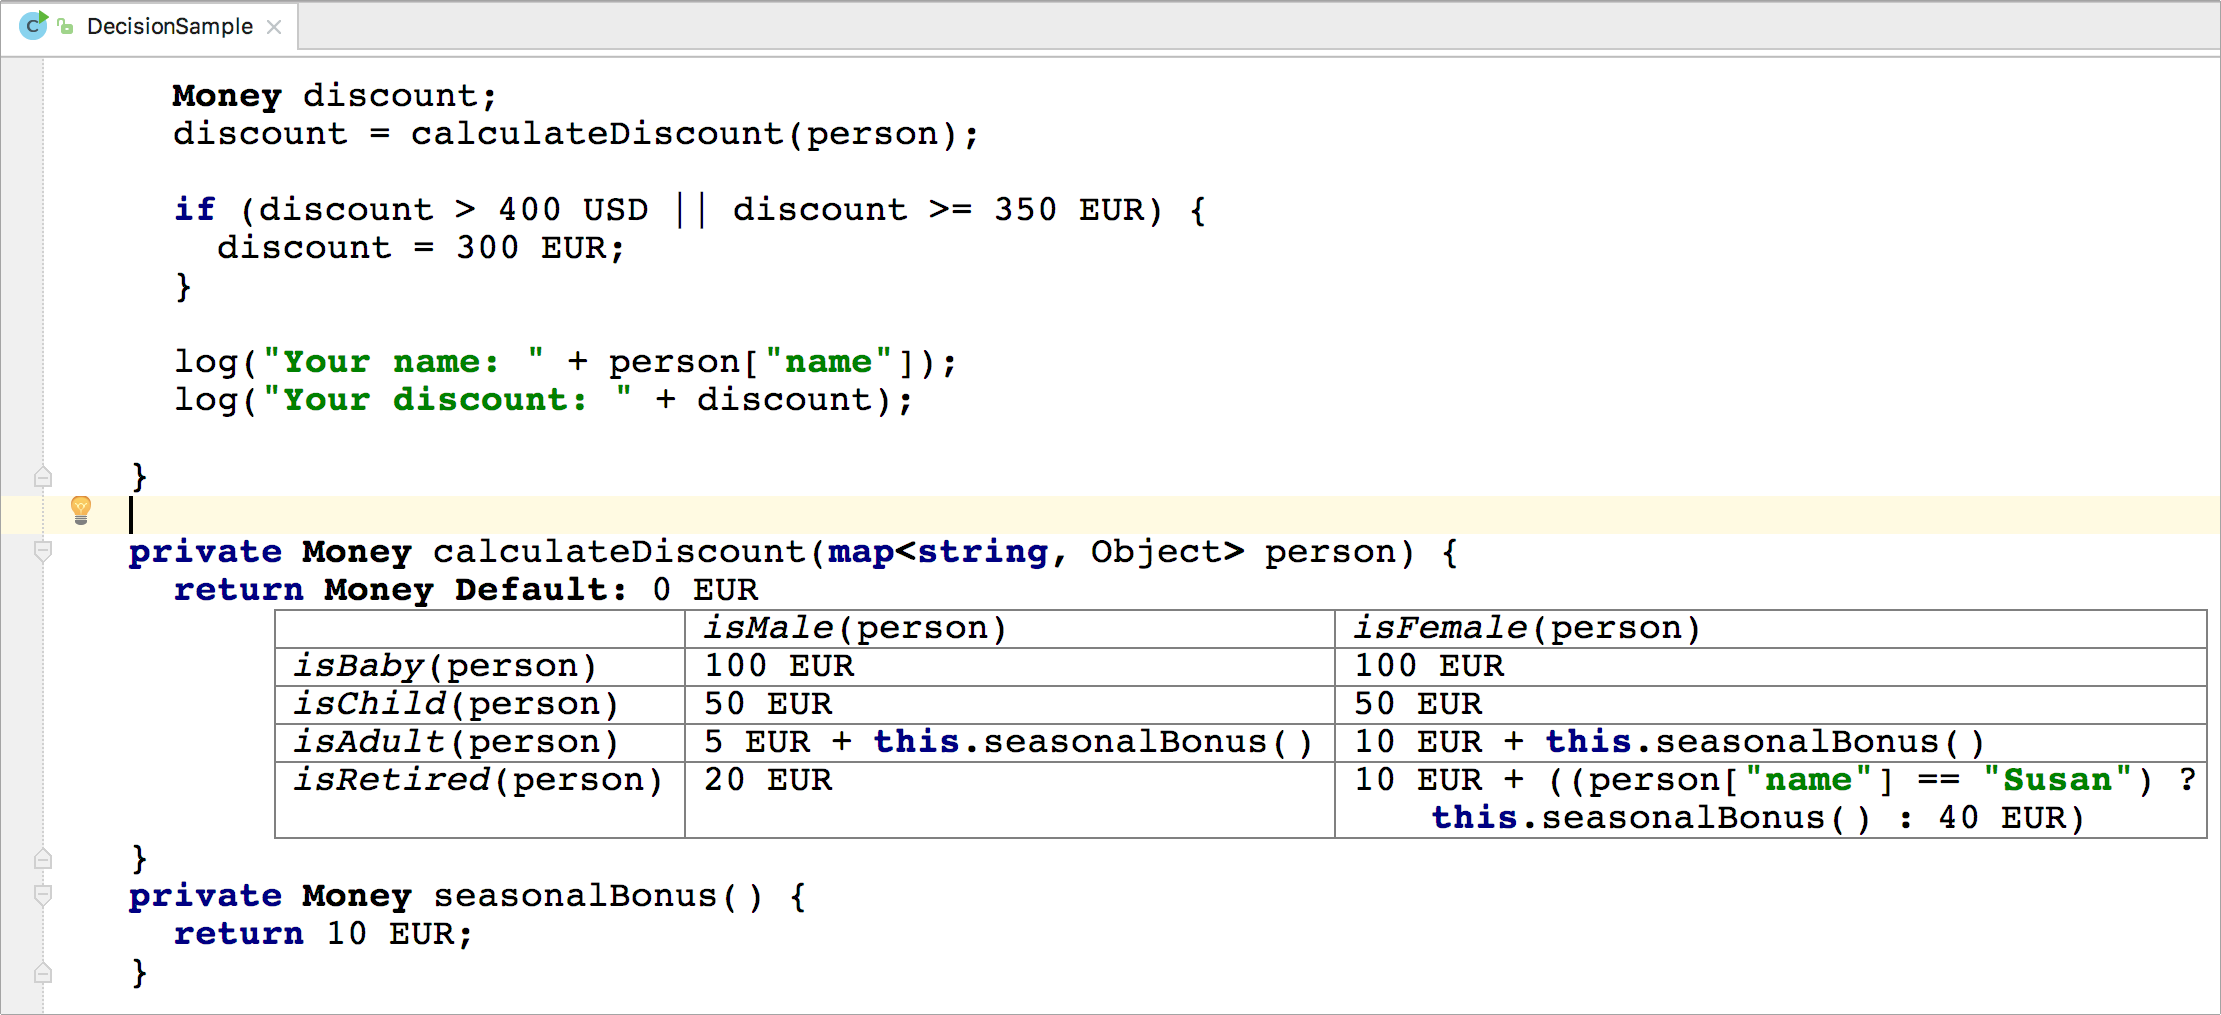
\includegraphics[width=0.48\textwidth]{images/domain-specific-languages.png}\figlabel{MpsPreview}} \hspace{0.1cm}
\subfloat[]{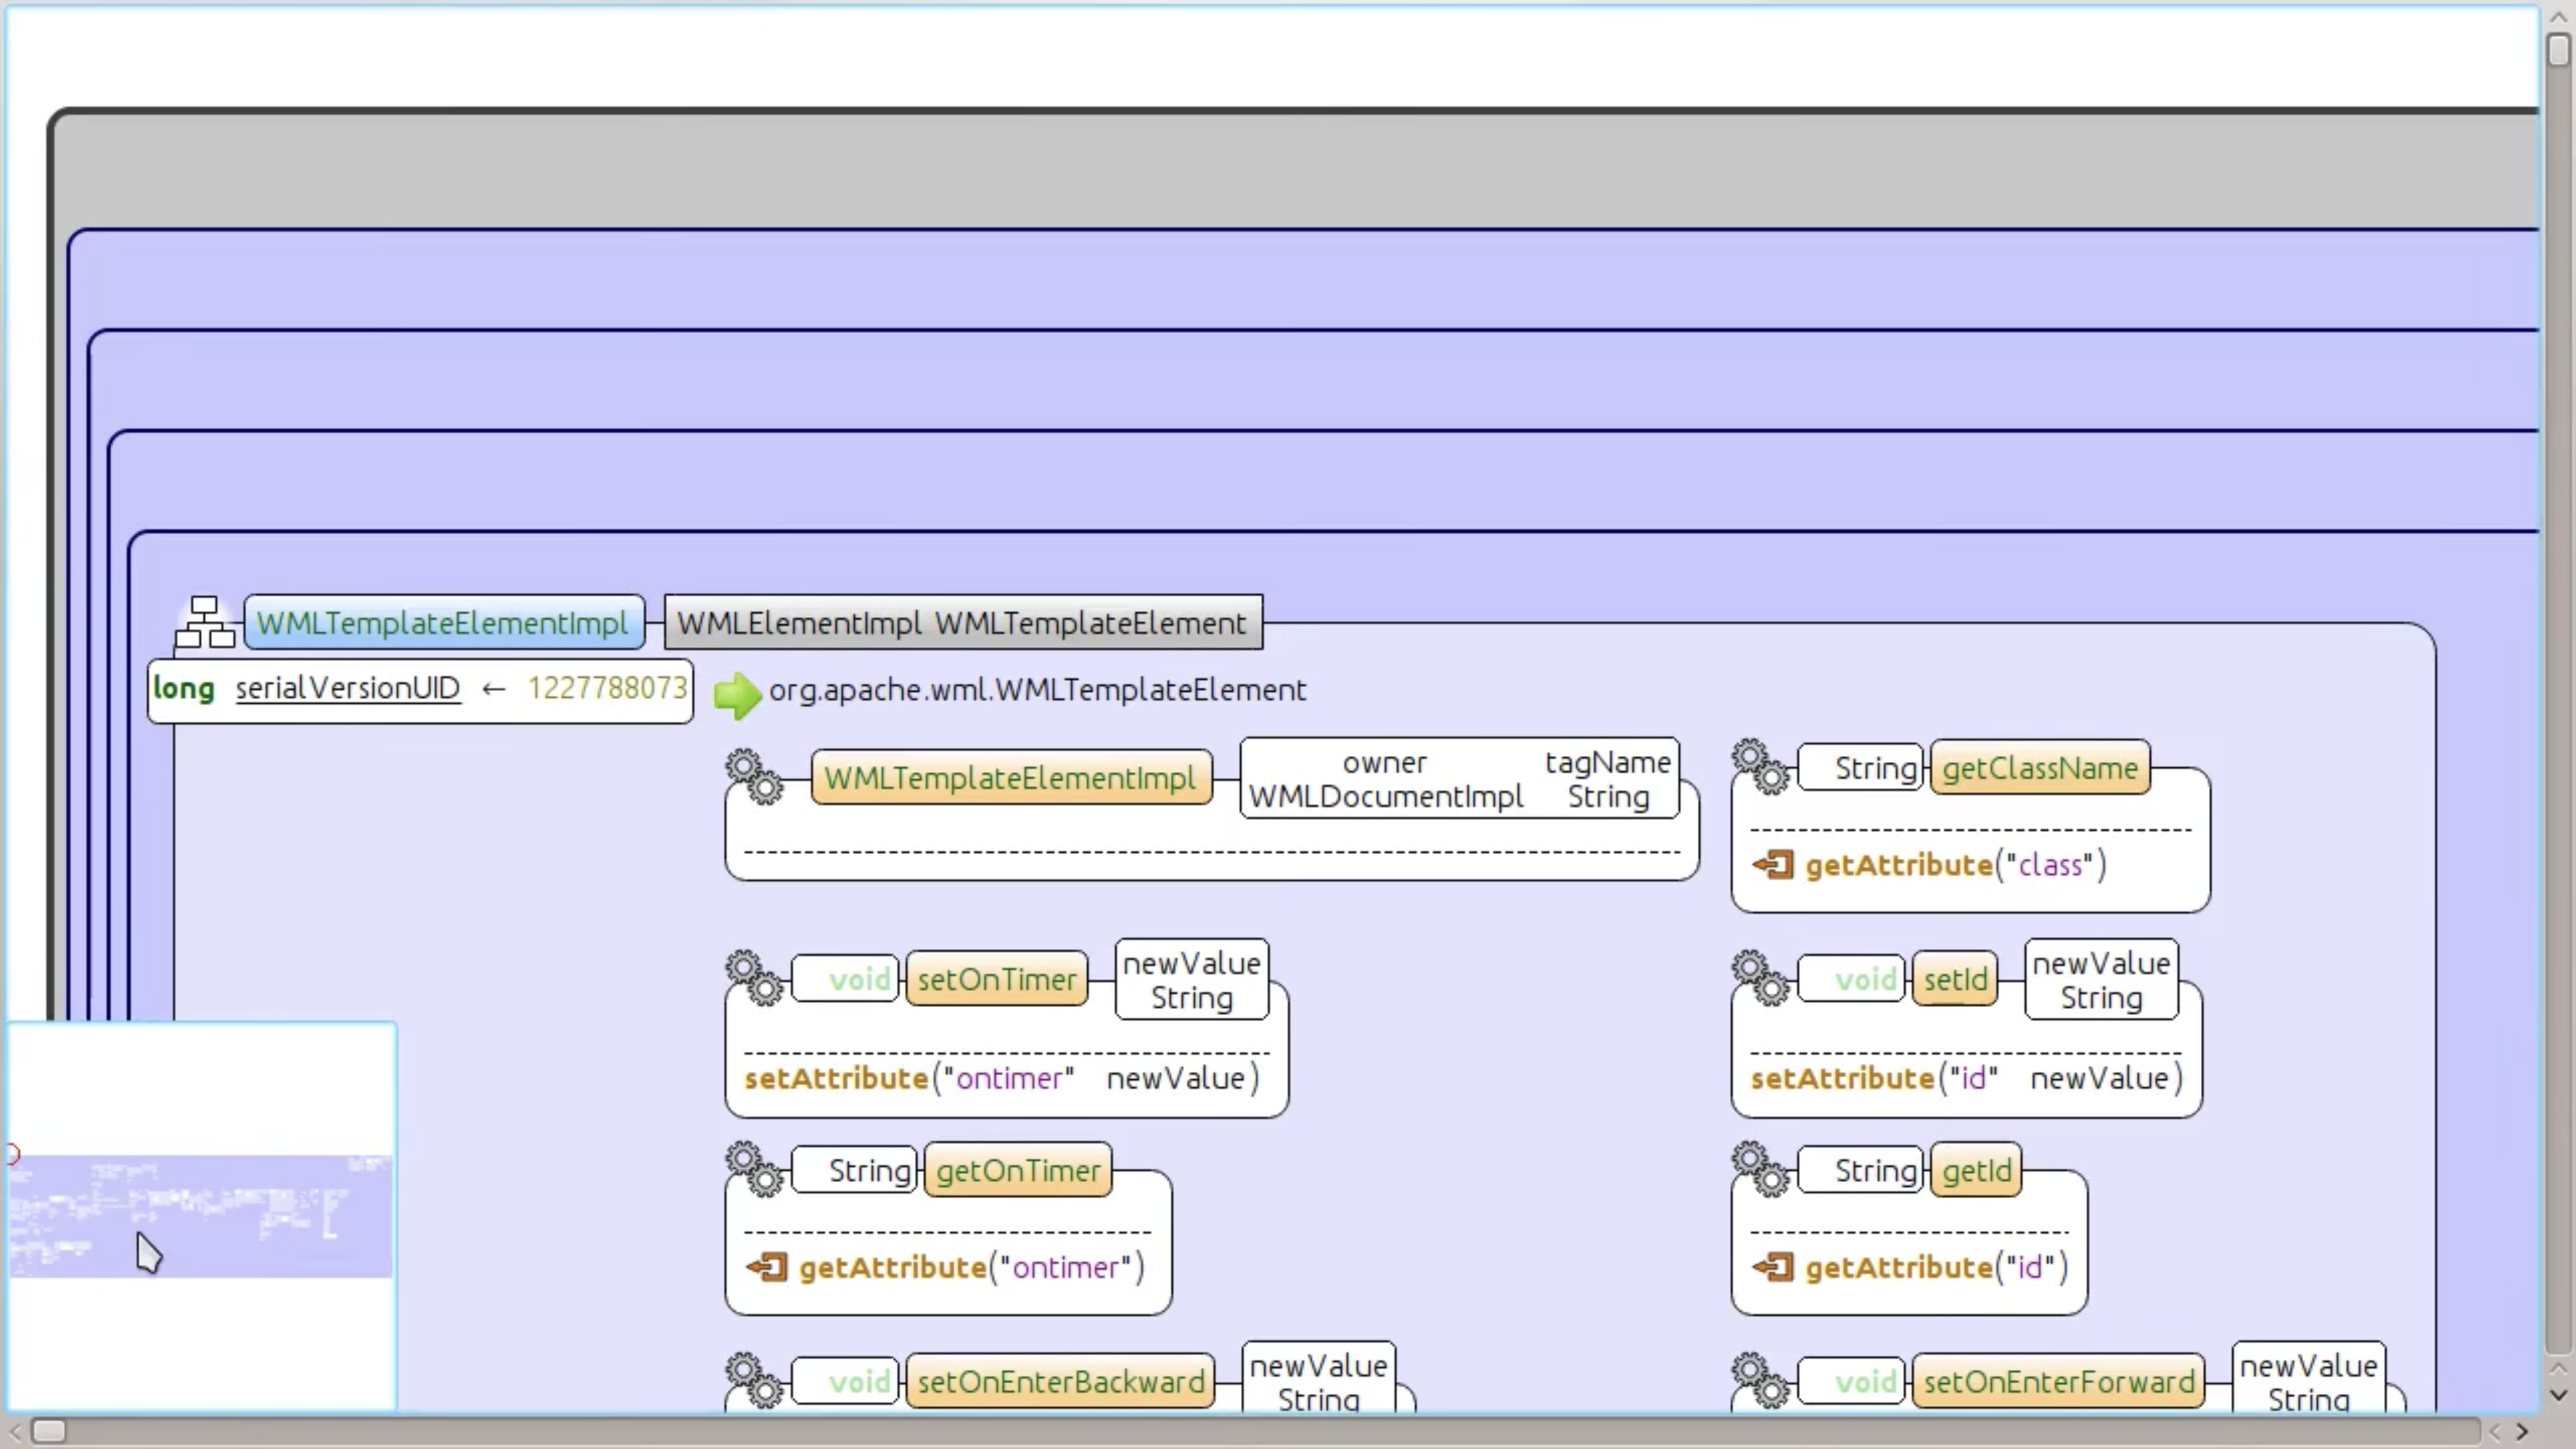
\includegraphics[width=0.48\textwidth]{images/envisionpreview.png}\figlabel{EnvisionPreview}}\hspace{0.1cm}
\caption{Examples of the editors combining code and graphical views: \emph{a)} Jetbrains MPS; \emph{b)} Envision.}  
\figlabel{RelatedEditors}
\end{figure*}

\newpage
An interesting example is the Jupyter Notebook \footnote{\url{http://jupyter.org/}} that combines live code, visualisations and explanatory text to create documents (\figref{JupyterPreview}).

For example, MPS \footnote{\url{https://www.jetbrains.com/mps/}}, makes one step forward by displaying domain entities using graphical views (e.g., editing a matrix using a table view, editing a state machine using a graph view); views are selected based structural aspects of the code. Envision\footnote{\url{http://dimitar-asenov.github.io/Envision/}}, proposed a highly scalable visual editor (\figref{RelatedEditors} \emph{(b)}).

\begin{figure}[t]
\centering

\includegraphics[width=0.78\columnwidth]{images/jupyterpreview.png}
\caption{Jupyter Notebook}
\figlabel{JupyterPreview}
\end{figure}

Playgrounds, like Swift\footnote{\url{https://developer.apple.com/swift/playgrounds}}, Scala\footnote{\url{https://github.com/scala-ide/scala-worksheet/wiki/Getting-Started}} or Eve\footnote{\url{http://witheve.com}}, give live and continuous feedback of a computation by adding graphical views next to the code. Many IDEs, when in the debugger, link the code editor with run-time objects (\eg Eclipse, IntelliJ, VisualStudio), and display views in pop-ups. IDEs like Pharo\footnote{\url{http://pharo.org}} or Squeak\footnote{\url{http://squeak.org}}, embed the code editor into the object inspector. Another category of systems provide complete graphical editors. This includes, for example, modelling frameworks, like EMF\footnote{\url{https://eclipse.org/modeling/emf/}} or VPL\footnote{\url{https://msdn.microsoft.com/en-us/library/bb483088.aspx}}, or visual languages~\cite{Citr95}.

%===================================================================================================
%===================================================================================================
%=========================================  T H E  E D I T O R   ==========================================
%===================================================================================================
%===================================================================================================

\chapter {The Moldable Editor}

\section{Overview}

\begin{figure}[t]
\centering
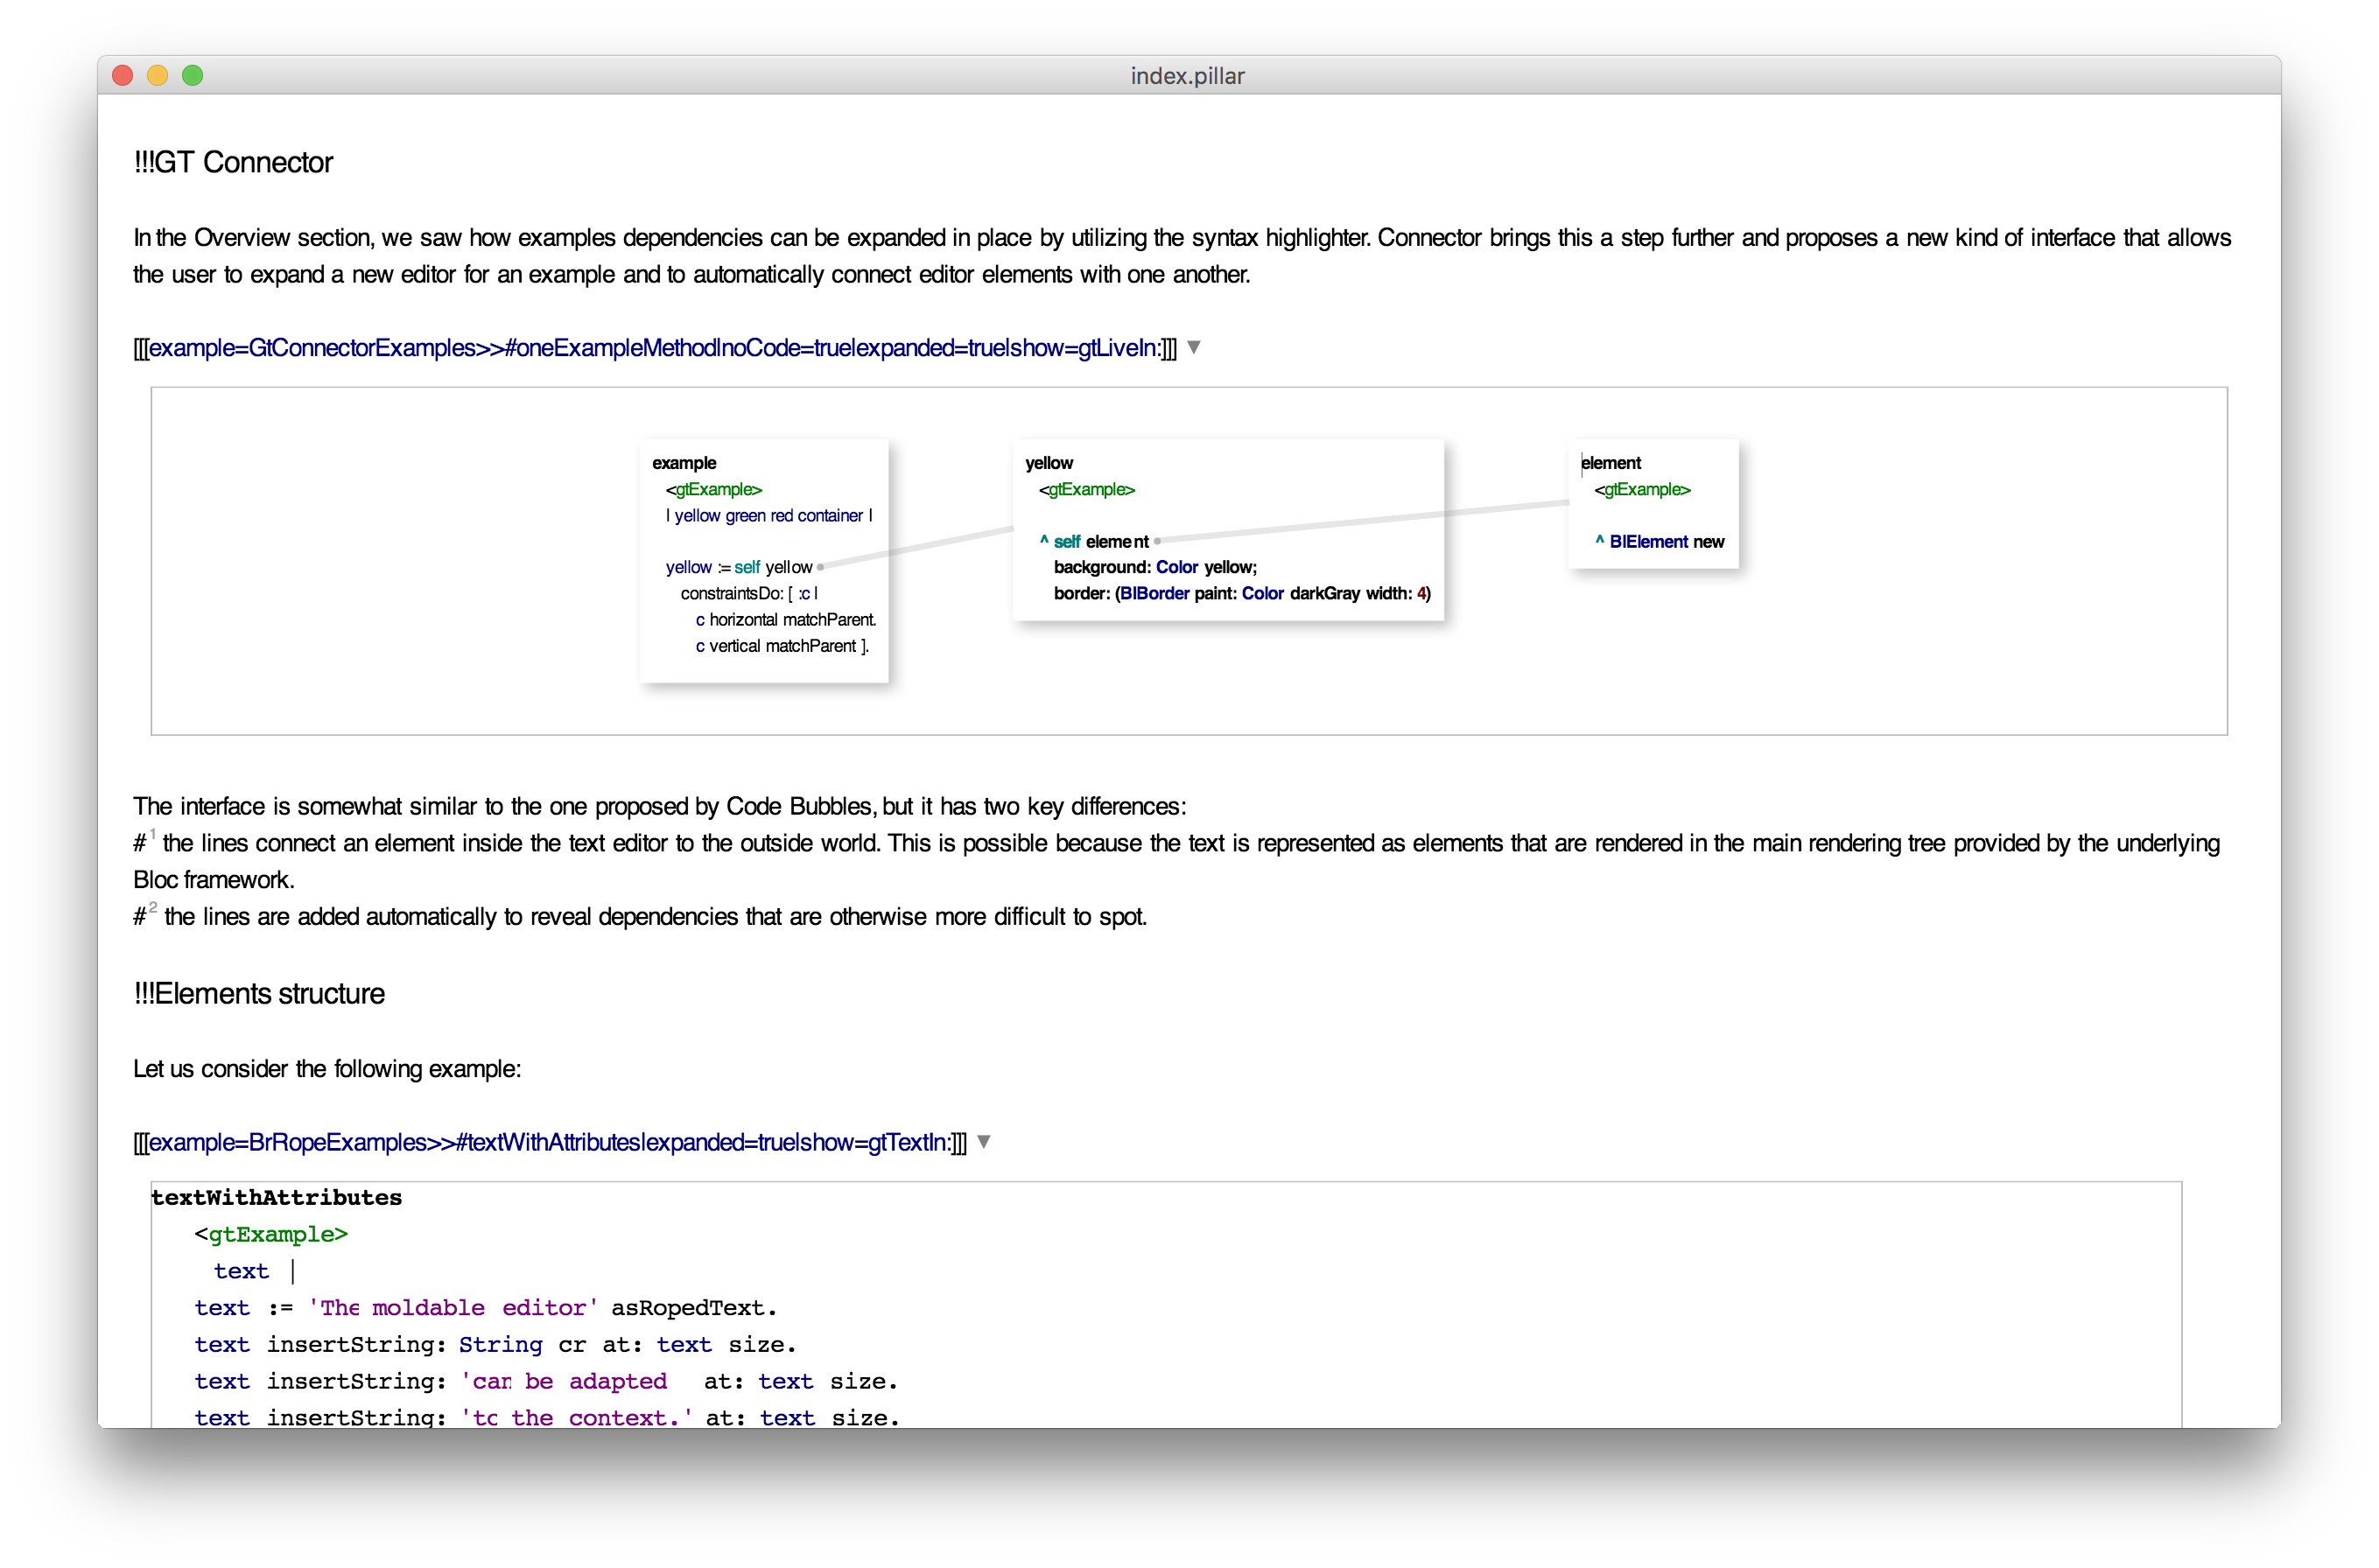
\includegraphics[width=0.87\columnwidth]{images/moldable-editor-preview.png}
\caption{The Moldable Editor}
\figlabel{TheMoldableEditorPreview}
\end{figure}

The Moldable Editor is a flexible and scalable editor designed as a single composition tree of visual elements.

One of the requirements for that type of the editor is an ability to embed visual components inside of text such that they are not deletable nor selectable. We call those elements \textit{adornments}. To unify how text and adornments are being treated, the editor also represents pieces of text as visual elements, thus completely removing a gap between embedded graphical components and text which is what allows us to have a single composition tree.

The basis and foundation of the editor is a text model. An interesting aspect of that text model is the fact that it is data structure independent. It allows us to implement different types of text types, for example \ct{SubText}, that can creates a subset of existing text within an interval, or \ct{SpanText}, that represents a uniform piece of text where all characters have identical attributes. From the text editor's perspective there is no difference between those types of text, the interaction happens through a clear \ct{Text} API. More about text model can be found in Section \ref{TextModelSection}.

When talking about text model we should not forget about text style, which is defined by a set of text attributes. Those attributes can be applied on the text manually with the help of corresponding text model API or created automatically by text stylers. Text stylers play an important role in syntax highlighting used by code editor.  Even more important role they play in the moldable editor as they are used to add \textit{adornment} attributes and hence provide a nice way to plug-in custom behaviour in the editor. Text stylers take context into account which is essential for creation of context-aware development tools. In order for the editor to be fast and responsive, long and time consuming operations such as text parsing and styling should happen in a parallel background thread. It is in fact a non-trivial task, since users are able to perform text modification operations while a styler applies attributes on a text that is being modified. In Section \ref{TextStyleSection} we talk more about problems and difficulties related to text styling and introduce a solution that is currently implemented in and used by the moldable text editor.

In order for the moldable editor to be scalable, it should split text into logical segments and render only those ones that are currently visible. A segment can be a page, a paragraph or a line. In the current implementation, the text editor creates line segments with the help of a line segment builder. The process of splitting text into segments is trivial, however keeping segments in sync with the text model after modification such as insertions and deletions is a difficult part and very error-prone. Once segments are built they should be rendered as visual elements and displayed within the editor. The way it happens is similar to how modern scrolling lists work, for example \textit{FastTable} in Pharo, \textit{RecyclerView}\footnote{\url{https://developer.android.com/reference/android/support/v7/widget/RecyclerView.html}} in Android or \textit{UITableView}\footnote{\url{https://developer.apple.com/documentation/uikit/uitableview}} in iOS. Segments are held by a data source object which knows how segments should be represented. It is also responsible for binding a segment model to its visual representation. In most cases a logical segment consists of multiple segment pieces, for example a line segment consists of words - text pieces separated by a white space. White space itself is also a piece within a line segment. A structure of the segment and its visual part is explained in more details in Section \ref{SegmentsAndRenderingSection}.

%------------------------------------------------------------------------------------------------------------------------------------------------------------------------------
%----------------------------------------------------------------------------- T E X T   M O D E L ---------------------------------------------------------------------%------------------------------------------------------------------------------------------------------------------------------------------------------------------------------
\section{Text Model}
\label{TextModelSection}
\begin{figure}[t]
\centering
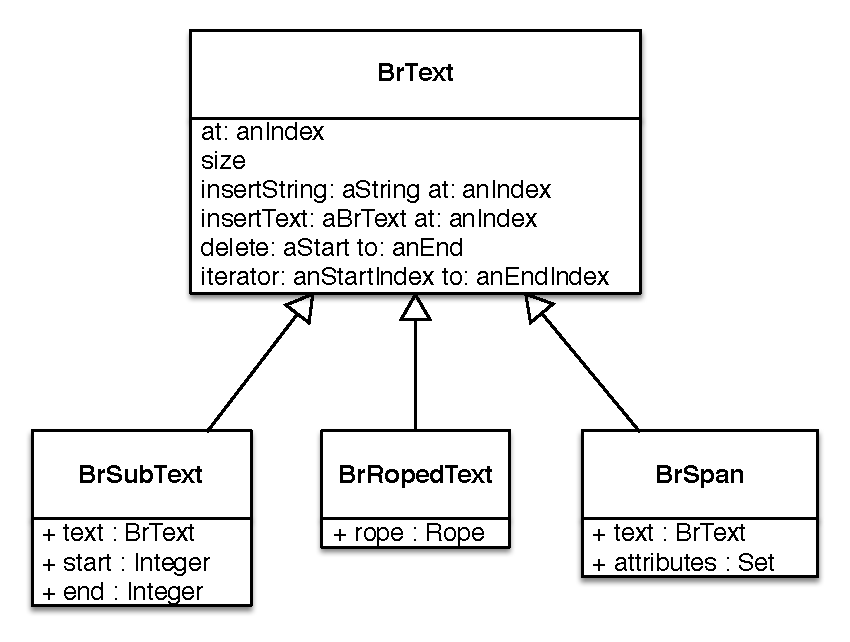
\includegraphics[width=0.65\columnwidth]{figures/text-model-uml.pdf}
\caption{The UML class diagram of Text Model}
\figlabel{TextModelUml}
\end{figure}

To display and edit text, an editor requires a text model that provides text modification and enumeration API. In a context of text editor by \textit{Text} we understand an object that consists of a collection of characters with a set of attributes applied on those characters and a number of API methods to support text modifications such as \ct{insert:} or \ct{delete:}. Additionally, text should play a role of sequenceable and indexable collection, allowing users to iterate over all characters in a natural ordered way. Being indexable is an essential property of a text model, since text stylers require text to have characters accessible by index. Code parsers create an \textit{AST} which consists of nodes bound to original text with the help of integer intervals in a form of a \textit{[from, to]} tuple. Those intervals are later used by a text styler to apply attributes on a piece of text within those intervals.

%------------------------------------------------------------------------------------------------------------------------------------------------------------------------------
%------------------------------------------------------------------ T E X T   D A T A   S T R U C T U R E S ------------------------------------------------------%------------------------------------------------------------------------------------------------------------------------------------------------------------------------------
\section{Text data structures}

To be considered scalable the moldable editor should be able to manipulate large pieces of text that consist of millions of characters and sometimes even more. It means that choosing an appropriate data structure for storing text is crucial. After searching for a data structure to be used by a text model we realised that there is no a "silver bullet" data structure that is memory efficient, has the fastest random access and modification operations. Instead, it turned out that depending on a context and a way text editor will be used it may be important to be able to select one or another data structure based on its properties. That is why a text model of the moldable editor is data structure independent and only defines a public API. In order for it to be used by a text editor developers should create concrete implementations of that API backed up by the data structure of choice. In the following sub-sections we look at different data structures being used by text editors and compare them.

\subsection{Pharo}

In Pharo there already exist two text models based on different data structures: one is \ct{Text} which is used by both \textit{Morphic} and \textit{Rubric} text editors, and \ct{TxModel} used by \textit{TxText editor}.
\subsubsection*{Rubric}

\begin{figure}[ht]
\centering
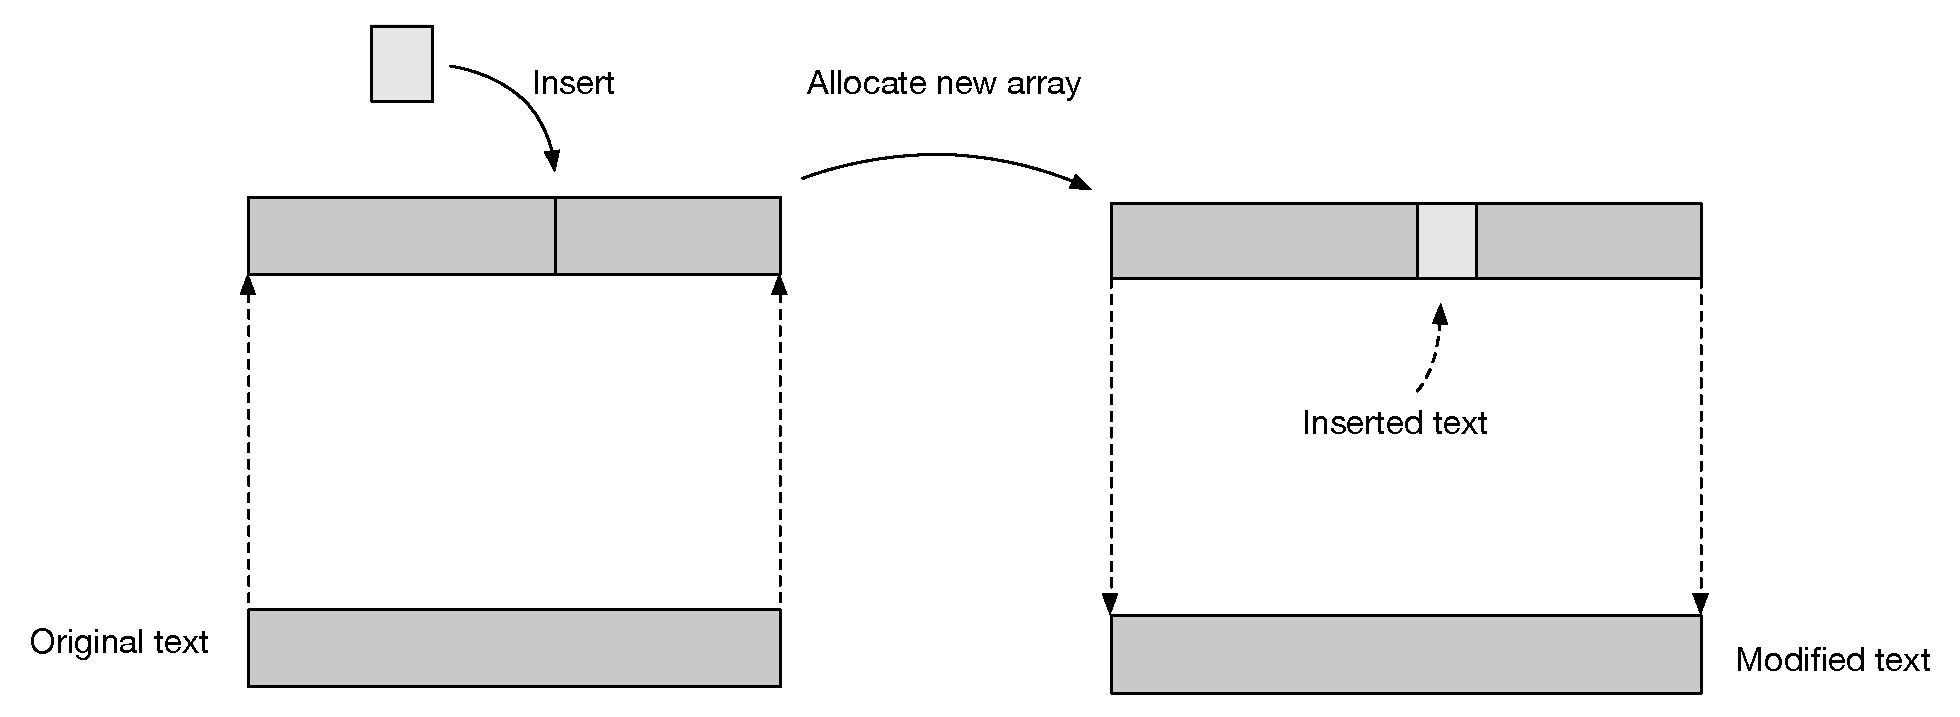
\includegraphics[width=0.85\columnwidth]{figures/data-structure-array.pdf}
\caption{The array method}
\figlabel{ArrayText}
\end{figure}

\ct{Text} is a default Pharo text model. It stores a collection of characters and a set of attributes separately. Characters are represented with the help of \ct{ByteString} which is nothing else than an immutable array of characters. It means that every text modification such as insertion or deletion requires text model to allocate and copy the whole array while replacing a subsequence of characters with a requested one as shown on \figref{ArrayText} The algorithm of text modifications is in this case linear time and requires massive memory copy operations, which becomes unacceptably slow when text size growths over hundreds of thousands of characters. In fact, array is the worst data structure for text sequences  \cite{crowley1998data}.

\subsubsection*{TxText}

\begin{figure}[ht]
\centering
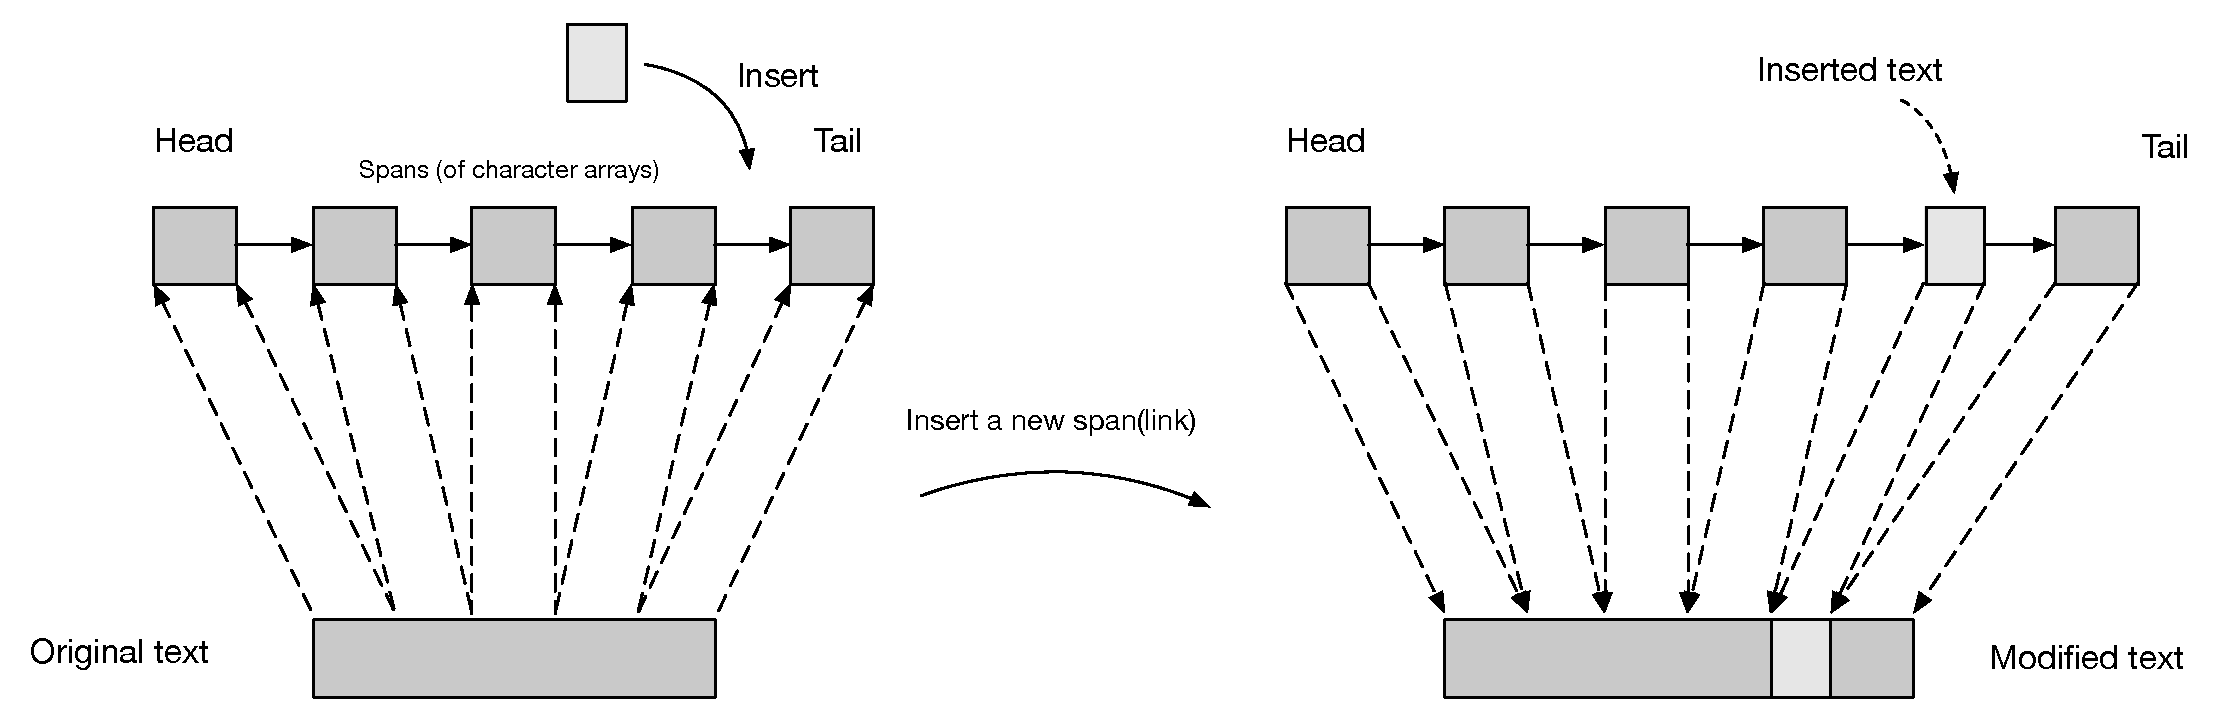
\includegraphics[width=0.85\columnwidth]{figures/data-structure-linked-list.pdf}
\caption{The linked list method}
\figlabel{LinkedListText}
\end{figure}

\ct{TxModel} is a central class representing a text in the \textit{TxText editor}. Internally is stores character sequences as a double-linked list of spans that consists of an actual text content. A linked list is considered to be an extreme as opposed to an array method of storing text. While insertions and deletions in a linked list are fast and easy, it is only indexable in a linear time which makes styling one of the slowest among all other text data structures \cite{crowley1998data}.

\subsection{Atom}

Atom\footnote{\url{https://atom.io/}} text editor uses a memory-efficient data structure similar to a Piece Table \cite{atomblog2018}. Piece table is a data structure based on two buffers, one of which represents original read-only text while the second one stores all modifications done to that text. All essential operations are performed with an adequate performance and some of them can  be efficiently improved by using cache. Piece table is considered to be the data structure of choice for a text editor \cite{crowley1998data}.

\newpage
\subsection{Emacs}

Emacs\footnote{\url{https://www.gnu.org/software/emacs/}} is based on a Gap Buffer, a data structure a little more complex as array but much more efficient \cite{crowley1998data}. The idea behind the gap buffer is simple, the whole text is stored in a large buffer that contains a gap at a cursor location or at a place where editing operations happen. Of course, this means that the gap must first be moved to the locus of the insertion or deletion. When the gap is correctly positioned editing operations are very efficient since the size of a buffer is small. However, the first editing command in one part of a large buffer, after previously editing in another far-away part, sometimes involves a noticeable delay \cite{emacs2017}. A delay happens because to move a gap the whole buffer that stores the text has to be reallocated and memory to be moved.

\begin{figure}[ht]
\centering
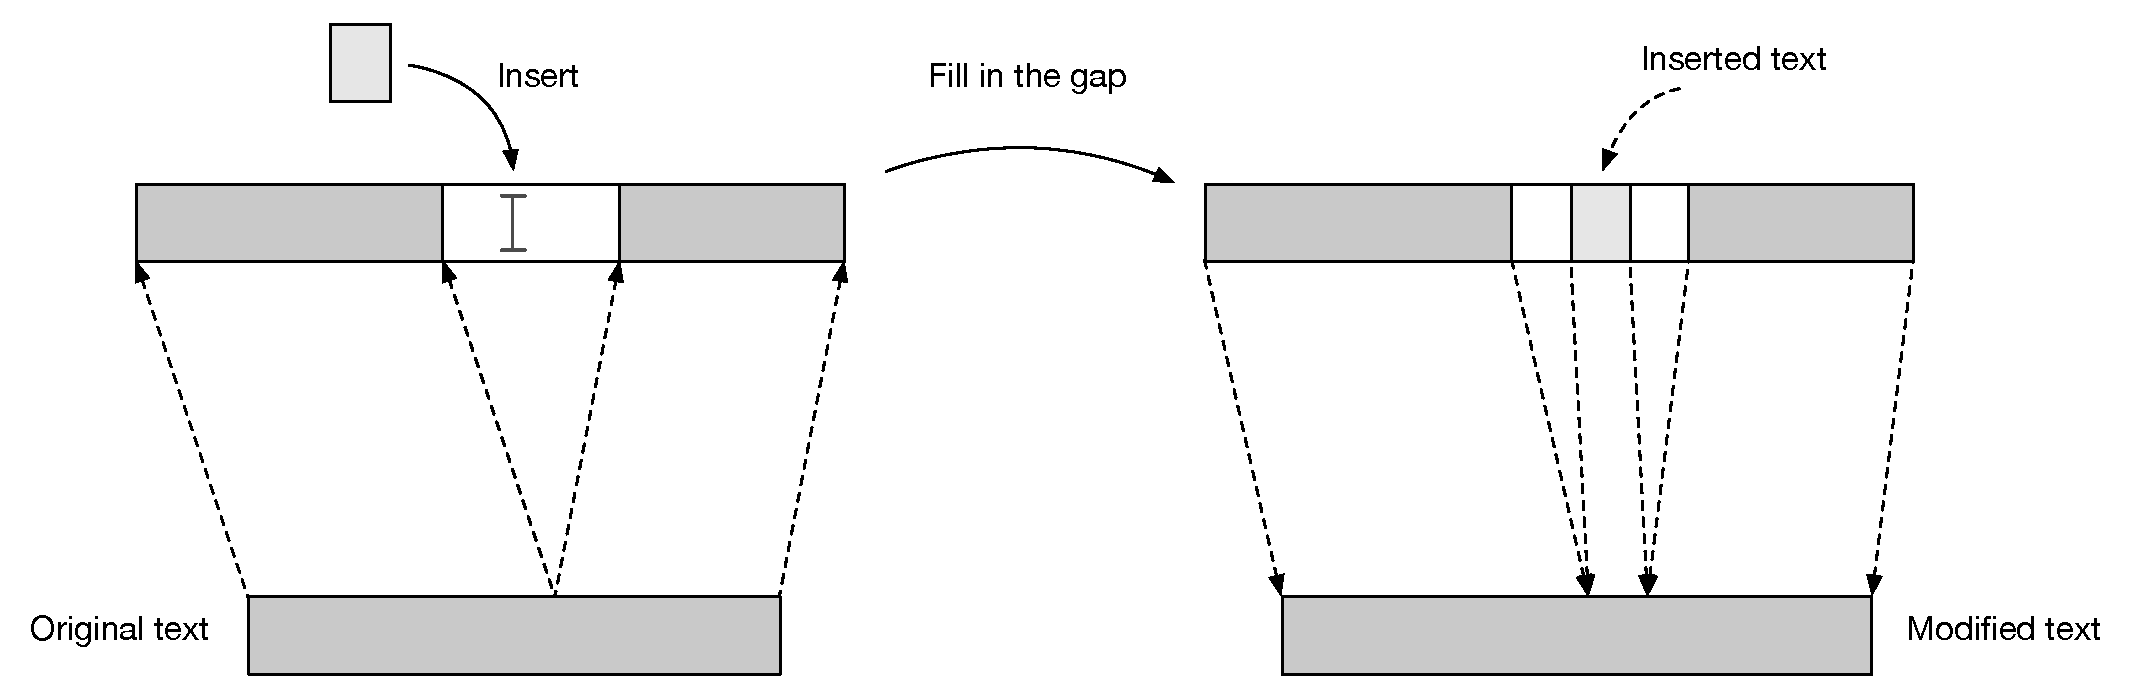
\includegraphics[width=0.75\columnwidth]{figures/data-structure-gap-buffer.pdf}
\caption{The gap buffer method}
\figlabel{GapBufferText}
\end{figure}

\figref{GapBufferText} shows the workflow of an insertion operation with assumption that a gap buffer (white block) is already moved to the cursor location. 

\subsection{Rope}

An alternative to array or buffer-based data structures is Rope. Rope is a tree of concatenation nodes representing character strings. \cite{boehm1995ropes} In addition to concatenation nodes, depending on implementation, rope may include subset nodes, reverse nodes or other custom types of nodes. Rope allows text editors to manipulate large pieces of text and makes text operations such as random access, insertion and deletion very efficient. However, to maintain high efficiency rope must be re-balanced otherwise it may loose its binary search tree properties and operations become inefficient.

If all operations are implemented in a non-destructive way, rope becomes a persistent data structure. To enforce that, any modification should return a new node instance with applied changes. A root node of the returned rope, in this case, does not necessarily have the same type as the one that was modified. From a text editor perspective, persistence makes it easier to implement undo/redo commands and helps to prevent multithreading issues when it comes to text styling.

One of the main disadvantages of the Rope is its implementation complexity and high possibility of bugs as a consequence. Compared to other common text data structures, rope requires more memory space to store its tree structure. In languages without garbage collector, maintaining node references may be a tedious task and may lead to memory leaks.

Due to its disadvantages, Rope didn't become a traditional and commonly used data structure to be used in text editors. For that reason it was not possible to see Rope in action, in a contrast to gap buffer or piece table that are nowadays used by modern and popular text editors. Its rare and complex nature, tree structure and possible object oriented implementation as also the existence of a garbage collector in Pharo made Rope a data structure of choice for the Moldable Editor.

\subsubsection*{Collection node}
One of the main building blocks of the Rope is a \textit{collection} node (\figref{RopeCollectionNode}). It is nothing else than a fixed buffer of characters of a limited length.

\begin{figure}[h]
\centering
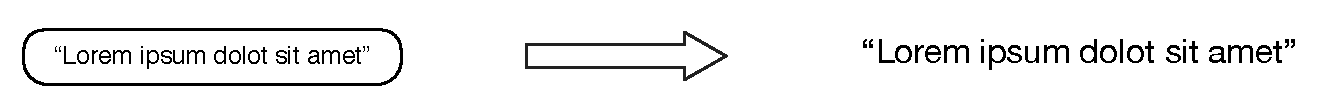
\includegraphics[width=0.80\columnwidth]{figures/data-structure-rope-collection.pdf}
\caption{Collection node}
\figlabel{RopeCollectionNode}
\end{figure}
If a total length of two collection nodes that are being merged exceeds a predefined limit, a result would be a \textit{concatenation} node consisting of those collection nodes.

\subsubsection*{Concatenation node}

\textit{Concatenation} node has a central role in the structure of the Rope. Similar to the binary search tree it knows its \textit{left} and \textit{right} child nodes.

\begin{figure}[h]
\centering
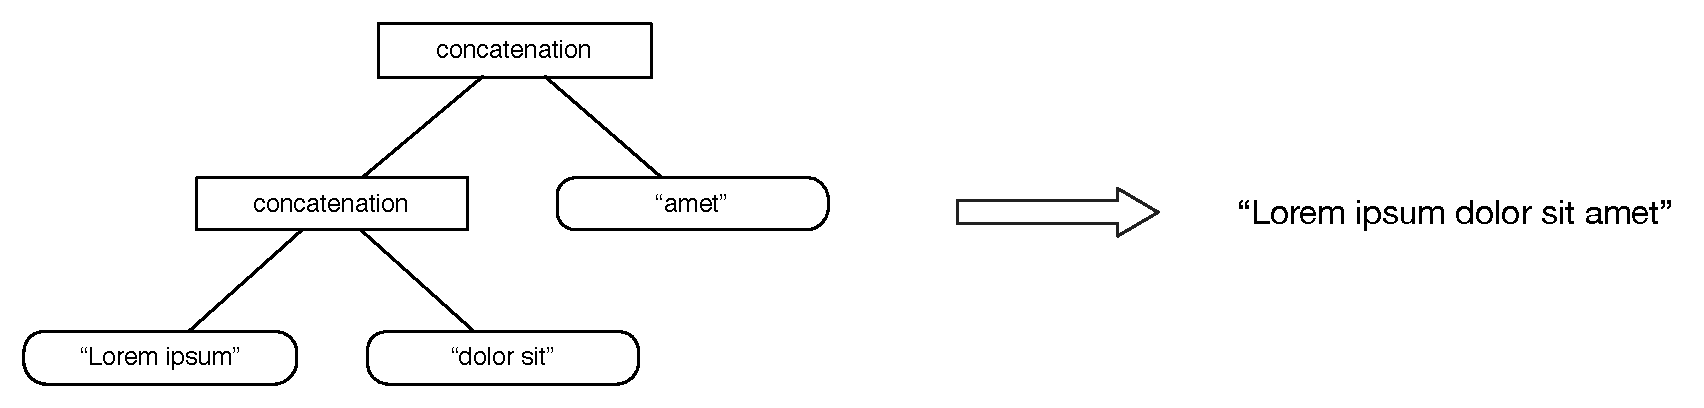
\includegraphics[width=0.95\columnwidth]{figures/data-structure-rope-concatenation.pdf}
\caption{Concatenation node}
\figlabel{RopeConcatenationNode}
\end{figure}

If a total length of two ropes being concatenated is lower then a predefined limit, then instead of creating a concatenation node, they can be merged into a single \textit{collection} node which allows Rope to be more memory-efficient and reduce amount of intermediate nodes.

\newpage
\subsubsection*{Subset node}

An ability to get a substring defined by an index interval plays in important role for the text editor, for example in case of \textit{copy} or \textit{cut} commands. It can be implemented by introducing a \textit{subset} node that is a wrapper around other rope node with additional \ct{start} and \ct{end} attributes.

\begin{figure}[h]
\centering
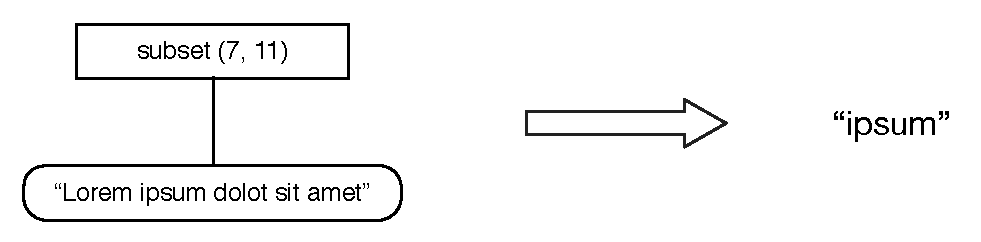
\includegraphics[width=0.80\columnwidth]{figures/data-structure-rope-subset.pdf}
\caption{Subset node}
\figlabel{RopeSubsetNode}
\end{figure}

\subsubsection*{Attribute node}

As it is mentioned in Section \ref{TextModelSection} \textit{Text} is not only a collection of characters but a set of associated attributes such as font size, text foreground or text style. Traditionally, attributes are stored in a separate data structure along a text sequence. For example \textit{Rubric} text model allocates a dedicated \textit{RunArray} of the same length as text itself, where every item is an array of attributes that corresponds to the character with identical index as shown on \figref{RubricTextAttributesArray}.

\begin{figure}[h]
\centering
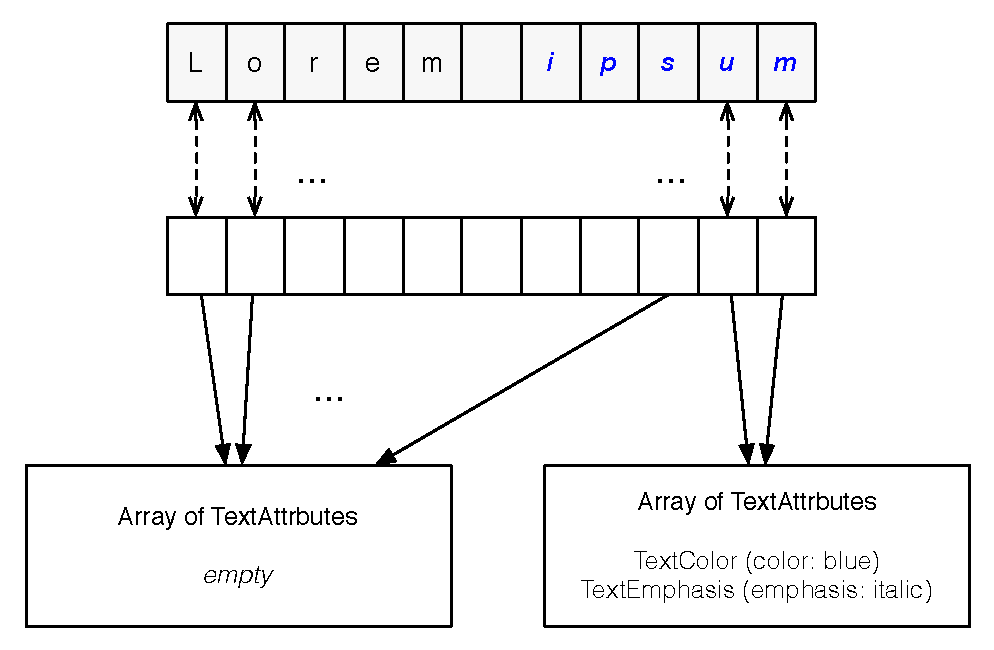
\includegraphics[width=0.75\columnwidth]{figures/text-attributes-array.pdf}
\caption{Text attributes structure of the Rubric text model}
\figlabel{RubricTextAttributesArray}
\end{figure}

Instead of creating a separate data structure for text attributes, it is possible to incorporate it directly inside of the rope hierarchy by introducing a new \textit{attribute} node. Attribute node is a wrapper around any rope node and it additionally stores a set of attributes that should be applied on that node as shown on \figref{RopeAttributeNode}. It makes it possible to apply attributes on the whole rope by only wrapping it in a single object, which consumes less space compared to traditional solutions as they have to allocate at least the same amount of memory as consumed by the text sequence.

\begin{figure}[h]
\centering
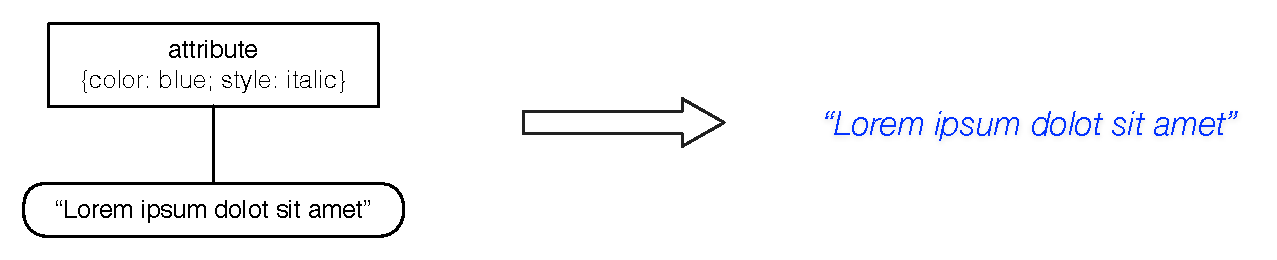
\includegraphics[width=0.95\columnwidth]{figures/data-structure-rope-attribute.pdf}
\caption{Attribute node}
\figlabel{RopeAttributeNode}
\end{figure}

Additionally, attribute node makes it easier and more efficient to iterate over text \textit{spans}, pieces of text where all characters have the same attributes. This iteration is necessary during the rendering or text measurement process, where every span has to be rendered or measured separately, since underlying 2D graphics libraries only capable of rendering text sequences of the same pre-set style.\cite{skiaText}\cite{cairoText}

%
%\begin{figure*}[h]
%\centering
%\subfloat[]{
\includegraphics[width=0.32\textwidth]{images/rope-tree-1.png}\figlabel{RopeTree1}}\hspace{0.1cm}
%\subfloat[]{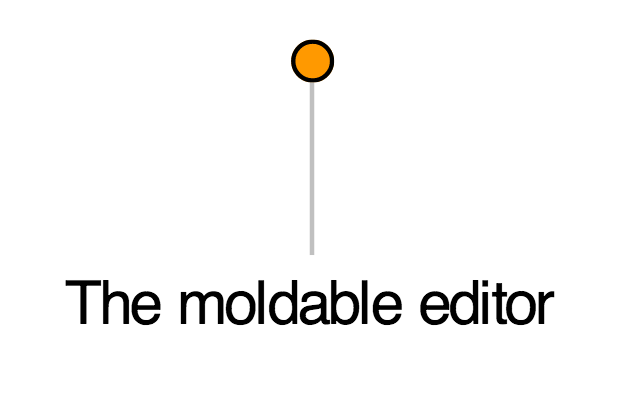
\includegraphics[width=0.32\textwidth]{images/rope-tree-2.png}\figlabel{RopeTree2}}\hspace{0.1cm}
%\subfloat[]{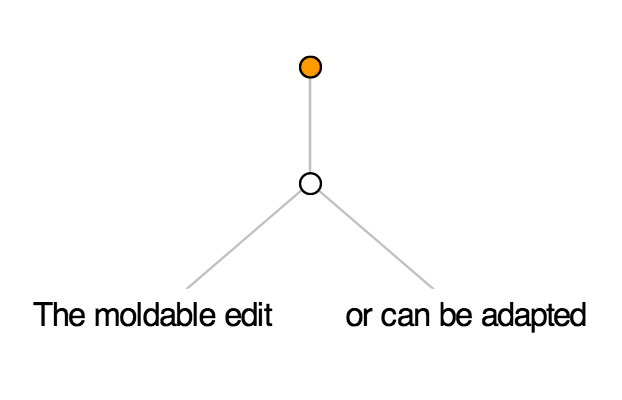
\includegraphics[width=0.32\textwidth]{images/rope-tree-3.png}\figlabel{RopeTree3}}
%\subfloat[]{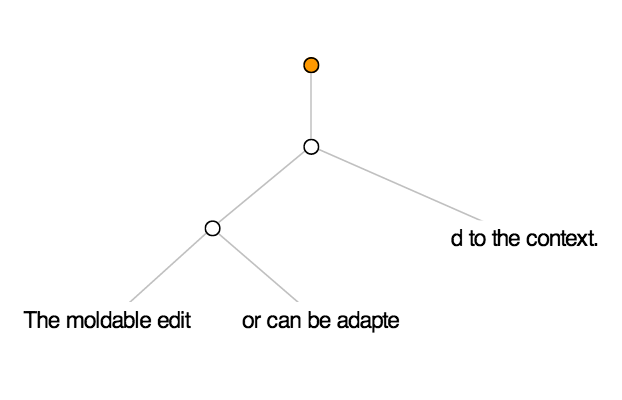
\includegraphics[width=0.32\textwidth]{images/rope-tree-4.png}\figlabel{RopeTree4}}\hspace{0.1cm}
%\subfloat[]{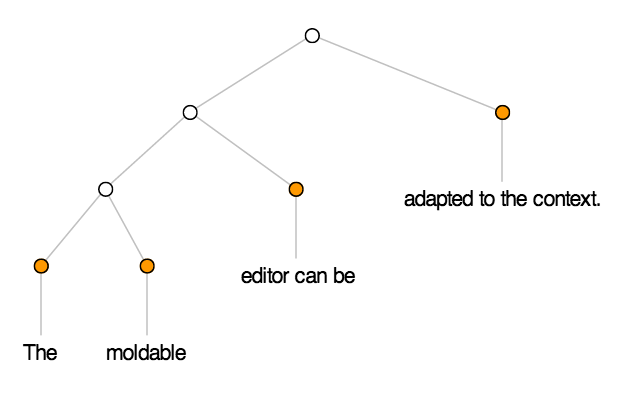
\includegraphics[width=0.32\textwidth]{images/rope-tree-5.png}\figlabel{RopeTree5}}\hspace{0.1cm}
%\subfloat[]{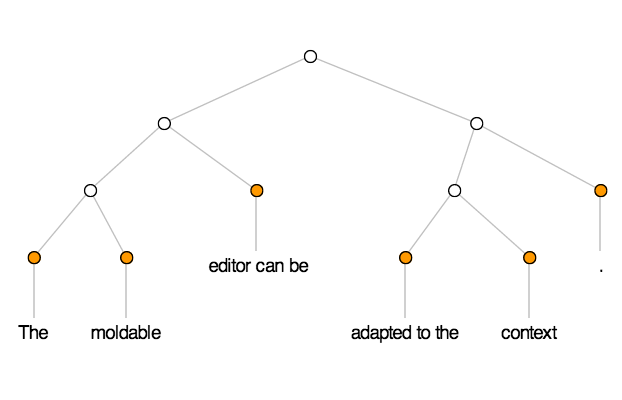
\includegraphics[width=0.32\textwidth]{images/rope-tree-6.png}\figlabel{RopeTree6}}
%\subfloat[]{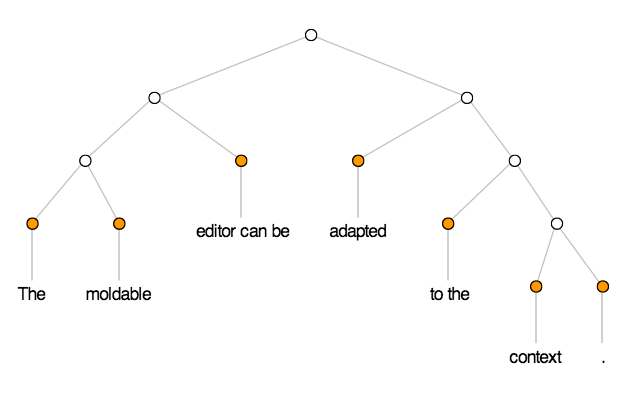
\includegraphics[width=0.32\textwidth]{images/rope-tree-7.png}\figlabel{RopeTree7}}\hspace{0.1cm}
%\caption{Three different ways to display the code of a method: \emph{a)} the standard Pharo Transcript; \emph{b)} replacing the data parameter using two distinct views; \emph{c)} replacing the results of several intermediary computations.}  
%\figlabel{RopeTree}
%\end{figure*}

\subsubsection*{Implementation}

\figref{RopeUml} shows the class hierarchy of the rope nodes as it is implemented in the Moldable Editor.

\begin{figure}[h]
\centering
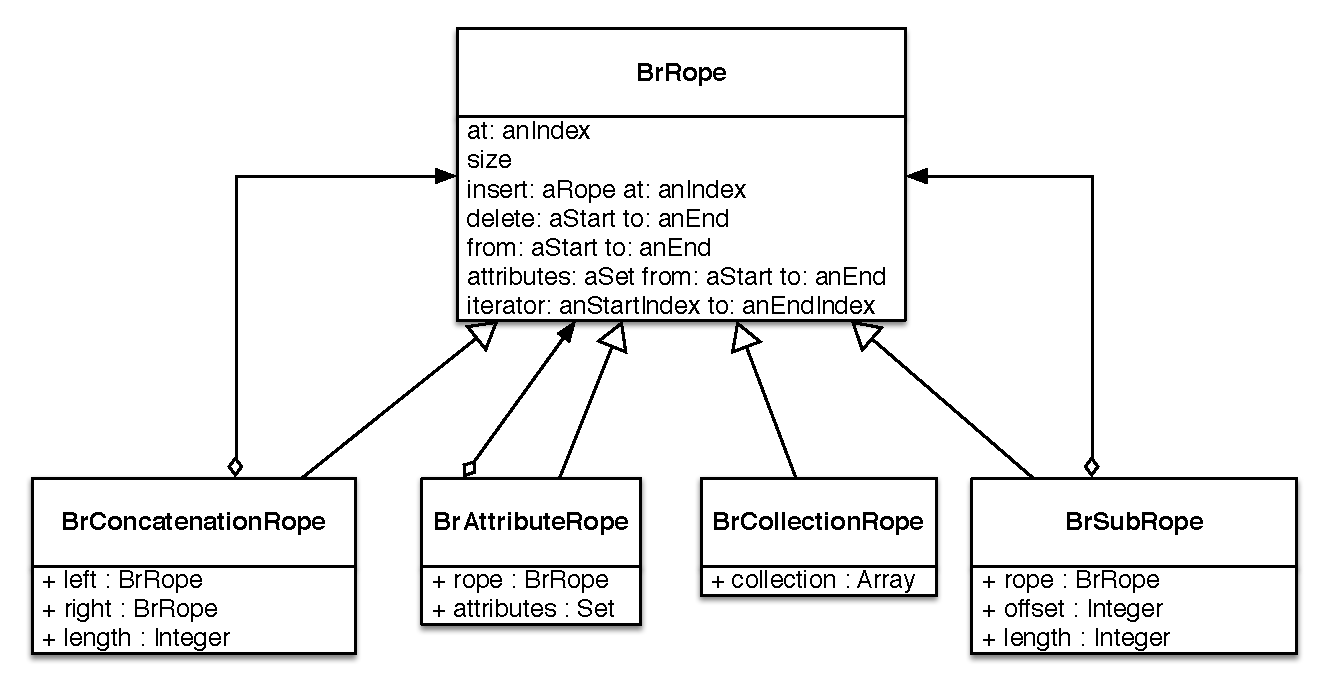
\includegraphics[width=0.8\columnwidth]{figures/rope-uml.pdf}
\caption{UML class diagram of the Rope hierarchy}
\figlabel{RopeUml}
\end{figure}



%------------------------------------------------------------------------------------------------------------------------------------------------------------------------------
%--------------------------------------------------------------------------- T E X T   S T Y L E ------------------------------------------------------------------------%------------------------------------------------------------------------------------------------------------------------------------------------------------------------------
\newpage
\section{Text style}
\label{TextStyleSection}

Text styling and syntax highlighting play an important role in the editor and should be scalable and responsive. That is why, performing styling or syntax highlighting operations in a parallel thread is the only viable option. Unfortunately, it brings its own problems and difficulties such as thread safety and text synchronisation. One of the main problem is the fact that original text can be changed during styling process. Assume the code from the \lstref{NumberOdd} and imagine we would like to style \ct{false} keyword with a style corresponding to Smalltalk pseudo-variables.

\begin{minipage}[h]{0.95\textwidth}
\begin{lstlisting}[language=Smalltalk, caption={Implementation of the \textit{\#odd} testing method from the \textit{Number} class},captionpos=b, label={lst:NumberOdd}]
odd
	"Answer whether the receiver is an odd number."

	^self even == false
\end{lstlisting}
\end{minipage}

An object responsible for styling of a source code is called \textit{syntax highlighter}. It can be implemented as a visitor of the abstract syntax tree (AST) of that source code. Leaf AST nodes know their \ct{start} and sometimes \ct{stop} positions (\figref{NumberOffFalseAstNode}) within original source code. They can be used by a syntax highlighter to apply text attributes on a text within \textit{Interval}  of that node. In our example that node interval equals to \ct{(70 to: 74)}. The problem can occur if code gets changed after computation of its AST but right before attributes are applied on the text. For example if a user would delete any character from a source code, an interval \ct{(70 to:  74)} would be no more valid, because an overall length of that source code is 73 which leads to \ct{SubscriptOutOfBounds} exception.

\begin{figure}[h]
\centering
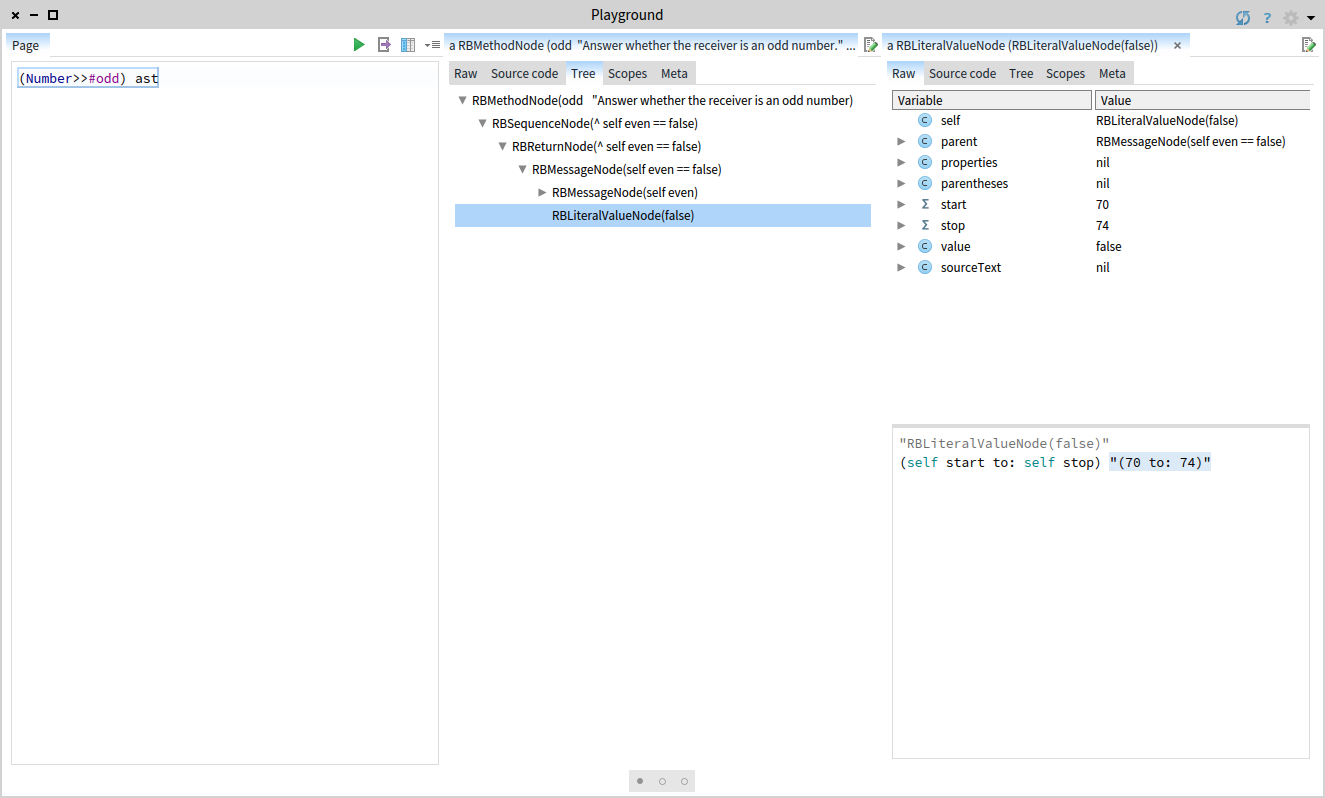
\includegraphics[width=0.8\columnwidth]{images/number-odd-false-node.png}
\caption{AST node of the \textit{false} keyword and its interval in original source code}
\figlabel{NumberOffFalseAstNode}
\end{figure}

\newpage
One possible solution would be to implement a locking mechanism and allow only one thread to modify and access text at a time. However, it would make the overall implementation more complex and will affect performance in a negative way. Another solution is to create a copy of a text in the UI thread and let styler operate on that copy. This way text editor and styler threads do not share a text instance and can operate independently. The downside of that method is a need to create a copy of a text while blocking a UI thread during the copying process. Once styling is complete an original text should be replaced with a styled one on UI thread. However, if original text was modified during syntax highlighting we can not replace it with a styled copy and must discard it.

\figref{EditorTextStylingSequence} gives a high level overview of how synchronisation problem is solved in the Moldable Editor:

\begin{figure}[h]
\centering
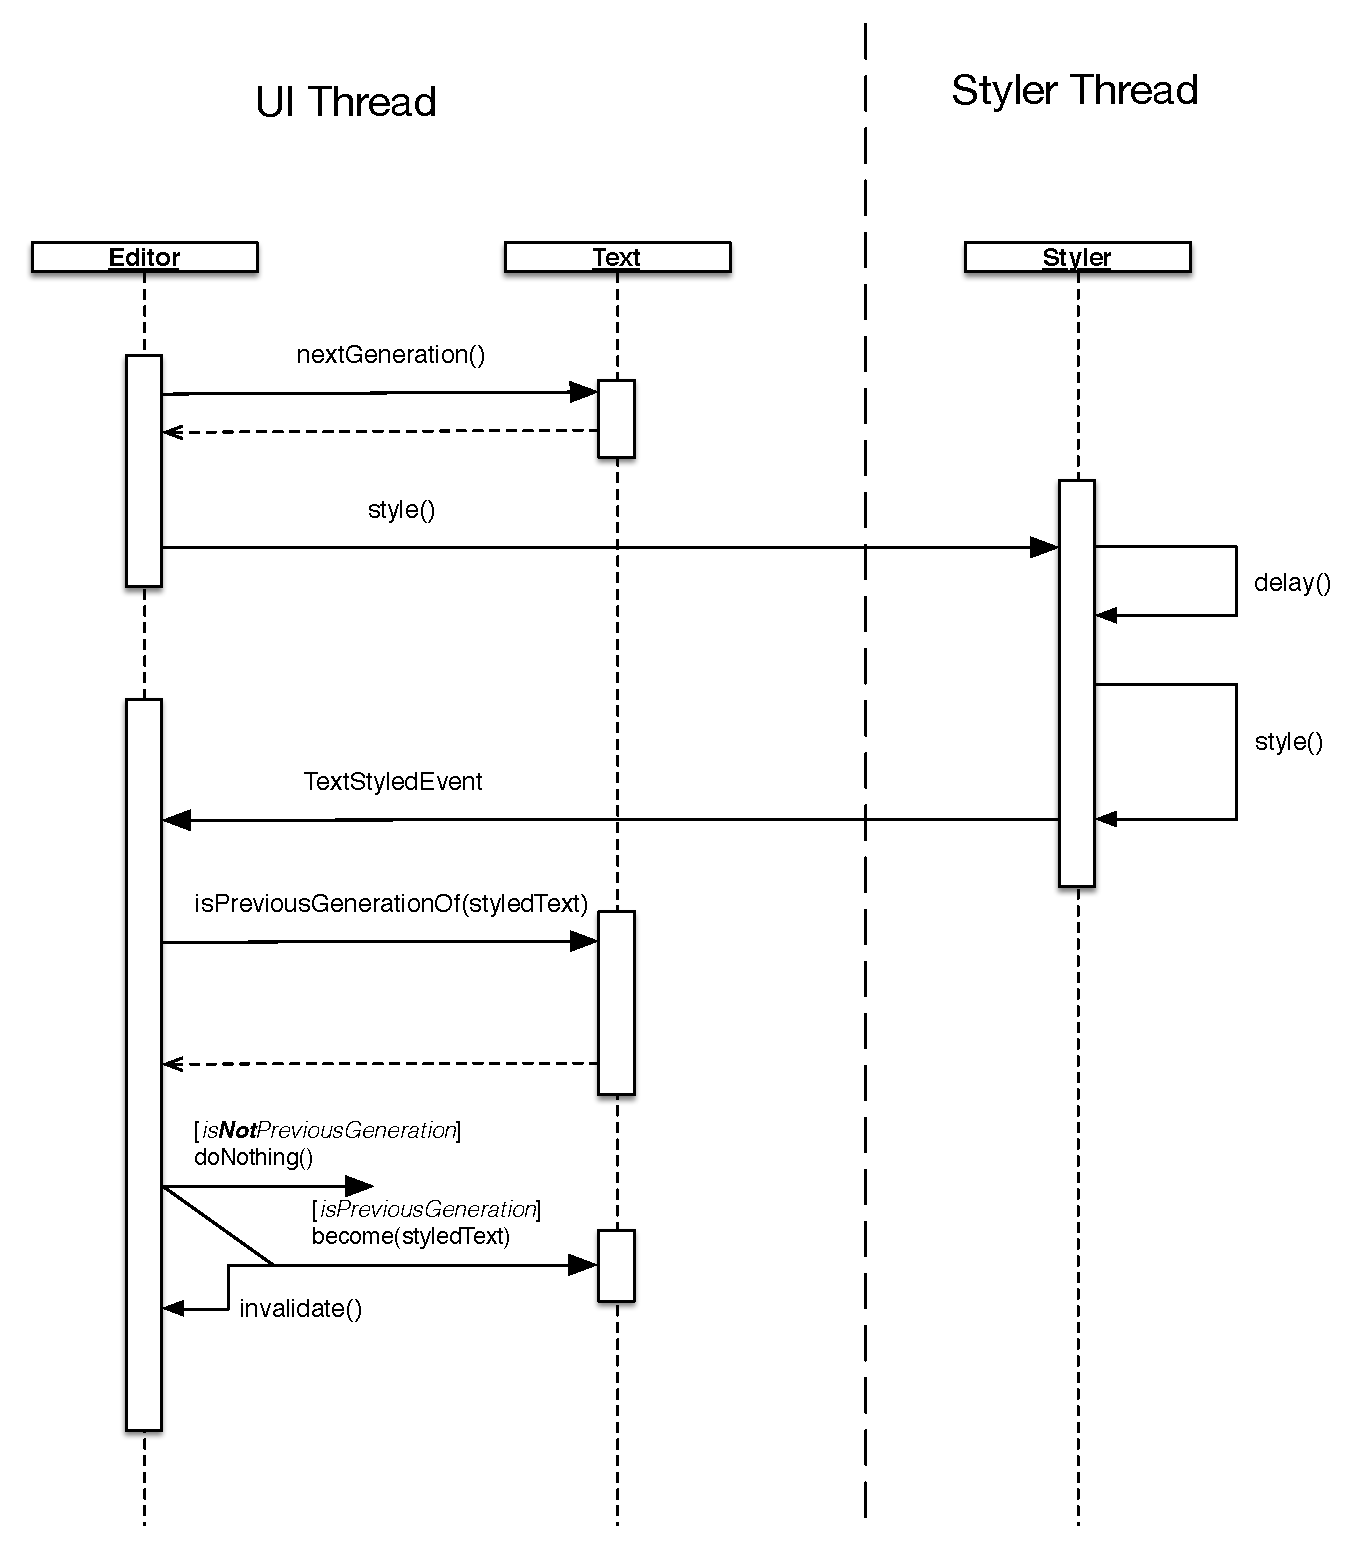
\includegraphics[width=0.78\columnwidth]{figures/editor-text-styling.pdf}
\caption{UML Sequence diagram of the styling process}
\figlabel{EditorTextStylingSequence}
\end{figure}

\newpage
As a first step the original text is asked to create a copy of itself and to mark it as a next generation: \ct{nextGeneration()}. In this case a special immutable identifier object is used to check later whether the current editor's text is still a previous generation of the one that was styled. Since \textit{Rope} is a persistent data structure it can be directly used as a generation identifier. Moreover, its immutability allows us to create new text copies without any additional overhead, because a copy simply refers to the same rope instance as a text that was copied. As soon as the editor receives a next generation back from the text it asks a styler object to perform necessary operations on that copy. On the other side, a styler responds to the \ct{style} message by terminating any existing styling process (in Pharo a green thread is called a \textit{Process}) and creating a new one that starts with a \ct{delay()} as its first operation. Delay allows styler to save computation resources by waiting until user stops typing. It improves an overall editor responsiveness as perceived by the user. Exact delay time is configurable and may vary.

As soon as text is styled a styler announces \ct{TextStyledEvent} that indicates the fact that the process is finished. That announcement is deferred on the UI thread which allows editor to handle the event in a synchronous way and perform all necessary invalidation operations without breaking editor's integrity. Then editor checks whether the original text was changed since the beginning of a styling process by making sure that a styled text is a next generation. If it is a case, the editor asks current text model to replace its content with the content of the styled one, otherwise a styled version is discarded. As a final step editor performs invalidation to update the on screen rendering to correspond a new text state.

%------------------------------------------------------------------------------------------------------------------------------------------------------------------------------
%--------------------------------------------------------- S E G M E N T S     A N D    R E N D E R I N G -----------------------------------------------------%------------------------------------------------------------------------------------------------------------------------------------------------------------------------------

\section{Segments and Rendering}
\label{SegmentsAndRenderingSection}

In order for the editor to be scalable it should be implemented in such a way that the overall performance is independent from the text size. A common technique to achieve it is to only process a part of the scene that is currently visible to the user. It means that we should not render and lay text out if it is outsize of the current viewport of the editor. Similar behaviour can be found in various graphical frameworks. A set of widgets that work only with visible elements includes for example \textit{FastTable} in Pharo, \textit{RecyclerView} in Android and others. Bloc \footnote{\url{https://github.com/pharo-graphics/Bloc}} graphical framework that is used as an underlying layer for the Moldable Editor contains such a widget, called \textit{InfiniteElement}, where \textit{infinite} stands for \textit{practically infinite} as it allows developers to create scrolling lists that are able to display large datasets. \figref{InfiniteList} shows a high level overview of the \textit{InfiniteElement's} scrolling behaviour. At any time only visible graphical elements are added to the composition tree. It allows text editor to render its content almost instantly and makes it possible to have smooth scrolling animation. When a viewport of the text editor is resized only a fraction of the overall text has to be remeasured and layered out.

\begin{figure}[h]
\centering
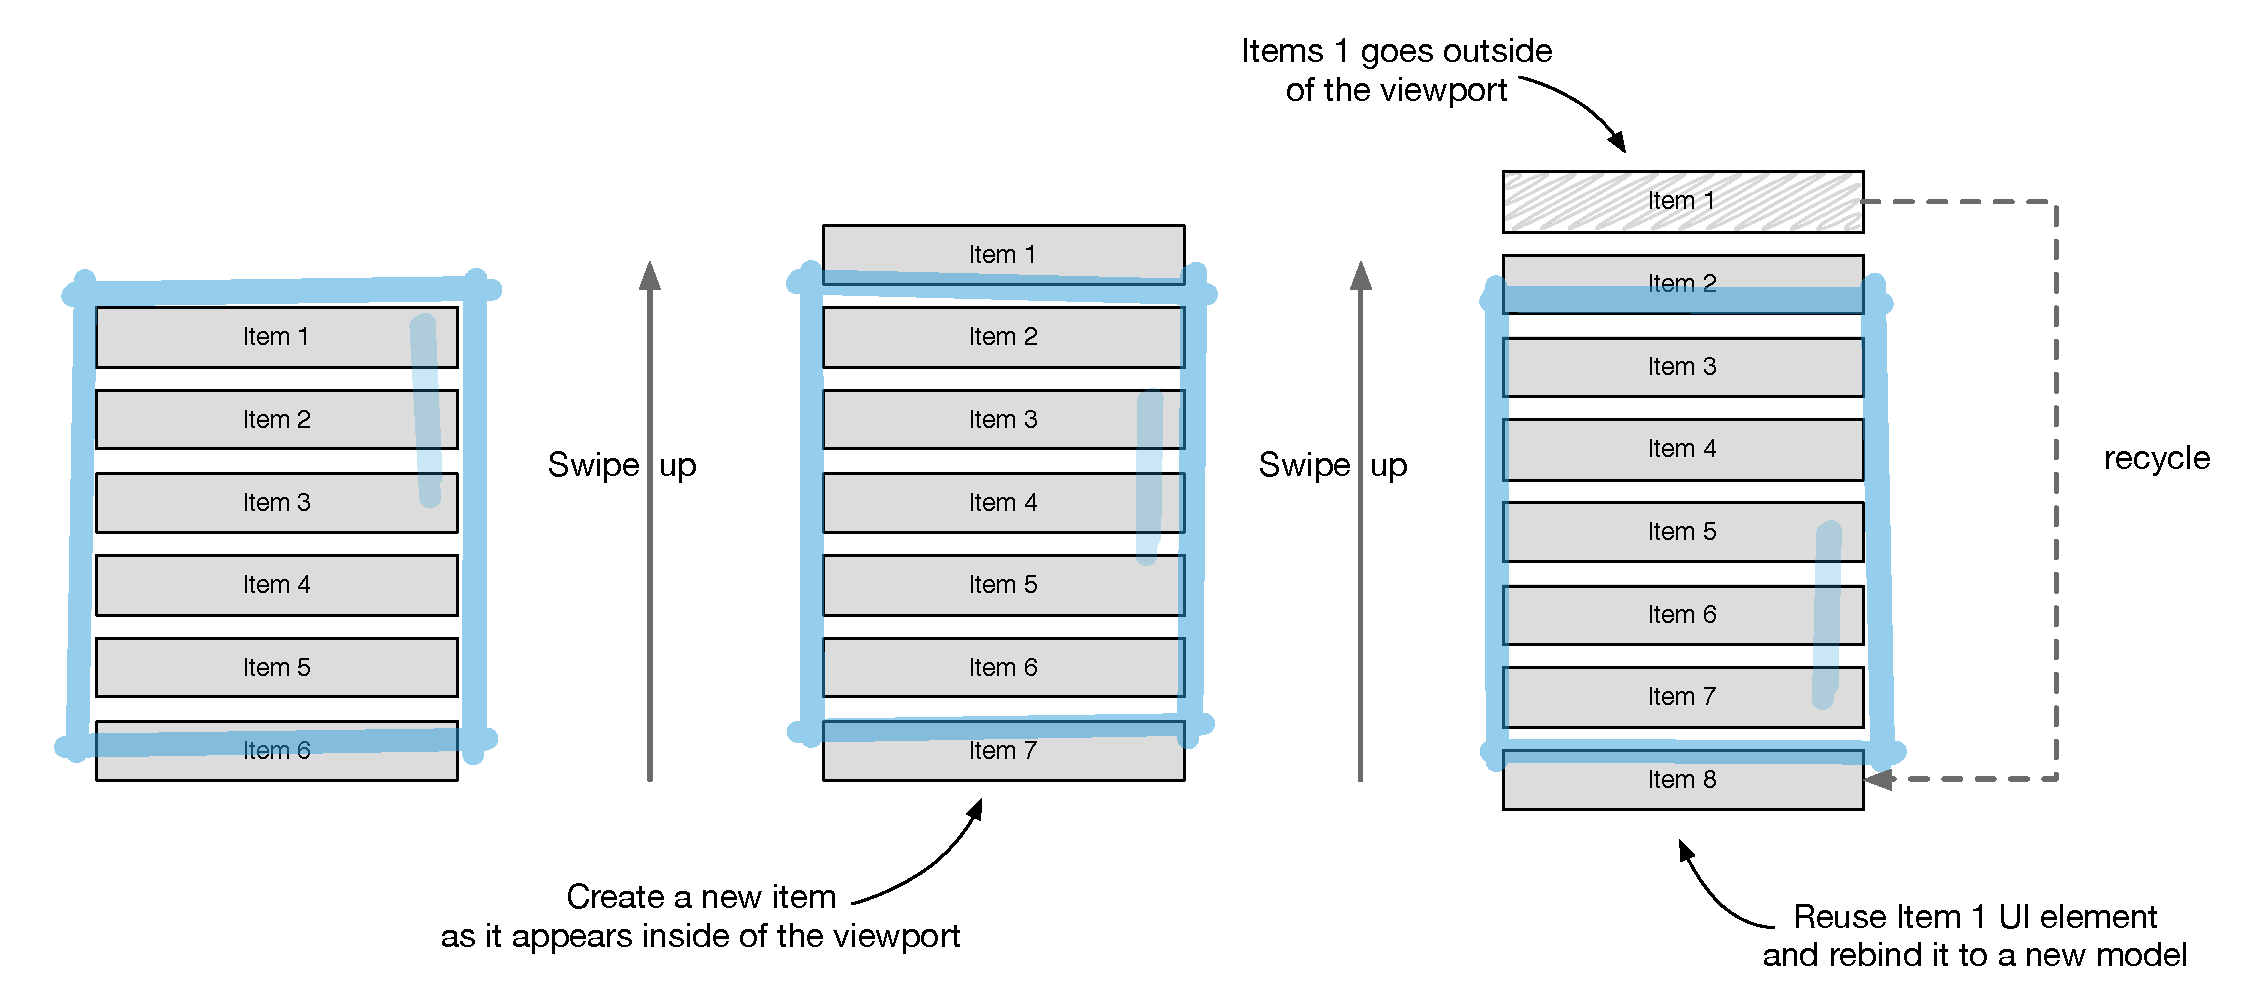
\includegraphics[width=0.75\columnwidth]{figures/infinite-list.pdf}
\caption{Scrolling items in and out of viewport using \textit{InfiniteElement}}
\figlabel{InfiniteList}
\end{figure}

However, the described approach has its own limitation. In order for the \textit{InfiniteElement} to create or reuse visual elements on demand, underlying data source has to be indexable and discrete. It means that the whole text has to be split in so called \textit{Segments}. In its current implementation, a \textit{Segment} represents a line of text, however, it can be a whole page or a collection of paragraphs. Nevertheless, if a text file is large (Gigabytes of data), reading it and splitting into segments becomes slow and inefficient. To solve this problem the editor pre-loads only a portion of the text and splits it into segments. \figref{TextModelSegments} shows how text segments are mapped on a pre-loaded portion of text and how that portion is related to the original text.

\begin{figure}[h]
\centering
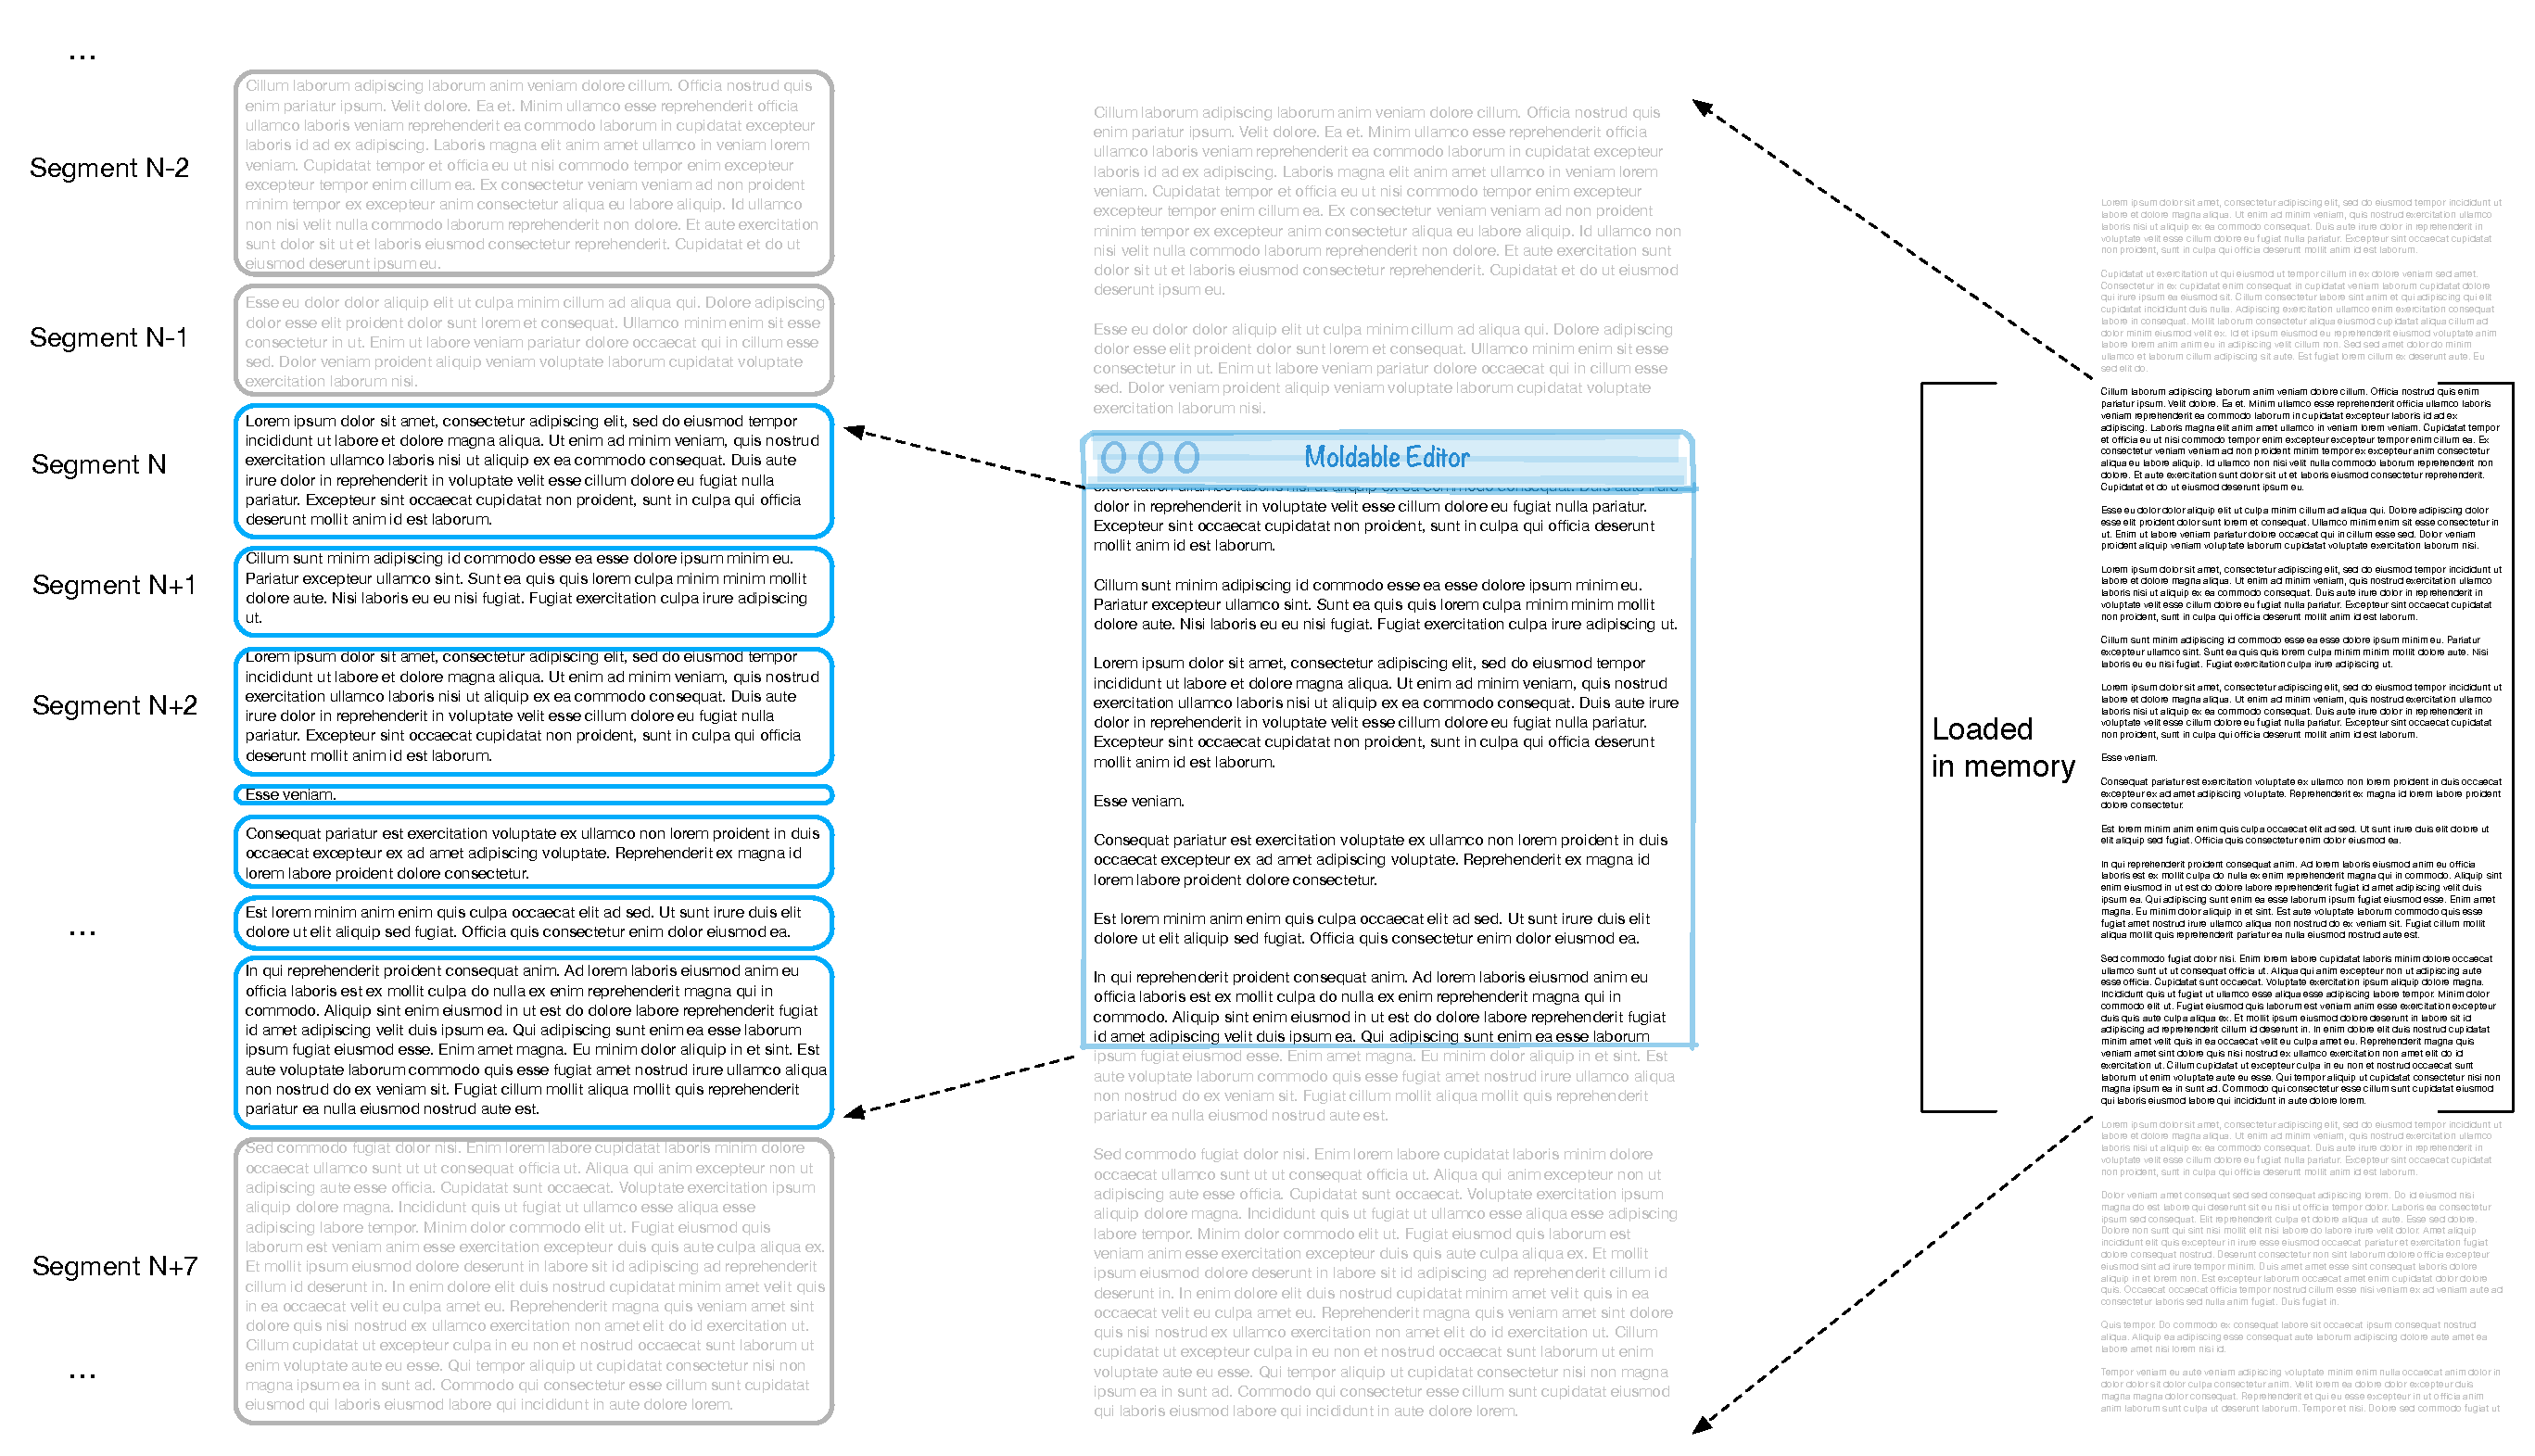
\includegraphics[width=0.85\columnwidth]{figures/text-model-segments.pdf}
\caption{Segments}
\figlabel{TextModelSegments}
\end{figure}

\newpage

Once segments are constructed, the editor creates visual elements to represent those segments. \figref{RenderingElementsMapping} shows how an editor element, opened on a two-line text, is composed. Every line is encapsulated into a segment and is rendered as \ct{TextEditorSegment.} Each segment is then split into pieces, in our case words. Finally, every word is rendered as \ct{RenderingElementsMapping.} A cursor is also a visual element and is contained by a word element which happens to have a focus. 

\begin{figure}[t]
\centering
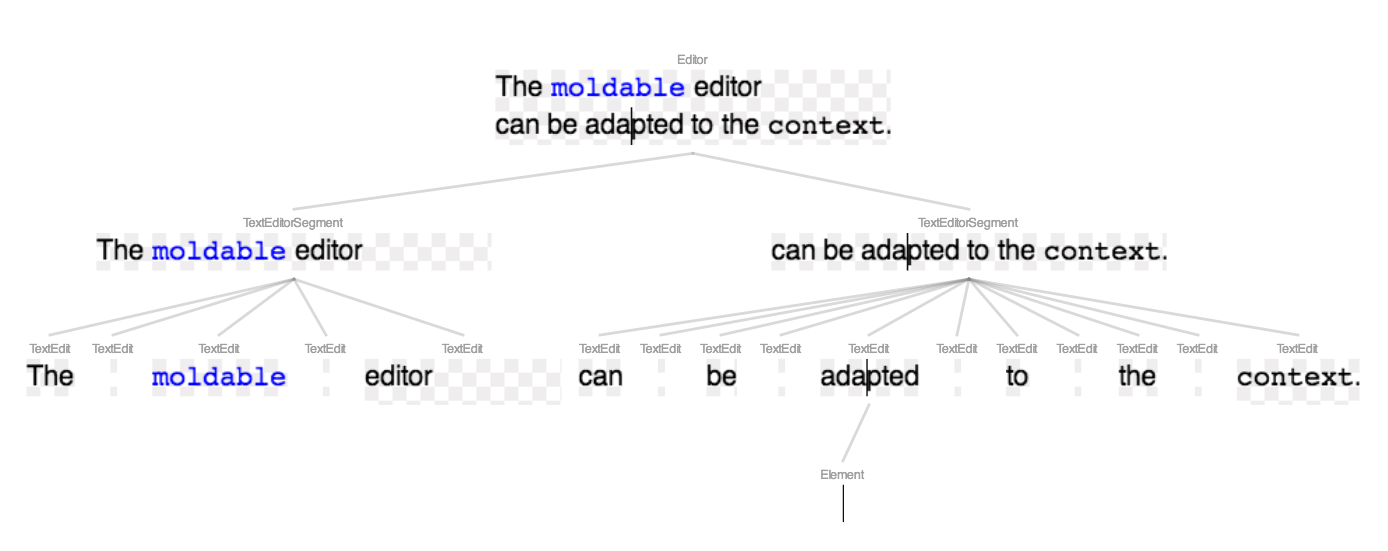
\includegraphics[width=1.0\columnwidth]{images/rendering-elements-mapping.png}
\caption{A structure of the graphical composition tree}
\figlabel{RenderingElementsMapping}
\end{figure}

%===================================================================================================
%===================================================================================================
%========================================= A P P L I C A T I O N S ========================================
%===================================================================================================
%===================================================================================================
\chapter {The Validation}


%------------------------------------------------------------------------------------------------------------------------------------------------------------------------------
%--------------------------------------------------------------------------- O V E R V I E W ---------------------------------------------------------------------------%------------------------------------------------------------------------------------------------------------------------------------------------------------------------------

\section{Overview}

\subsection*{Scalability}

The moldable editor is both flexible and scalable. For example, the following piece is a sizeable 100MB of text, and yet it opens smoothly (\figref{MoldableEditor100MB}).

\begin{figure}[h]
\centering
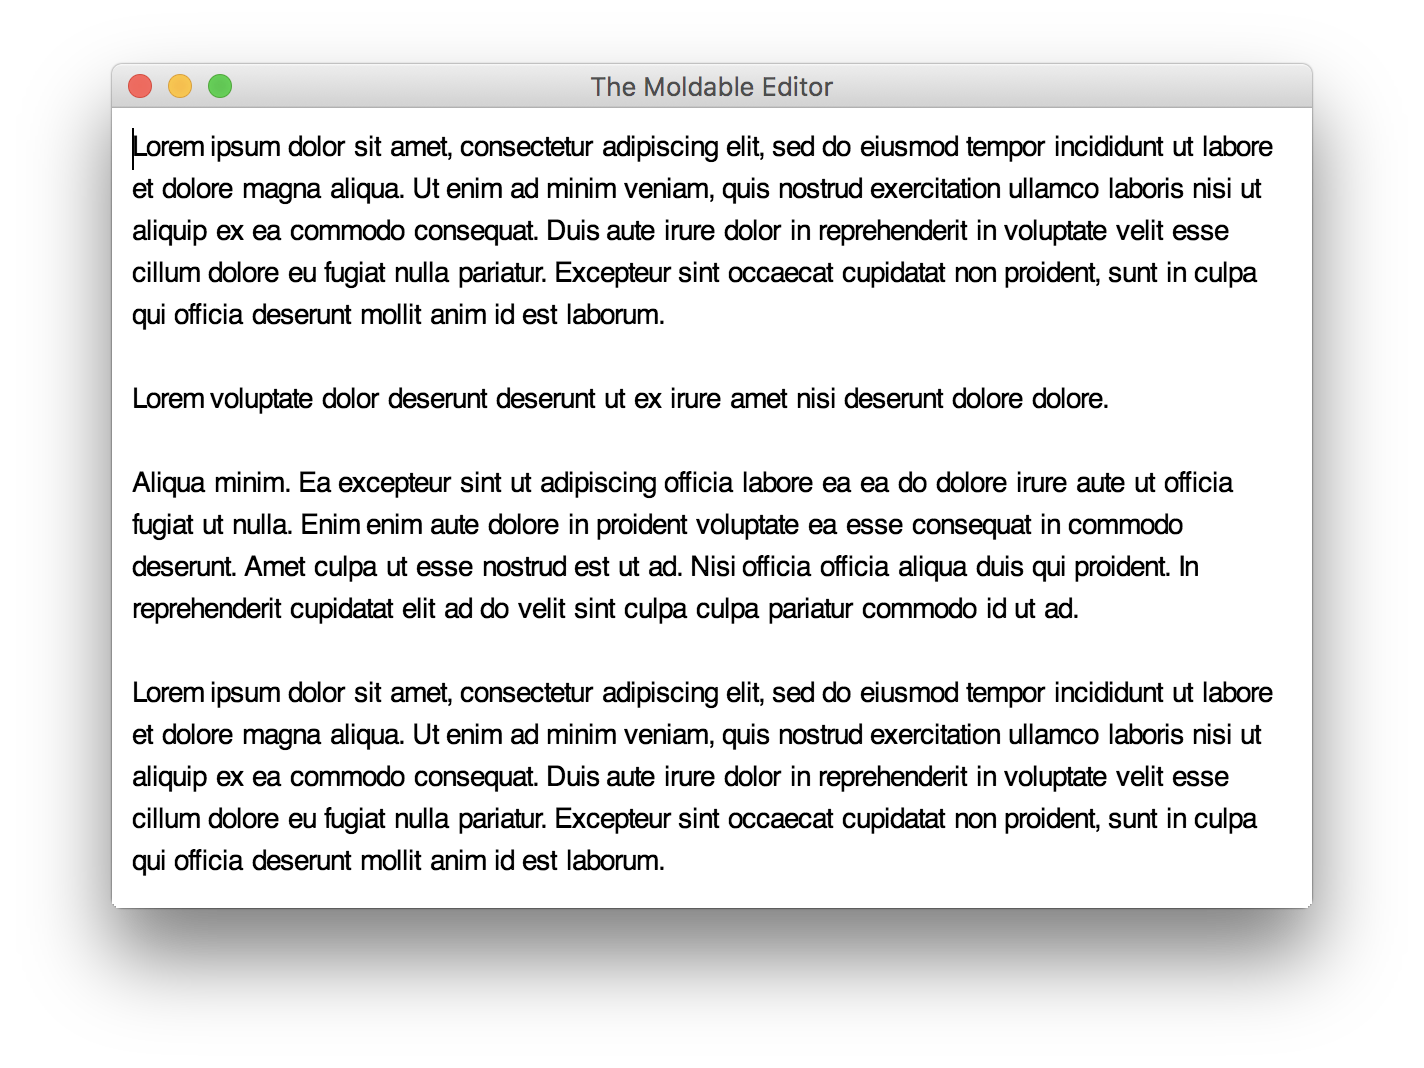
\includegraphics[width=0.65\columnwidth]{images/moldable-editor-scalable.png}
\caption{The Moldable Editor opened on a 100MB text}
\figlabel{MoldableEditor100MB}
\end{figure}

\newpage
\subsection*{Syntax highlighting and adornments}
\label{SyntaxHighlightingAndAdornments}

An obvious application for the text editor is a code editor with syntax highlighting. Like in any other text editor that supports syntax highlighting, the syntax highlighter works in a separate process and changes the existing text. Typically, the syntax highlighting affects text attributes such as color or font weight. However, the moldable editor brings this concept further and allows us to add arbitrary visual elements to a text scene.

For example, in the snippet below (\figref{EditorOnExampleCollapsed}), we see the code associated with the example that produces the editor element with syntax highlighting. In addition to the typical Pharo syntax highlighting, we can also notice small triangles inserted in the code. These triangles denote a dependency to another example method, and clicking on one expands the code in place showing another editor (\figref{EditorOnExampleExpanded}).

\begin{figure}[h]
\centering
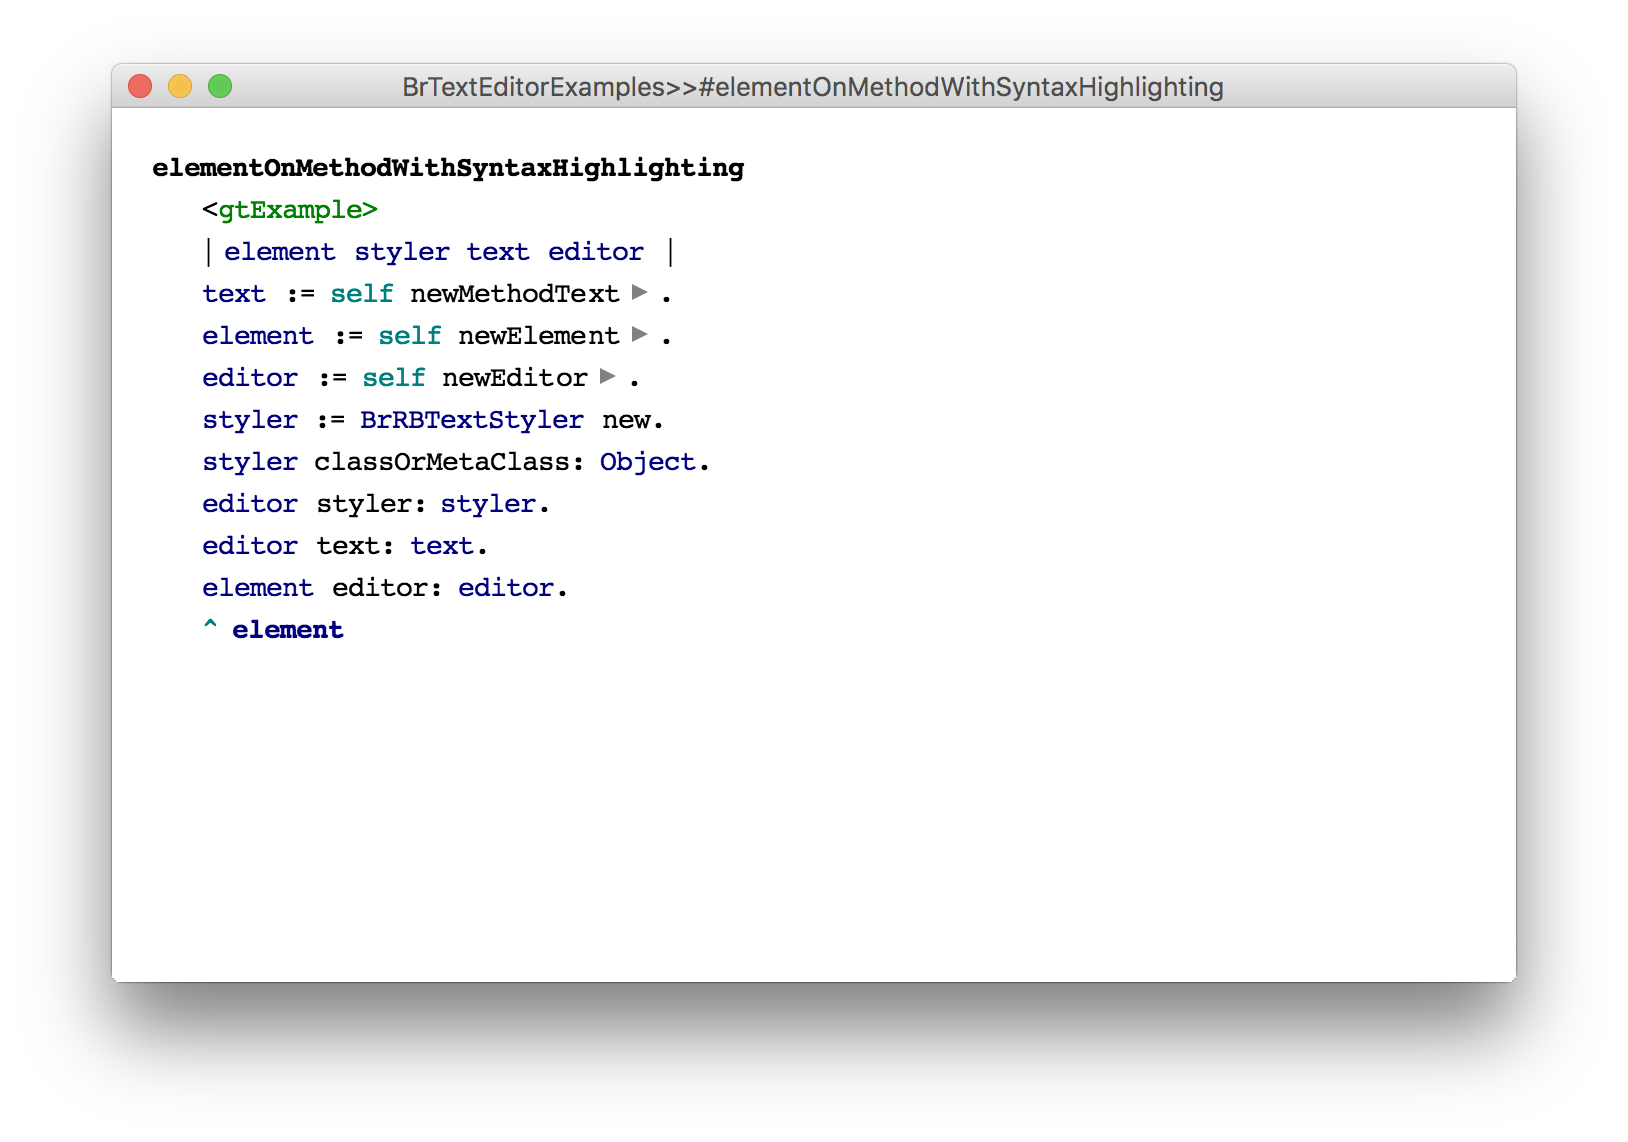
\includegraphics[width=0.9\columnwidth]{images/editor-example-collapsed.png}
\caption{The editor with syntax highlighting}
\figlabel{EditorOnExampleCollapsed}
\end{figure}

\begin{figure}[h]
\centering
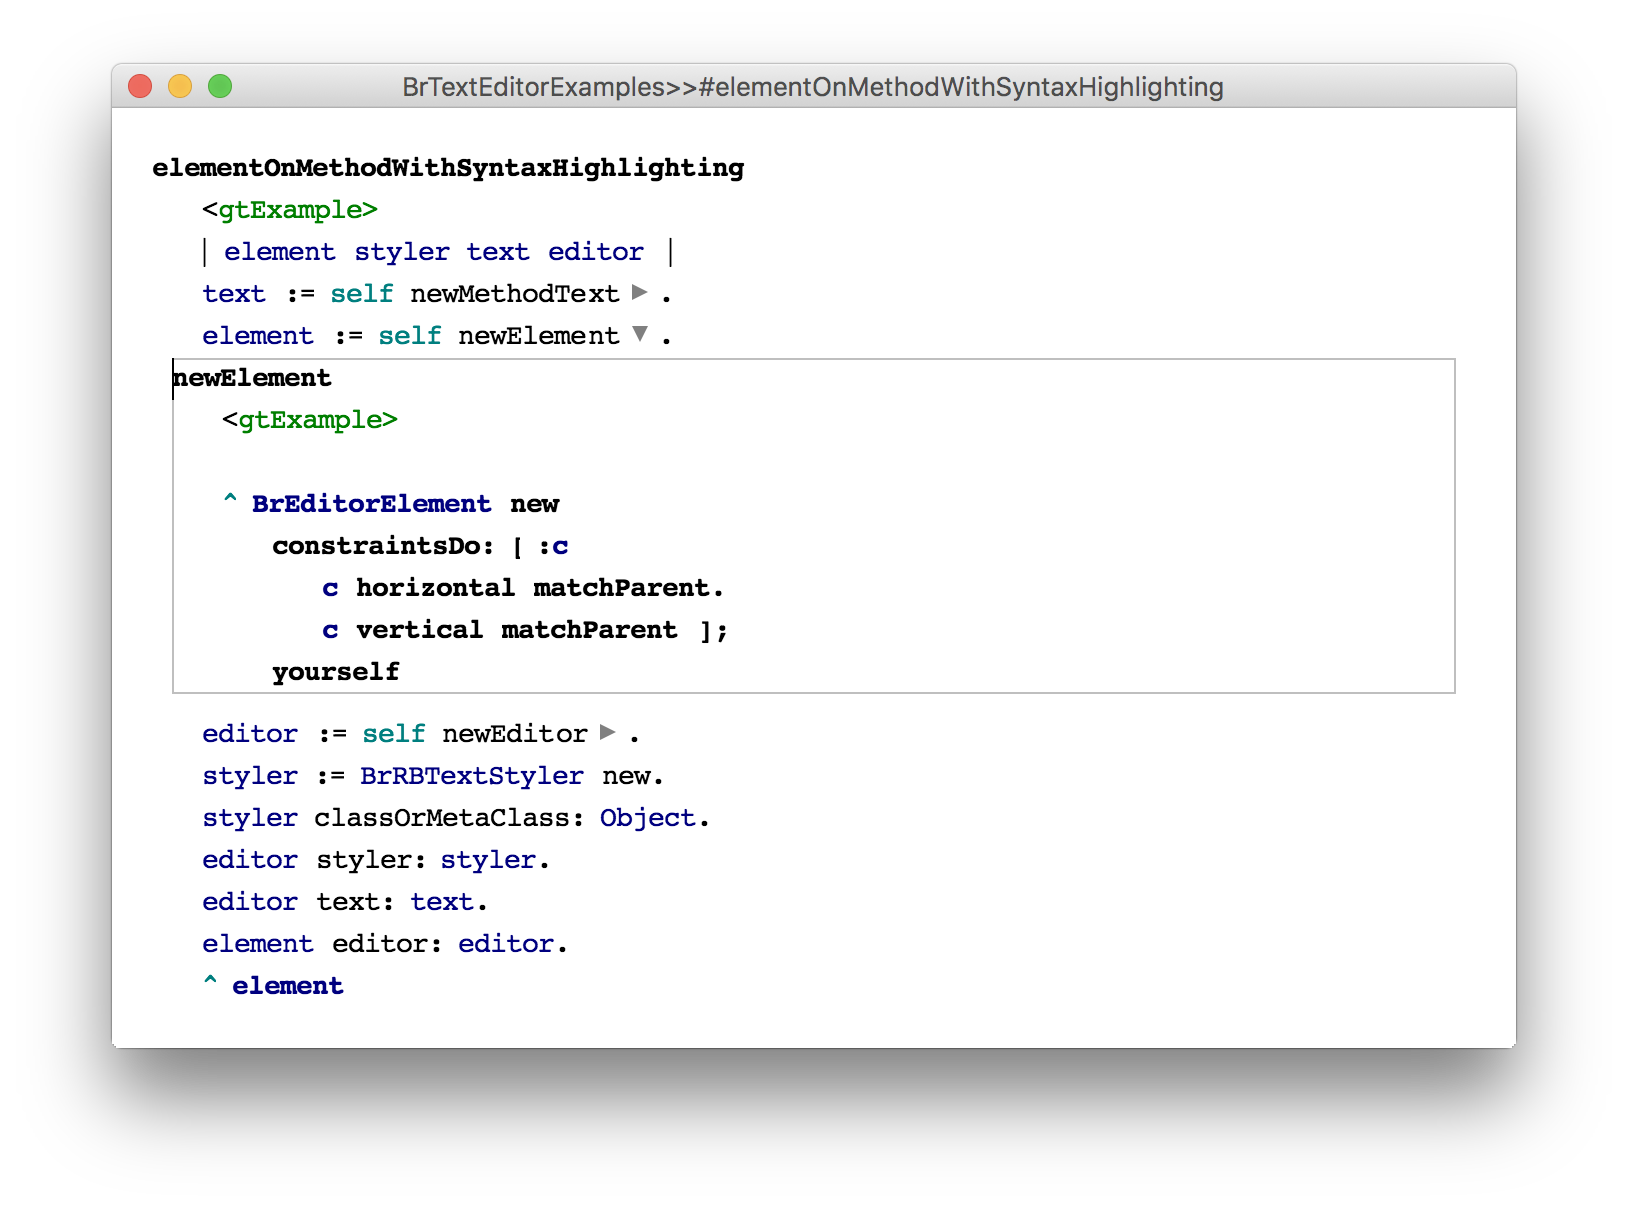
\includegraphics[width=0.85\columnwidth]{images/editor-example-expanded.png}
\caption{The editor with expanded example}
\figlabel{EditorOnExampleExpanded}
\end{figure}

This functionality is obtained through a dedicated syntax highlighter that extends the default Pharo highlighting with an extra logic that adds the triangles as adornments. Clicking on such an adornment adds another adornment with another editor element. Interestingly, this all happens live, which means that if you change the code from the root editor element to no longer refer to an example, the corresponding triangle and embedded editor elements will disappear. 

\newpage
The example above also reveals the way to initialise an editor element.


%------------------------------------------------------------------------------------------------------------------------------------------------------------------------------
%--------------------------------------------------------------------------- T R A N S C R I P T -----------------------------------------------------------------------%------------------------------------------------------------------------------------------------------------------------------------------------------------------------------
\section{Transcript}

Due to its rich abilities, the moldable editor has the potential of changing all tools that rely on textual representations. One such a tool is the Transcript.

In a context Pharo the \textit{Transcript} is a tool that allows users to log stream messages. Additionally, Pharo provides a user interface to show those messages. It means that when it comes to logging tools we should distinguish an API used to output to a stream and a user interface, which is one of the multiple ways to display  the output. Existing \textit{Transcript} in Pharo has an ability to display logged messages in a simple text editor or to write them into a file.

\begin{figure*}[t]
\centering
\subfloat[]{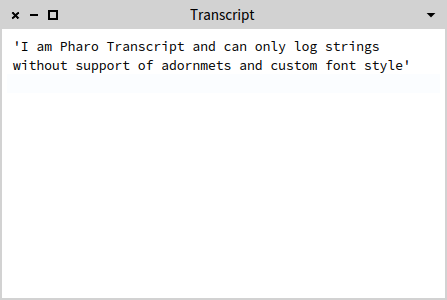
\includegraphics[width=0.32\textwidth]{images/pharo-transcript.png}\figlabel{PharoTranscript}}\hspace{0.1cm}
\subfloat[]{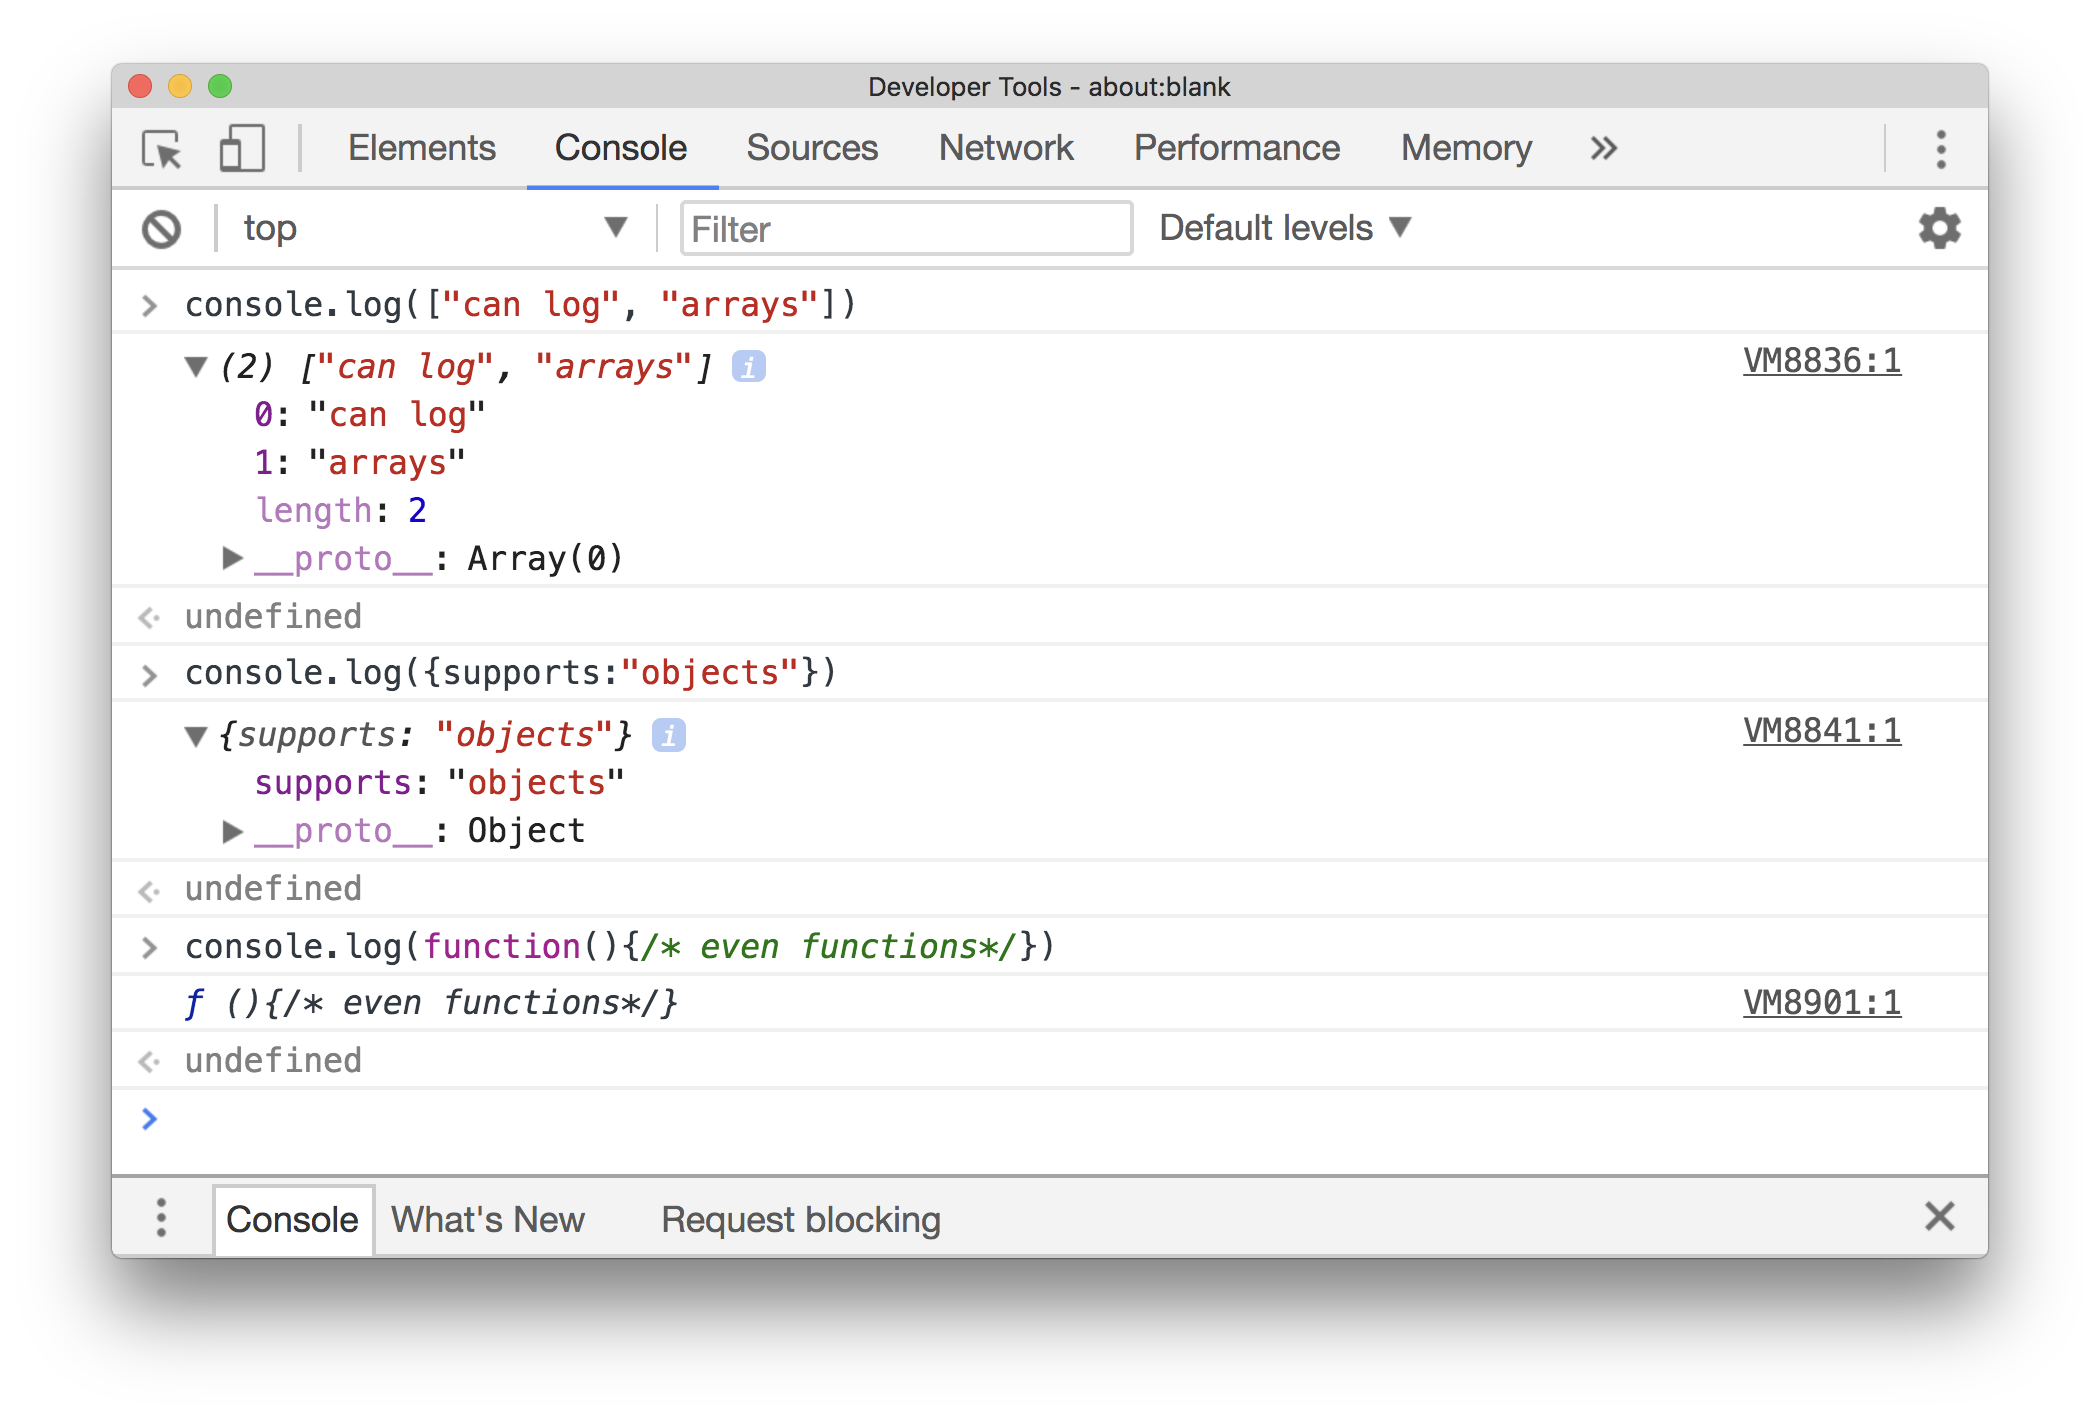
\includegraphics[width=0.32\textwidth]{images/chrome-console.png}\figlabel{ChromeConsole}}\hspace{0.1cm}
\subfloat[]{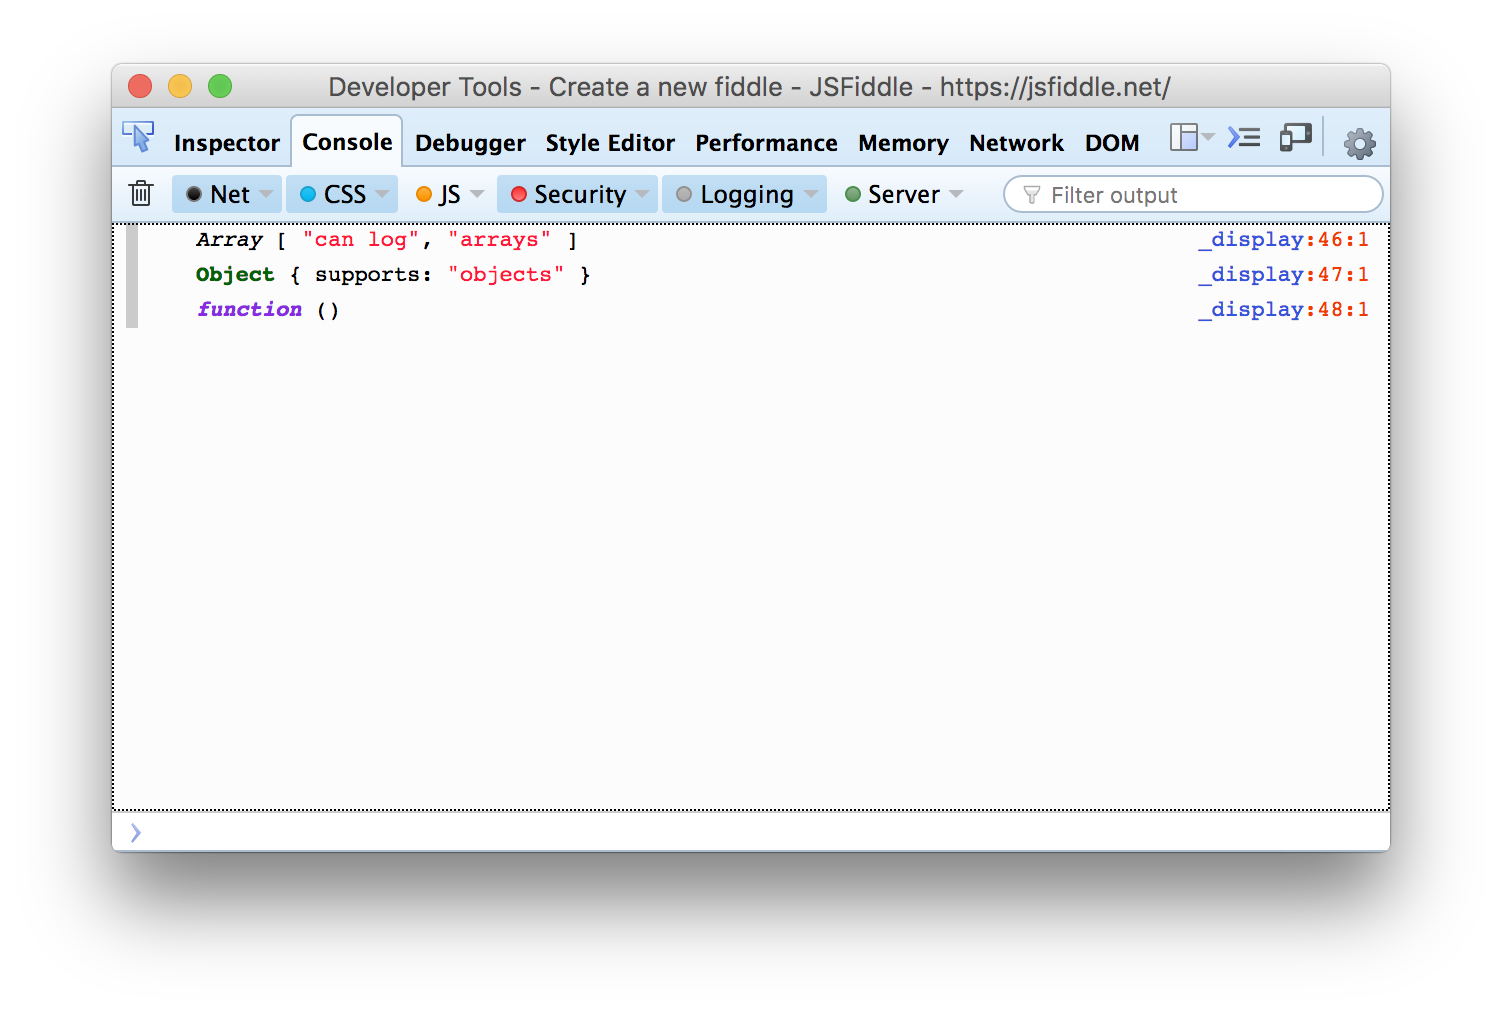
\includegraphics[width=0.32\textwidth]{images/firefox-web-console.png}\figlabel{FirefoxWebConsole}}

\caption{Examples of a transcript or console tools: \emph{a)} the standard Pharo Transcript; \emph{b)} Chrome Console; \emph{c)} Firefox WebConsole}  
\figlabel{TranscriptTools}
\end{figure*}

Many languages have support of the message logging and their IDEs provide dedicated tools allowing users to browse and read that log. For example in \textit{JavaScript}, the \textit{Console} is an object with an API that can be used to log runtime artefacts such as strings, arrays, functions or object. By default, most modern web browsers are shipped with developer tools and one of them is an interactive console. For example Mozilla Firefox provides \textit{Web Console} \footnote{\url{https://developer.mozilla.org/en-US/docs/Tools/Web_Console}} which is different from Google Chrome's \textit{Console} \footnote{\url{https://developers.google.com/web/tools/chrome-devtools/console/}} while providing very similar functionality.

The goal of GT Transcript is to offer a rich and interactive interface for displaying live information coming from a system.  

\subsection*{The API}

The API is backward compatible with the existing transcript. To enable the new features, we introduced a builder. For example, \ct{transcript nextPutAll: 'something'} becomes \ct{transcript next putAll: 'something'}. Between \textit{next} and \textit{putAll:}, we can add multiple attributes to the text output.

\begin{figure}[t]
\centering
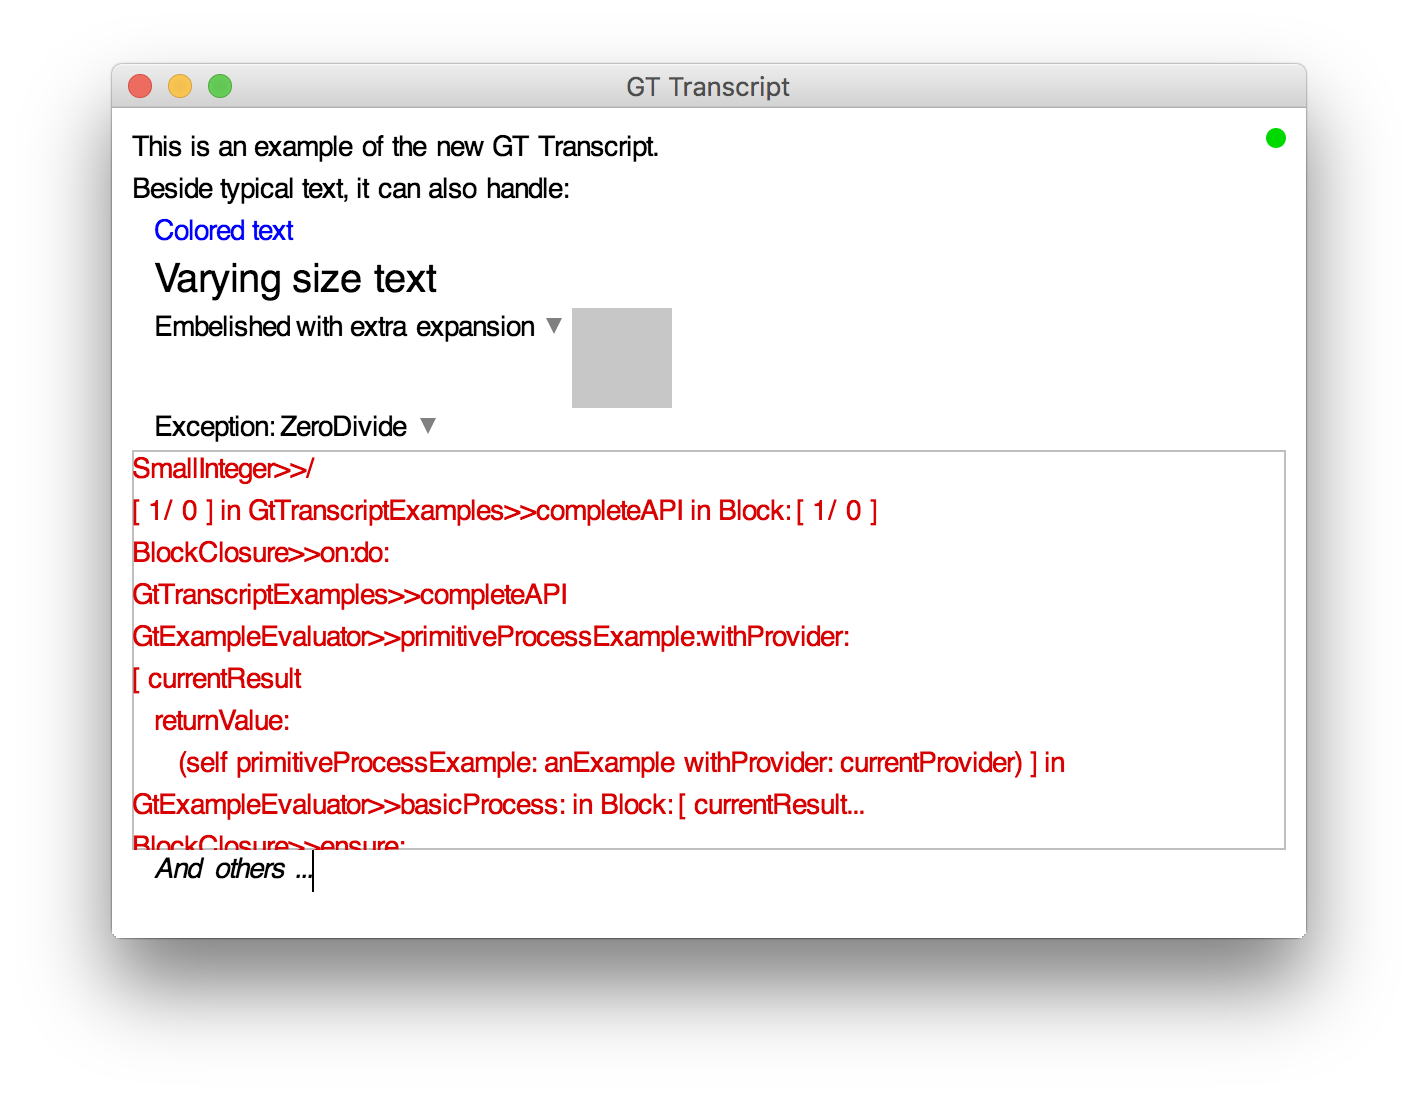
\includegraphics[width=0.65\columnwidth]{images/gt-transcript-complete-api.png}
\caption{Visual output of \lstref{GtTranscriptCompleteApiCode}}
\figlabel{GtTranscriptCompleteApi}
\end{figure}

\begin{minipage}[t]{0.95\textwidth}

The following example shows the complete API:

\begin{lstlisting}[language=Smalltalk, caption={The complete API of the GT-Transcript},captionpos=b, label={lst:GtTranscriptCompleteApiCode}]
| transcript |
transcript := GtTranscript new.
transcript 
	nextPutAll: 'This is an example of';
	space;
	nextPutAll: 'the new GT Transcript';
	nextPut: '.';
	cr.
transcript next
	putAll: 'Beside typical text, it can also handle:';
	cr.
transcript next
	tab;
	color: Color blue;
	putAll: 'Coloured text';
	cr.
transcript tab.
transcript next	
	fontSize: 20;
	putAll: 'Varying size text';
	cr.
transcript next
	tab;
	expanding: [ BlElement new background: Color gray ];
	putAll: 'Embellished with extra expansion';
	cr.
[ 1/0 ] on: Error do: [ :err | 
	transcript next 
		tab;
		putAll: 'Exception: ';
		showException: err;
		cr ].
transcript next 
	tab;
	italic;
	streamAll: [ transcript next putAll: 'And others ...' ].
\end{lstlisting}

\end{minipage}

\newpage
\subsection*{Logging an animation}

When working on animations it is important to be able to debug them. Developers may find themselves in a situation where debugger is not helpful since it stops an animation process and only lets programmers to browse a frozen state. A different approach would be to observe how animation progresses over time. Traditionally, developers would insert logging statements and output changing parameters. However, textual representation may be a limited source of information. Instead, we propose to use GT Transcript, for visual logging of animation providing insight far superior to plain text.

To get an idea of how this tool can be useful, take a look at the following example on the \figref{GtTranscriptAnimation}:

\begin{figure}[h]
\centering
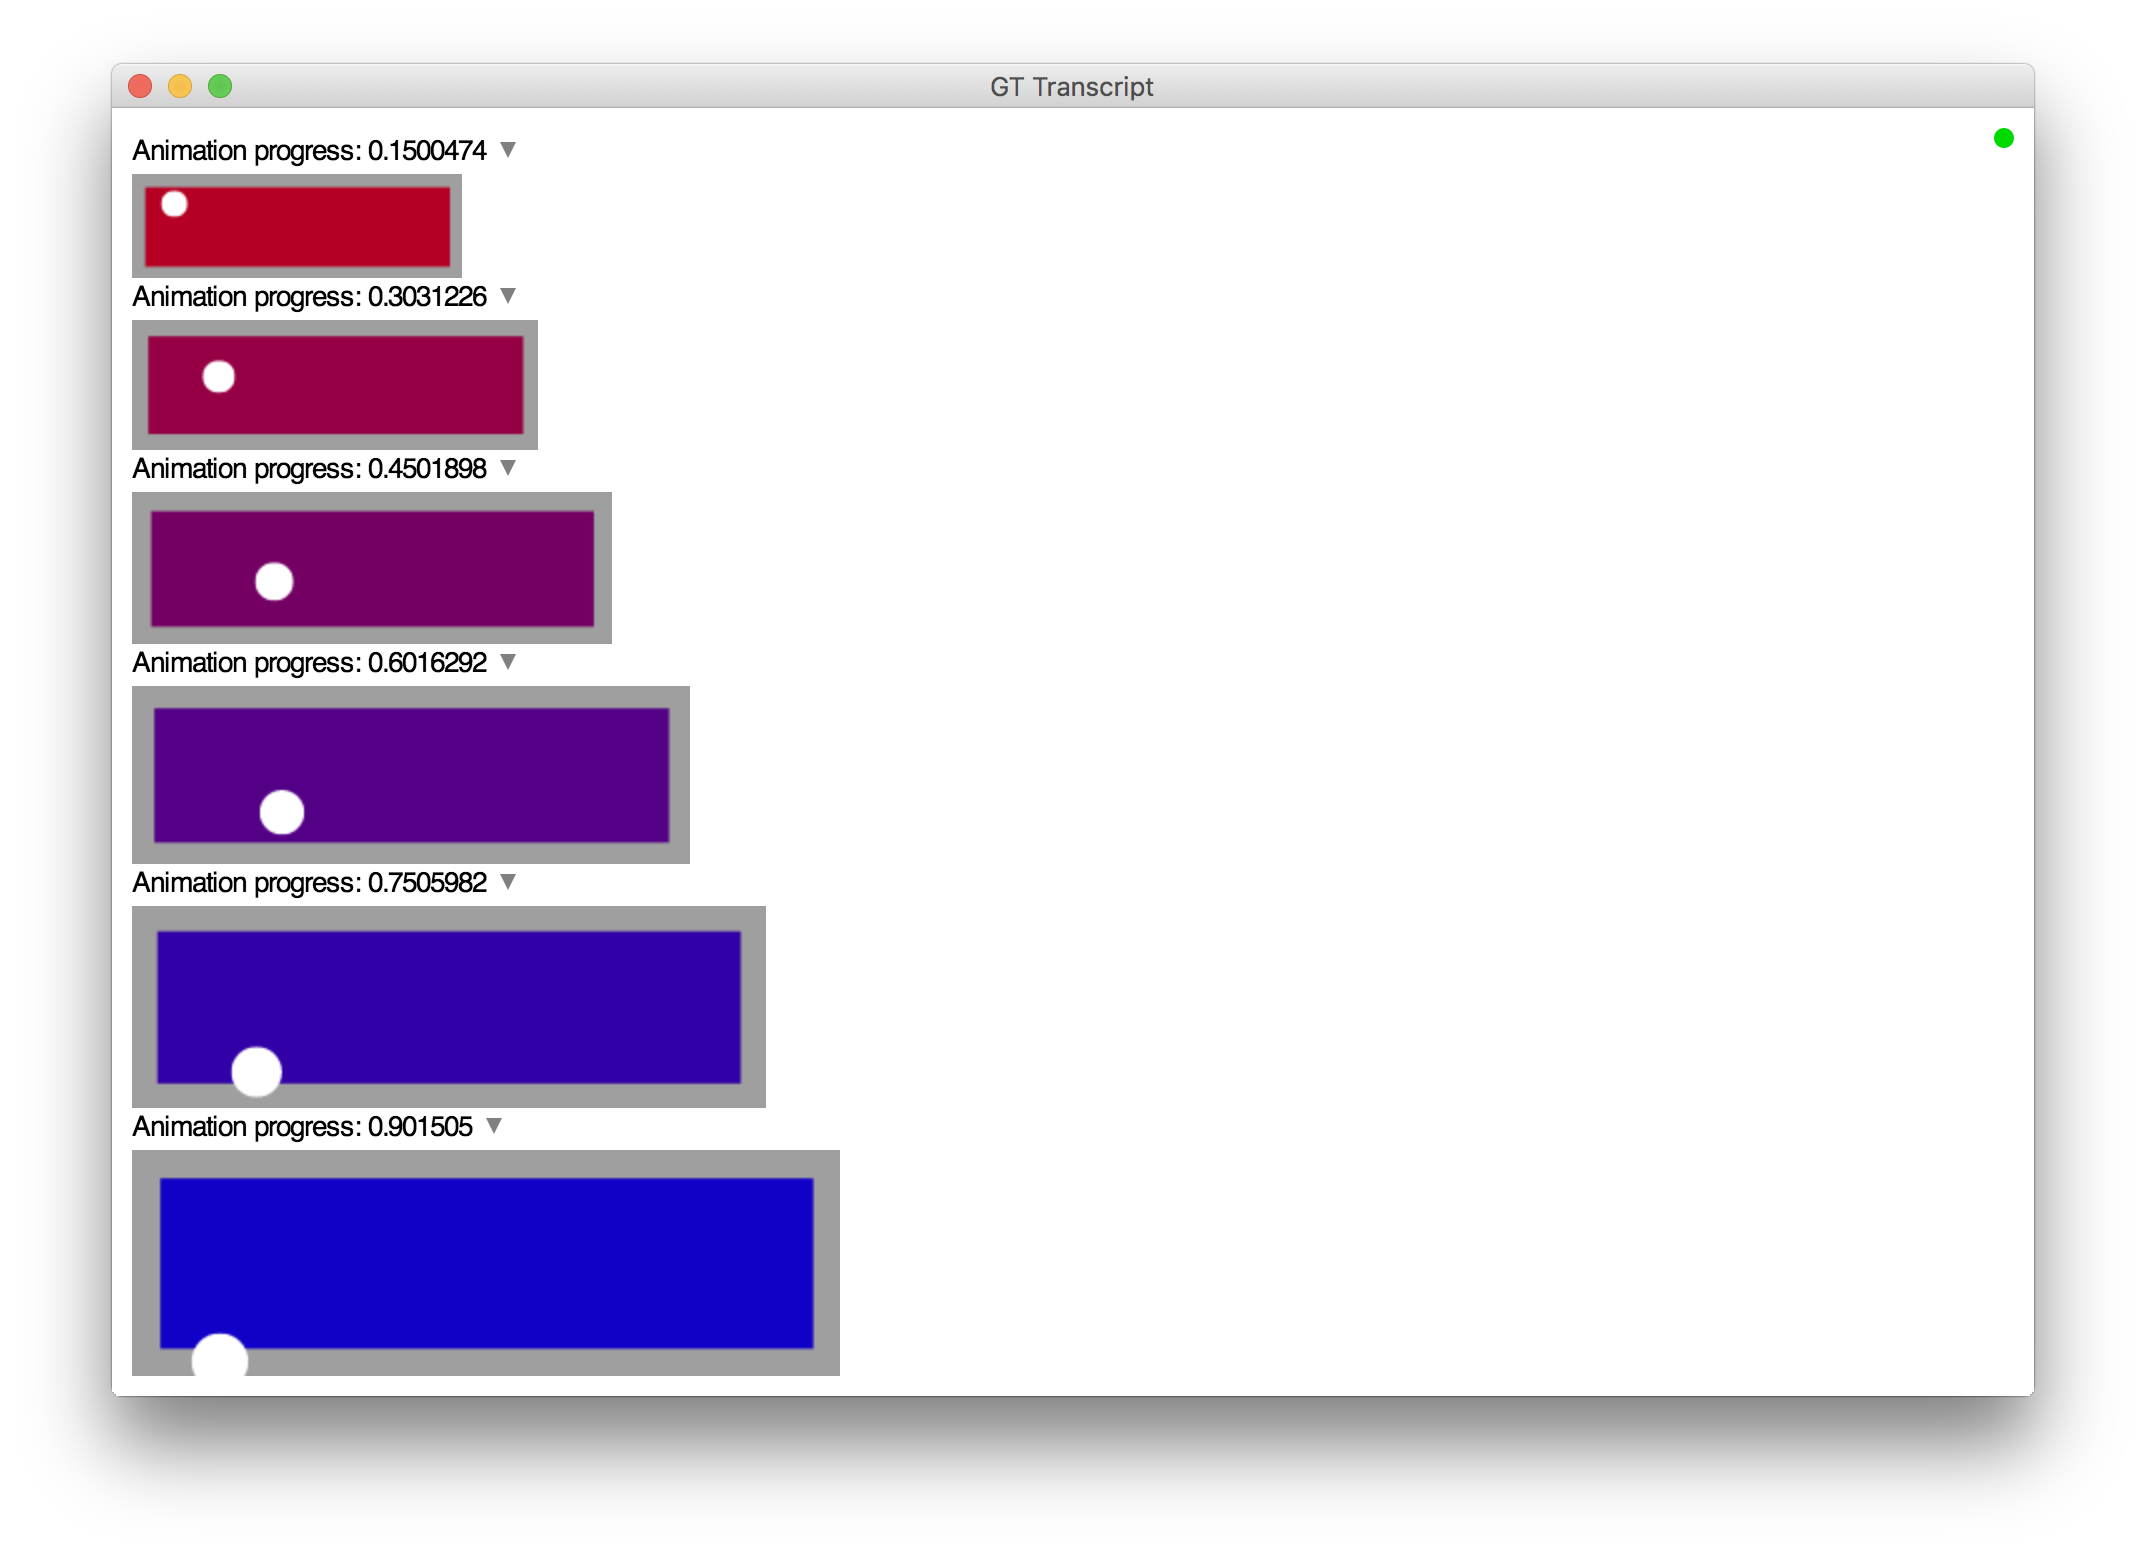
\includegraphics[width=0.8\columnwidth]{images/gt-transcript-animation.png}
\caption{Visual logging of Animation with GT Transcript}
\figlabel{GtTranscriptAnimation}
\end{figure}

There we have a rectangle element with a white circle element as its direct child. Once element is constructed we apply a composite Bloc animation that consists of scale transformation, color transition. Additionally, we apply translation animation on the circle. During the animation multiple parameters get changed which makes textual logging a tedious task. However, instead of text users could directly log visual elements, which appear as image snapshots in the Transcript.

\bigskip

To implement GT Transcript there were no changes made to the underlying editor model and all additional functionality was easily integrated which indicates editor's flexibility. In the following sections we continue to validate the Moldable Editor by putting it in more different contexts.

%------------------------------------------------------------------------------------------------------------------------------------------------------------------------------
%--------------------------------------------------------------------------- C O N N E C T O R -----------------------------------------------------------------------%------------------------------------------------------------------------------------------------------------------------------------------------------------------------------
\newpage
\section{Connector}

In Section \ref{SyntaxHighlightingAndAdornments}, we saw how example dependencies can be expanded in place by using the syntax highlighter. Connector brings this a step further and proposes a new kind of interface that allows users to expand a new editor on an example method and to automatically connect editor elements with one another.
The interface is somewhat similar to the one proposed by Code Bubbles \footnote{\url{http://cs.brown.edu/~spr/codebubbles/}}\cite{Brag10a}.

\begin{figure}[h]
\centering
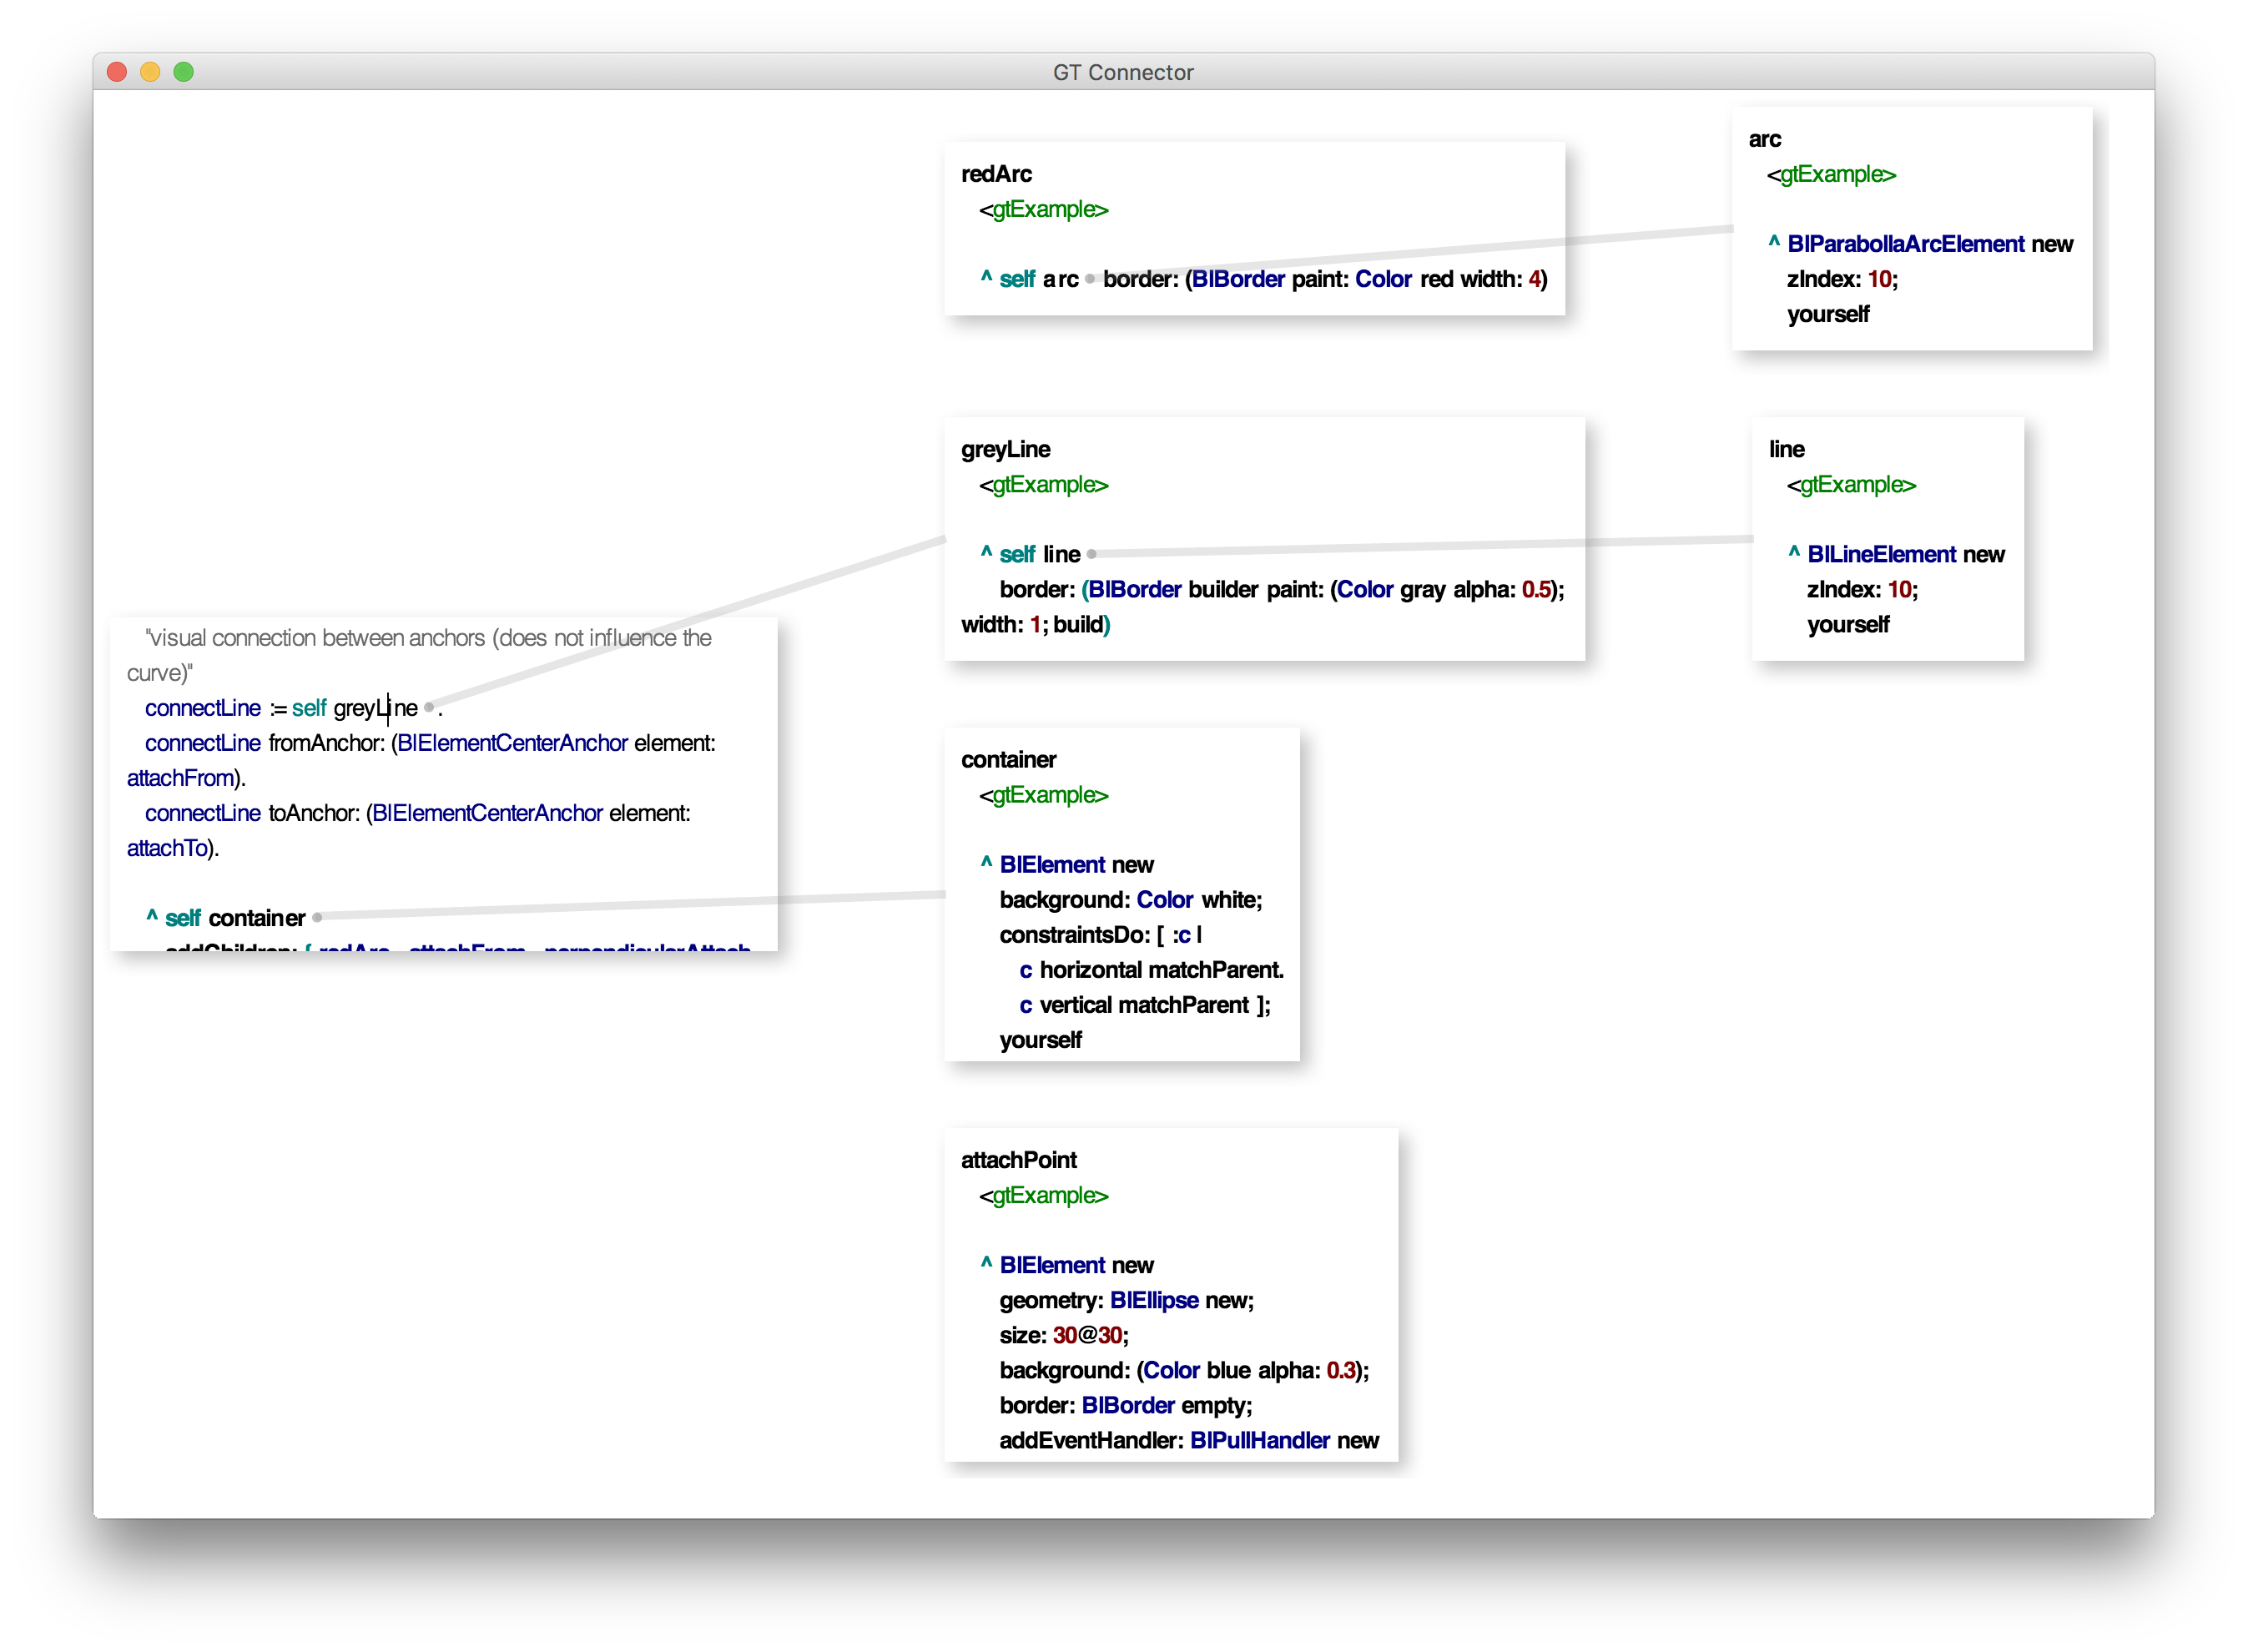
\includegraphics[width=0.85\columnwidth]{images/gt-connector.png}
\caption{GT Connector opened on an example method}
\figlabel{GtConnector}
\end{figure}

However, it has two key differences:
\begin{itemize}  
\item the lines connect an element inside the text editor to the outside world. This is possible because the text is represented as elements that are rendered in the main rendering tree provided by the underlying Bloc framework.
\item the lines are added automatically to reveal dependencies that are otherwise more difficult to spot.
\end{itemize}

%------------------------------------------------------------------------------------------------------------------------------------------------------------------------------
%-------------------------------------------------------------------------- D O C U M E N T E R ---------------------------------------------------------------------%------------------------------------------------------------------------------------------------------------------------------------------------------------------------------
\newpage
\section{Documenter}

Documentation plays an important role during development process. Developers spend a sizeable amount of time on writing it, maintaining and evolving over time. Nowadays there exist techniques and automatisation processes that allow developers to create \textit{technical documentation} out of existing source code. Examples of such tools include Javadoc\footnote{\url{https://docs.oracle.com/javase/9/javadoc/javadoc.htm}}, Doxygen\footnote{\url{http://doxygen.org/}}, Visual Expert\footnote{\url{http://www.visual-expert.com/}}, to name a few. They help programmers to keep documentation up-to-date with almost no effort (\figref{Javadoc}). However, such documentation is too technical and may not satisfy all the needs of the users. Instead of browsing auto-generated documentation users of a library or a framework could benefit more from \textit{user documentation} such as tutorials, blog posts, thematics, guides or cheatsheets. One of the key-points of user documentation is an ability to mix plain text explanations with code snippets and some sort of a preview of the result of those code snippets, sometimes in a form of screenshots. That is where a problem of user documentation comes from; tutorials must be updated due to API changes or UI improvements that may lead to visible differences between screenshots and an actual output of the code snippets if they would be executed in a real environment. Additionally, tutorials are not meant to be testable in any automatic way, for example on CI servers. As a result it increases the cost of maintaining user documentation and may even have a negative impact if new users face issues or discrepancies in their expectations based on tutorial and real results.

\begin{figure*}[h]
\centering
\subfloat[]{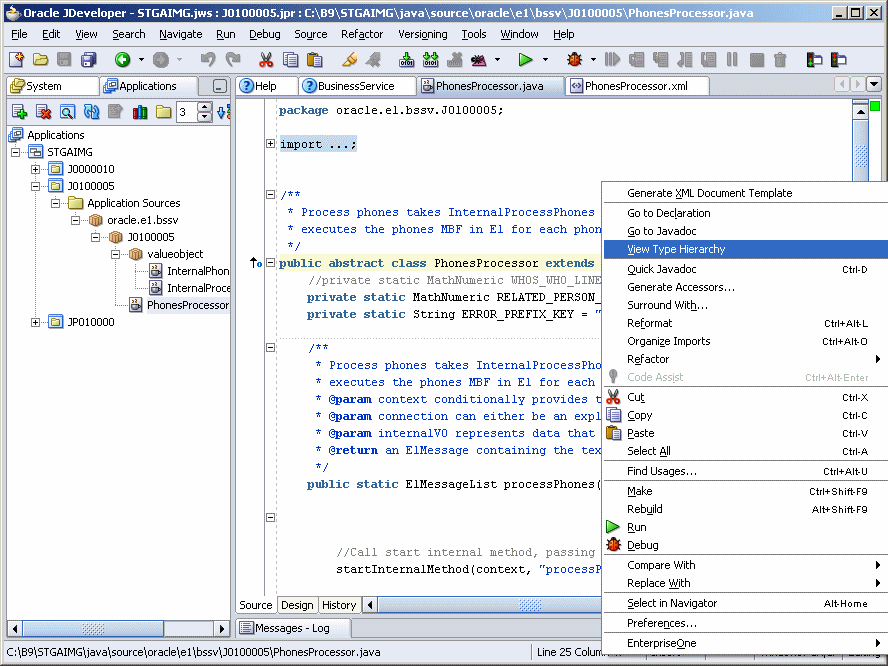
\includegraphics[width=0.48\textwidth]{images/javadoc-sourcecode.png}\figlabel{JavadocSourceCode}}\hspace{0.1cm}
\subfloat[]{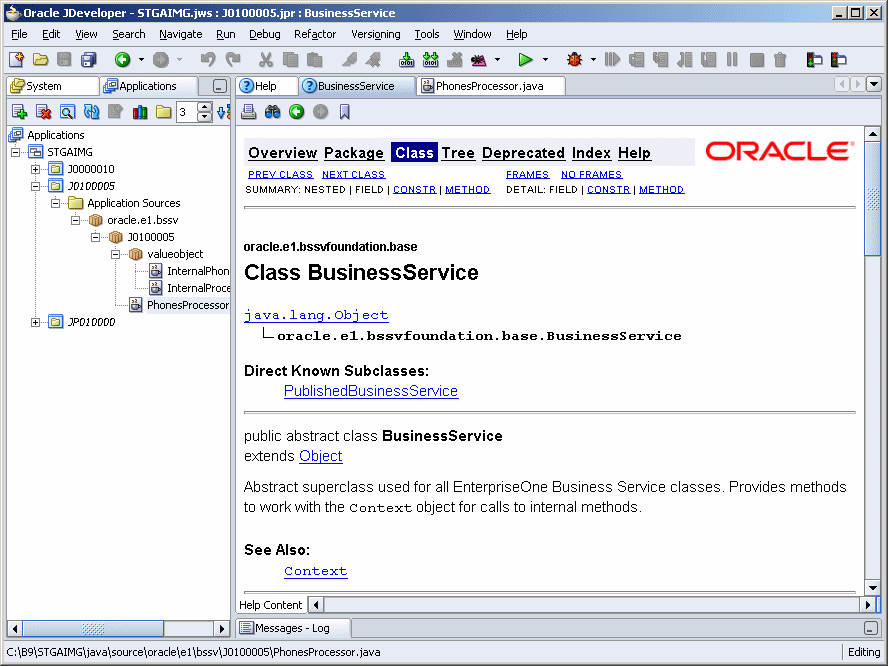
\includegraphics[width=0.48\textwidth]{images/javadoc-documentation.png}\figlabel{JavadocDocumentation}}\hspace{0.1cm}

\caption{Two sides of Javadoc: \emph{a)} source code; \emph{b)} generated documentation}  
\figlabel{Javadoc}
\end{figure*}

\newpage

The goal of the Documenter is to reduce a cost of maintaining user documentation and make it easier for developers to write it.

As a way to achieve it, the Documenter offers live rendering of Pillar\footnote{\url{https://ci.inria.fr/pharo-contribution/job/EnterprisePharoBook/lastSuccessfulBuild/artifact/book-result/PillarChap/Pillar.html}} documents. For example, as shown on \figref{GtDocumenterMondrianExamplePictures} Documenter can embed pictures right in place.

\begin{figure}[h]
\centering
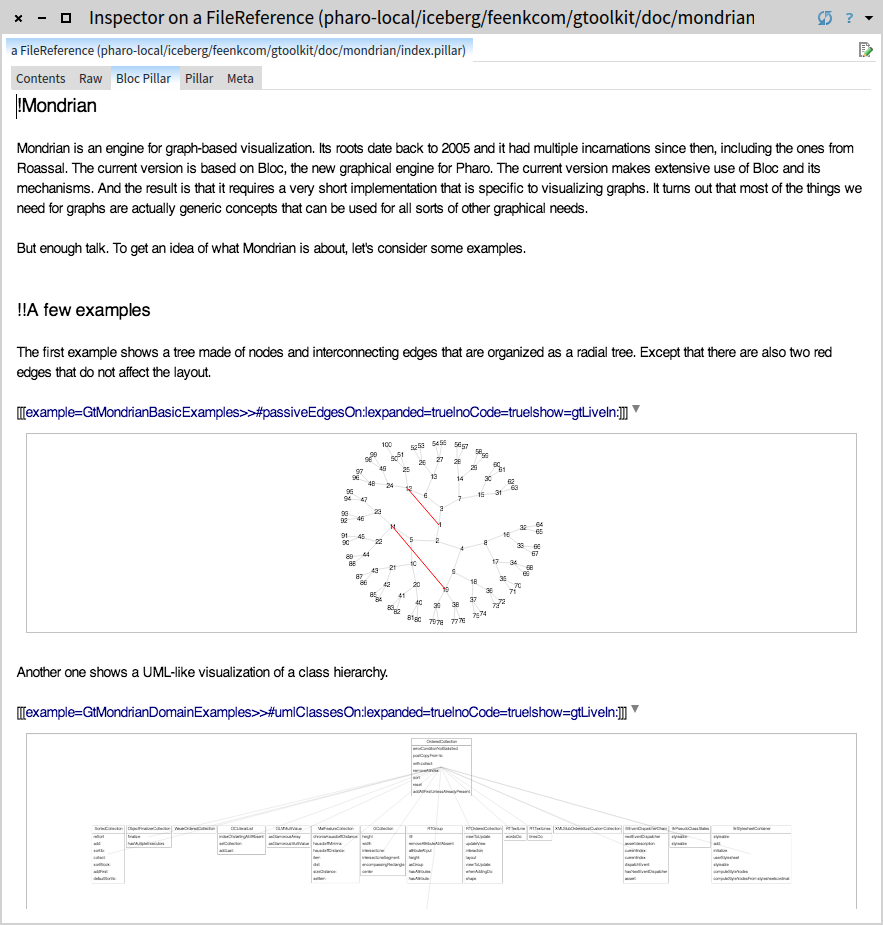
\includegraphics[width=0.95\columnwidth]{images/documenter-mondrian-example-pictures.png}
\caption[The LOF caption]{Documenter opened on a Mondrian\footnotemark  documentation file}
\figlabel{GtDocumenterMondrianExamplePictures}
\end{figure}
\footnotetext{\url{https://github.com/feenkcom/gtoolkit-visualizer}}

\newpage
And it can even embed live code that can be previewed in place:

\begin{figure}[h]
\centering
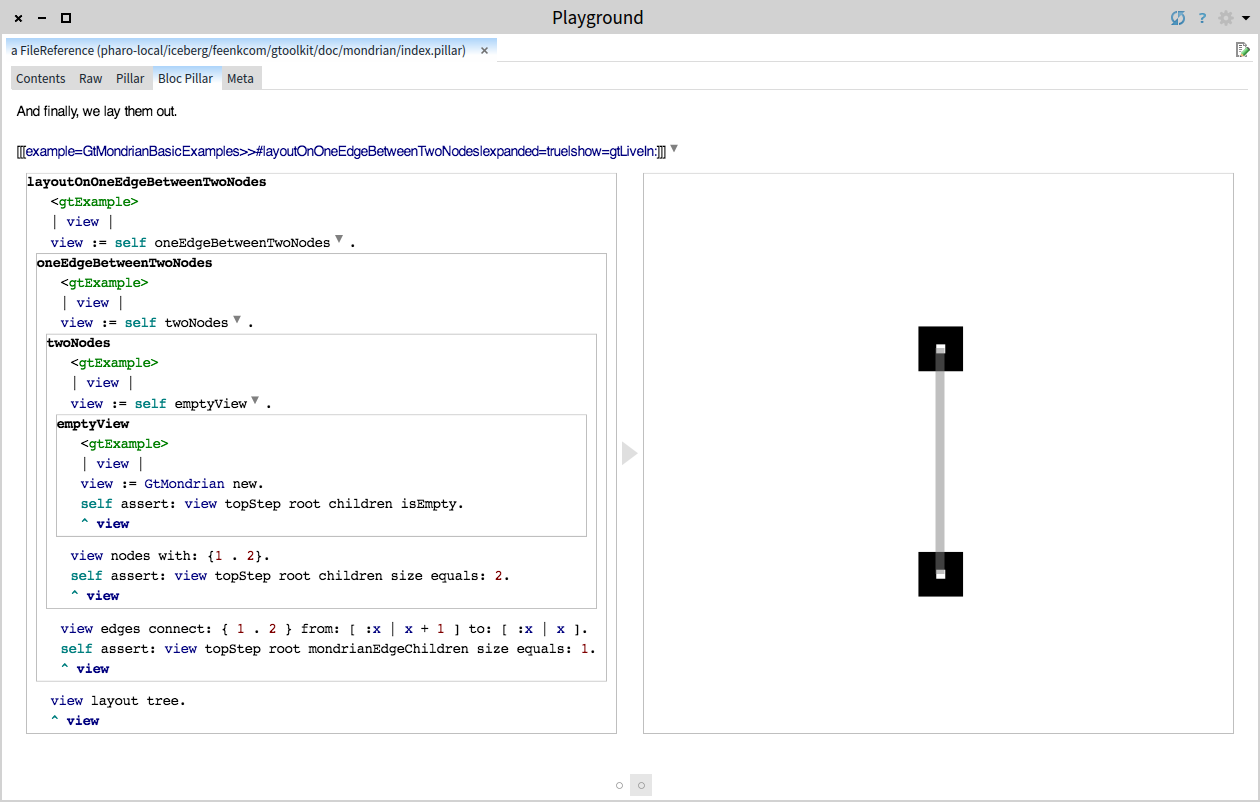
\includegraphics[width=0.95\columnwidth]{images/documenter-mondrian-expanded-examples.png}
\caption{Live preview of the example result within the Documenter}
\figlabel{GtDocumenterMondrianExpandedExamples}
\end{figure}

As shown on the \figref{GtDocumenterMondrianExpandedExamples} the Documenter facilitates an ability of the editor to mix visual components with text, in this case by recursively composing editors with each other in order to expand example's dependencies. It only becomes possible if we remove any constraints and enforce editor to treat all contained graphical components uniformly.

%===================================================================================================
%===================================================================================================
%========================================== C O N C L U S I O N  ========================================
%===================================================================================================
%===================================================================================================

\chapter {Conclusion and Future Work}

This work only scratches a surface of what can be done with a text editor. We already saw that it allows us to implement features and provide new experiences that are simply not possible in other editors. There is still a lot that should be done and we have to walk through a long path that lies in front of us. While the basic infrastructure and underlying model is in place the editor in its current state misses some important for usability features normally used during day-to-day activities such as copy-paste, keyboard shortcuts, multiple text selection and smart cursor navigation. The Moldable Editor does not yet provide an auto-completion mechanism or common decorators which include line numbers, clickable links or code critiques adornments.

Nevertheless, this work proved that it is indeed possible to implement a text editor that can be represented in a single composition tree of visual elements. More importantly, it showed that such an editor not only can exist on paper or as a prototype but can actually be performant enough to be usable. It scales well and is capable of opening large pieces of text. The choice of the underlying Rope data structure turned out to be a good idea. Its persistence property helped us to deal with text synchronisation problems in case of multithreaded use and background text styling.

One more application for this text editor is code snippets \footnote{\url{http://scg.unibe.ch/wiki/projects/Snippets-GTPlayground}} that we consider a future work. The idea would be to create an interface that allows users to split a single playground script into multiple independent \textit{snippets} that can be executed and managed independently.

%===================================================================================================
%===================================================================================================
%============================================ A N L E I T U N G  ========================================
%===================================================================================================
%===================================================================================================

\chapter {Anleitung zu wissenschaftlichen Arbeiten}

The Moldable Editor is a part of Brick\footnote{\url{https://github.com/pharo-graphics/Brick}}, a widget library on top of \textit{Bloc}, new low level vector graphical framework for \textit{Pharo}.

It can be installed in Pharo 6 or later by executing the following script in \textit{Playground}:
\begin{lstlisting}[language=Smalltalk, caption={Brick installation script},captionpos=b, label={lst:BrickInstallationScript}]
Metacello new
    baseline: 'Brick';
    repository: 'github://pharo-graphics/Brick/src';
    load: #core
\end{lstlisting}

The applications of the Moldable Editor (Transcript, Connector and Documenter) are part of the Glamorous Toolkit (GT)\footnote{\url{https://github.com/feenkcom/gtoolkit}}, which is the second generation of GT\footnote{\url{http://gtoolkit.org/}} that is based on the Bloc project.

It can be installed with the help of the following script:

\begin{lstlisting}[language=Smalltalk, caption={GToolkit installation script},captionpos=b, label={lst:GToolkitInstallationScript}]
Metacello new
   baseline: 'GToolkit';
   repository: 'github://feenkcom/gtoolkit/src';
   load.
\end{lstlisting}



%END Doc
%-------------------------------------------------------

\bibliography{thesis}
\bibliographystyle{plain}

\end{document}